\documentclass [11pt,twoside]{article}
\usepackage[utf8]{inputenc}
\usepackage[T1]{fontenc}

%Page margins, header and footer positions
\usepackage{geometry}
 \geometry{
 a4paper,
 total={210mm,297mm},
 left=25mm,
 right=25mm,
 top=30mm,
 bottom=25mm,
 headsep=7mm}

\interfootnotelinepenalty=10000

%To display filling dots in the TOC for all entries
\usepackage[titles]{tocloft}
\renewcommand{\cftsecleader}{\cftdotfill{\cftdotsep}}

%Define new header and footer style
\usepackage{fancyhdr}

\pagestyle{fancy}
\fancyhf{}
\lhead{\color{Gray}{\small{CodeKataBattle project by Russo Mario and Picone Paolo}}}
\lfoot{\textcolor{Gray}{\small{Copyright © 2023, Russo Mario and Picone Paolo – All rights reserved}}}
\rfoot{\textcolor{Gray}{\thepage}}
\renewcommand{\headrulewidth}{0pt}

%PACKAGES
\usepackage{wasysym}
\usepackage{pifont}

\newcommand{\supported}{\ding{52}\xspace}
\newcommand{\unsupported}{\ding{55}\xspace}
\newcommand{\partsupported}{\textcolor{black!40}{\ding{52}}\xspace}
\newcommand{\lowsupported}{\textcolor{black!20}{\ding{52}}\xspace}
\newcommand{\unknowsupported}{\textbf{?}\xspace}

%Font: Times
\usepackage{times}
%Change monospaced font
\renewcommand{\ttdefault}{lmtt}

%tables
\usepackage{tabu}
\usepackage{tabularx}
\usepackage{ltablex}
\usepackage{longtable}
\usepackage{float} % To allow the use of H modifier in long tables

%landscape mode
\usepackage{pdflscape}
\usepackage{rotating}
\usepackage{caption}

%make landscape mode be sensitive to even and odd pages
%start
\def\myrotate{\ifodd\c@page\else-\fi 90}
\makeatletter
\global\let\orig@begin@landscape=\landscape%
\global\let\orig@end@landscape=\endlandscape%
\gdef\@true{1}
\gdef\@false{0}
\gdef\landscape{%
    \global\let\within@landscape=\@true%
    \orig@begin@landscape%
}%
\gdef\endlandscape{%
    \orig@end@landscape%
    \global\let\within@landscape=\@false%
}%
\@ifpackageloaded{pdflscape}{%
    \gdef\pdf@landscape@rotate{\PLS@Rotate}%
}{
    \gdef\pdf@landscape@rotate#1{}%
}
\let\latex@outputpage\@outputpage
\def\@outputpage{
    \ifx\within@landscape\@true%
        \if@twoside%
            \ifodd\c@page%
                \gdef\LS@rot{\setbox\@outputbox\vbox{%
                    \pdf@landscape@rotate{-90}%
                    \hbox{\rotatebox{90}{\hbox{\rotatebox{180}{\box\@outputbox}}}}}%
                }%
            \else%
                \gdef\LS@rot{\setbox\@outputbox\vbox{%
                    \pdf@landscape@rotate{+90}%
                    \hbox{\rotatebox{90}{\hbox{\rotatebox{0}{\box\@outputbox}}}}}%
                }%
            \fi%
        \else%
            \gdef\LS@rot{\setbox\@outputbox\vbox{%
                \pdf@landscape@rotate{+90}%
                \hbox{\rotatebox{90}{\hbox{\rotatebox{0}{\box\@outputbox}}}}}%
            }%
        \fi%
    \fi%
    \latex@outputpage%
}
\makeatother
%end

%graphics
\usepackage{graphicx}
\usepackage[dvipsnames, table]{xcolor}
%If you upload images from PC, you need to insert code for the path here (different for Windows and Unix OS)

%References
%\usepackage{xpatch}
%\usepackage[backend=biber, style=numeric, citestyle=numeric, sorting=none]{biblatex}
%\addbibresource{main.bib}

%Other
\usepackage{ifthen}
\usepackage{xspace}
\usepackage{enumitem}
\usepackage{amssymb}
\usepackage[pdftex, colorlinks]{hyperref}
\newcommand{\comment}[1]{{\color{Red}$\blacktriangleright$ Comment: #1 $\blacktriangleleft$}}


% Some utilities\ldots
\usepackage{soul}
\usepackage{tikz}

\usetikzlibrary{calc}
\usetikzlibrary{decorations.pathmorphing}


\makeatletter

\newcommand{\defhighlighter}[3][]{%
  \tikzset{every highlighter/.style={color=#2, fill opacity=#3, #1}}%
}

\defhighlighter{yellow}{.5}

\newcommand{\highlight@DoHighlight}{
  \fill [ decoration = {random steps, amplitude=1pt, segment length=15pt}
        , outer sep = -15pt, inner sep = 0pt, decorate
       , every highlighter, this highlighter ]
        ($(begin highlight)+(0,8pt)$) rectangle ($(end highlight)+(0,-3pt)$) ;
}

\newcommand{\highlight@BeginHighlight}{
  \coordinate (begin highlight) at (0,0) ;
}

\newcommand{\highlight@EndHighlight}{
  \coordinate (end highlight) at (0,0) ;
}

\newdimen\highlight@previous
\newdimen\highlight@current

\DeclareRobustCommand*\highlight[1][]{%
  \tikzset{this highlighter/.style={#1}}%
  \SOUL@setup
  %
  \def\SOUL@preamble{%
    \begin{tikzpicture}[overlay, remember picture]
      \highlight@BeginHighlight
      \highlight@EndHighlight
    \end{tikzpicture}%
  }%
  %
  \def\SOUL@postamble{%
    \begin{tikzpicture}[overlay, remember picture]
      \highlight@EndHighlight
      \highlight@DoHighlight
    \end{tikzpicture}%
  }%
  %
  \def\SOUL@everyhyphen{%
    \discretionary{%
      \SOUL@setkern\SOUL@hyphkern
      \SOUL@sethyphenchar
      \tikz[overlay, remember picture] \highlight@EndHighlight ;%
    }{%
    }{%
      \SOUL@setkern\SOUL@charkern
    }%
  }%
  %
  \def\SOUL@everyexhyphen##1{%
    \SOUL@setkern\SOUL@hyphkern
    \hbox{##1}%
    \discretionary{%
      \tikz[overlay, remember picture] \highlight@EndHighlight ;%
    }{%
    }{%
      \SOUL@setkern\SOUL@charkern
    }%
  }%
  %
  \def\SOUL@everysyllable{%
    \begin{tikzpicture}[overlay, remember picture]
      \path let \p0 = (begin highlight), \p1 = (0,0) in \pgfextra
        \global\highlight@previous=\y0
        \global\highlight@current =\y1
      \endpgfextra (0,0) ;
      \ifdim\highlight@current < \highlight@previous
        \highlight@DoHighlight
        \highlight@BeginHighlight
      \fi
    \end{tikzpicture}%
    \the\SOUL@syllable
    \tikz[overlay, remember picture] \highlight@EndHighlight ;%
  }%
  \SOUL@
}

\makeatother

% Common abbrev. are set as commands to ensure proper spacing after the dot
\RequirePackage{xspace}
\newcommand{\ie}{i.e.\@\xspace}
\newcommand{\aka}{a.k.a.\@\xspace}
\newcommand{\Ie}{I.e.\@\xspace}
\newcommand{\cf}{cf.\@\xspace}
\newcommand{\Cf}{Cf.\@\xspace}
\newcommand{\eg}{e.g.\@\xspace}
\newcommand{\Eg}{E.g.\@\xspace}
\newcommand{\etal}{et al.\@\xspace}
\newcommand{\etc}{etc.\@\xspace}
\newcommand{\wrt}{w.r.t.\@\xspace}
\newcommand{\Wrt}{W.r.t.\@\xspace}



\date{}


\begin{document}

%TITLE PAGE

\begin{titlepage}


%LOGO

{\begin{table}[t!]
\centering
\begin{tabu} to \textwidth { X[1.3,r,p] X[1.7,l,p] }
\textcolor{Blue}
{\textbf{\small{CodeKataBattle project by Russo Mario and Picone Paolo}}} & 
\includegraphics[scale=0.5]{Images/PolimiLogo}
\end{tabu}
\end{table}}~\\ [7cm]

%TITLE 

\begin{flushleft}

%Replace the text string with your title
{\textcolor{Blue}{\textbf{\Huge{Requirement Analysis and Specification
        Document}}}} \\ [1cm]

\end{flushleft}

\end{titlepage}

%Define deliverable specific info
%Replace cell contents where needed
\begin{table}[h!]
\begin{tabu} to \textwidth { X[0.3,r,p] X[0.7,l,p] }
\hline

\textbf{Deliverable:} & RASD\\
\textbf{Title:} & Requirement Analysis and Verification Document \\
\textbf{Authors:} & Picone Paolo and Russo Mario\\
\textbf{Version:} & 1.0 \\ 
\textbf{Date:} & 20-November-2023 \\
\textbf{Download page:} & https://github.com/piconepaolo/PiconeRusso \\
\textbf{Copyright:} & Copyright © 2023, Picone Paolo and Russo Mario – All rights reserved \\
\hline
\end{tabu}
\end{table}




\setcounter{page}{2}


%------------------------------------------------------------------------------------------------------------------------------------------------
\newpage
\addcontentsline{toc}{section}{Table of Contents}
\tableofcontents
\newpage
\addcontentsline{toc}{section}{List of Figures}
\listoffigures
\addcontentsline{toc}{section}{List of Tables}
\listoftables

%------------------------------------------------------------------------------------------------------------------------------------------------
\clearpage
{\color{Blue}{\section{Introduction}}}
\label{sect:introduction}
\subsection{Purpose}
The motivation behind the existence of the CodeKataBattle platform is to provide students with a dedicated platform for practicing their programming skills. The platform aims to create a competitive environment where teams of students can participate in programming tournaments and solve programming challenges.

By offering a platform specifically designed for programming practice, CodeKataBattle aims to provide students with a structured and engaging way to improve their coding abilities. The competitive nature of the platform adds an extra layer of motivation and excitement, encouraging students to push their limits and strive for excellence.

Overall, the motivations behind the existence of the CodeKataBattle platform are to create a dedicated space for programming practice, foster healthy competition among students, and provide a means for tracking and improving programming skills.

\subsubsection{Goals}
[G1] Educator can create a tournament
[G2] Educator can create battles for the tournament
[G3] Student can compete in a tournament
[G4] Team of students can compete in a battle
[G5] Student is evaluated based on the performance in the battle
[G6] Student are notified about upcoming tournaments

\subsection{Scope}
The scope of this project is to develop a platform (CodeKataBattle) that is intended to be used by students for practicing their programming skills.
The platform is used in a competitive setting where teams of students compete against each other in tournaments where they are given programming problems to solve.
The platform is equipped with a ranking system that ranks that assigns...
Additionally, the platform incorporates a ranking system that assigns scores to participants based on their performance in the tournaments. This ranking system not only adds a competitive element but also allows students to track their progress and compare their skills with others. This can be a valuable tool for self-assessment and identifying areas for improvement.

% Github Actions

%------------------------------------------------------------------------------------------------------------------------------------------------
\clearpage
{\color{Blue}{\section{Overall Description}}}
\label{sect:overview}
\subsection{Product Perspective}
\subsubsection{Scenarios}
\begin{enumerate}
    \item \textbf{Educator creates a battle for a tournament} \\
    The educator who wants to create a battle in a tournament for which he is the creator, or for which he has the permission to create battles.
    The creation of a battle consists of in:
    \begin{itemize}
        \item Set the deadline for registration of teams
        \item Set the deadline for the submission of solutions
        \item Set the minimum and maximum number of students per team
        \item Upload the code kata to the CKB platform
    \end{itemize}
    Once the battle is created, the students registered at that tournament are notified by CKB about the upcoming battle. The CKB platform will also create a new repository on Github for the battle, and will invite the students to fork it.
    \item \textbf{Student invite other students to join the team} \\
    Roberto is a student who wants to participate in a battle. He has already registered in the tournament in which the battle has been created, and he has been notified about the upcoming battle. He wants to invite other students to join his team for the battle. He can do this by sending an invitation to the other students, who will receive a notification about the invitation. The other students can accept or decline the invitation. If they accept, they will be added to the team and they will be able to compete as a team in a battle.
    Even if the students invited have accepted the invitation the partecipation to the battle is not guaranteed since the educator could have set a maximum number of students per team.
    \item \textbf{Student push the solution of the battle to the forked repository} \\
    The team A have been working on the solution for the battle for a while and it seems to be passing all the tests provided in the code kata. Since the time being is before the submission deadline the team push the solution to the forked repository. This will trigger the CKB platform to evaluate the solution and update the score of the team in the battle. In the case that the submission date is after the submission deadline the push will not trigger another evaluation of the solution by the CKB platform.
    \item \textbf{Educator manually updates the score of a team} \\
    Giacomo is an educator who has created a battle for a tournament in which he has been invited by another collegue. Once the submission deadline is expired he wants to manually assess the score of a team to cover all the aspects that the CKB platform cannot evaluate. To do this he access through the CKB platform the battle page and he can see the list of teams that have submitted a solution. He can then manually update the score of a team by clicking on the `Update score' button. This will open a form where he can modify the current score of the team previously evaluated by the platform. Once he is satisfied with the score he can click on the `Save' button to save the new score for the team. The new score will be visible to the team and to the other students subscribed to the tournament.
    \item \textbf{CKB notifies students about the result of the tournament} \\
    When an Educator closes a tournament, the CKB platform will notify all the students subscribed to the tournament about the result of the tournament. The notification will contain the list of the teams that have participated in the tournament and their final score.

\end{enumerate}
\subsubsection{Domain class Diagram}
In \figurename~\ref{fig:domain_class_diagram} is shown the domain class diagram of the CKB platform. This diagram shows the main entities of the system and their relationships.
\begin{itemize}
    \item \textbf{User}: is the main entity of the system. It represents a user of the CKB platform. It can be either a student or an educator.
    \item \textbf{Student}: is a user of the CKB platform. It can participate in tournaments and battles. It can also create teams and invite other students to join them.
    \item \textbf{Educator}: is a user of the CKB platform. It can create and manage tournaments and battles. He can also invite other educators to join a tournament. He also uploads the code kata to the CKB platform for a battle.
    \item \textbf{Tournament}: is a competition between teams of students. It is created by an educator and it can be joined by students. It can contain multiple battles.
    \item \textbf{Battle}: is a competition between teams of students. It is created by an educator and it can be joined by students. It is part of a tournament and it can contain multiple teams.
    \item \textbf{Team}: is a group of students that compete together in a battle. It is created by a student and it can be joined by other students.
    \item \textbf{Invitation}: is a request sent by a student to another student to join a team. It can be accepted or declined by the receiver.
    \item \textbf{Code Kata}: is the description of the problem that the student have to solve in a battle. It contains the description of the software project to be implemented, the test cases that the solution must pass and the build automation scripts.
    \item \textbf{Score}: is the score of a team in a battle. It is calculated by the CKB platform based on the evaluation of the submission of the team. It also adds up the manual score given by the educator. The score assigned to the team, for each battle, is also the score of the students in the tournament.
    \item \textbf{Ranking}: is the ranking of the students in a tournament. It is calculated by the CKB platform based on the score of the students in the battles of the tournament in which they have participated.
    \item \textbf{Repository}: is the repository on Github that contains the code kata and the build automation scripts for a battle. It is created by the CKB platform when a battle is created. It is forked by the teams that want to compete in the battle.
    \item \textbf{Forked Repository}: is the repository forked by a team of students to compete in a battle. It contains the code kata and the build automation scripts for the battle. Each push to the forked repository will trigger the CKB platform to evaluate the submission of the team and update the score of the team.
    \item \textbf{Submission}: is the code that a team of students have implemented for a battle or a subsequent version of a previous submission. It is pushed to the forked repository of the battle by a team member. The CKB platform will evaluate the submission and update the score of the team.
    \item \textbf{Evalutation}: is the evaluation of a submission. It is done by the CKB platform based on the code kata provided by the educator. It is done automatically by the CKB platform when a submission is pushed to the forked repository of the battle. It is also done manually by the educator when he updates the score of a team.
\end{itemize}

\begin{figure}[H]
    \centering
    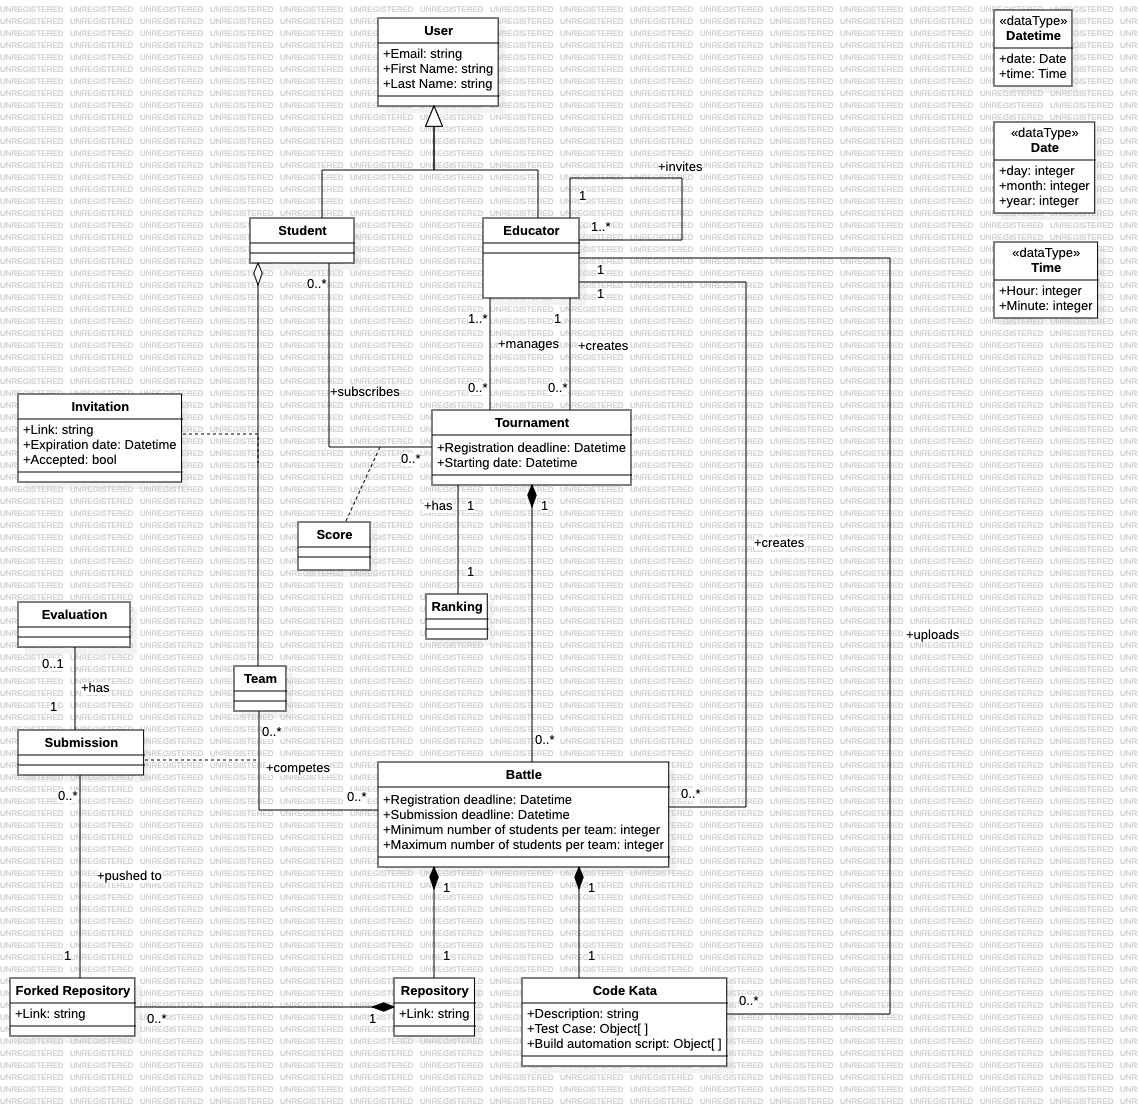
\includegraphics[width=1\textwidth]{Diagrams/DomainClassDiagram.jpg}
    \caption{Domain class diagram}
    \label{fig:domain_class_diagram}
\end{figure}

\subsubsection{Statecharts}

\textbf{Statechart of a Tournament} \\
The statechart in \figurename~\ref{fig:statechart_tournament} shows the possible states of a tournament. A tounament can be in two principal states: ``In Progress'' or ``Closed''. A tournament is in the ``In Progress'' state when it is created by an educator. When the educator closes the tournament, it will be in the ``Closed'' state.
\begin{figure}[H]
    \centering
    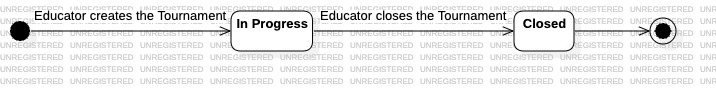
\includegraphics[width=1\textwidth]{Diagrams/TournamentStateChart.jpg}
    \caption{Statechart of a Tournament}
    \label{fig:statechart_tournament}
\end{figure}
\textbf{Statechart of a Battle} \\
The statechart in \figurename~\ref{fig:statechart_battle} shows the possible states of a battle. When the educator creates a battle it will be in initial ``Created'' state. When the date of the registration deadline is expired, the batlle will be in ``Registration closed'' state. When registration is closed, the platform sends the link of the repository to the students that have registered to the tournament. After the link is sent the battle will be in ``Accepting submissions'' state. When the date of the submission deadline is expired, the battle will be in ``Consolidation'' state. In this state the educator can manually update the score of a team. When the educator closes  the tournament and finalizes the evaluations, it will be in the ``Closed'' state.
\begin{figure}[H]
    \centering
    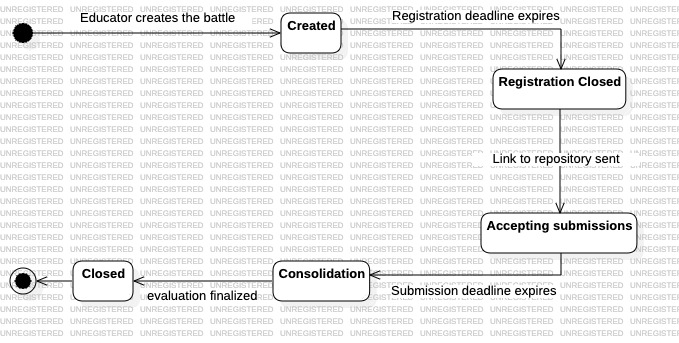
\includegraphics[width=1\textwidth]{Diagrams/BattleStateChart.jpg}
    \caption{Statechart of a Battle}
    \label{fig:statechart_battle}
\end{figure}

\subsection{Product Functions}
\subsubsection{User registration and login}
The CKB platform allows the users to register and login to the platform. The registration is required to access the platform and to use its functionalities. The registration process requires the user to provide a valid email address and a password. The email address will be used to identify the user in the platform \ie{User or Educator}. The password will be used to authenticate the user when he wants to login to the platform. The CKB platform will send a confirmation email to the user to verify the email address. The user will be able to login to the platform only after the email address has been verified.
\subsubsection{Creation of a tournament}
The CKB platform allows the educators to create tournaments. The Educator will be prompted to provide the name of the tournament and the deadline for the registration. When the tournament is created, the CKB platform will send a notification to all the students registered to the platform. The Educator, that has done the creation, will be able to invite other educators to join the tournament.
\subsubsection{Creation of a battle}
The CKB platform allows the educators to create battles. The Educator will be prompted to provide the name of the battle, the deadline for the registration, the deadline for the submission of the solutions, the minimum and maximum number of students per team and the code kata. When the battle is created, the CKB platform will send a notification to all the students subscribed to the tournament. The CKB platform will also create a new repository on Github for the battle, and will invite the students to fork it.
\subsubsection{Creation and joining of a team}
The students in order to compete in a battle must form or join a team. The CKB platform allows the students to create teams by inviting other students to join their team. The student will be prompted to provide the name of the team, as well as the list of the emails of the students that he wants to invite. The CKB platform will send a notification to the invited students. The invited students will be able to accept or decline the invitation. If they accept, they will be added to the team as long as the minimum and maximum number of students per team (set by the educator) is respected.
\subsubsection{Submission and evaluation of a solution}
The students of a team that are competing for a battle can submit their solution to the CKB platform in order to be evaluated. The submission consists of pushing the code that the team has implemented for the battle to the forked repository of the battle previously created by the CKB platform and forked by the team.
The CKB platform will evaluate the submission using the code kata provided by the educator and will update the score of the team.
\subsubsection{Manual update of the score}
The CKB platform allows the educators to manually update the score of a team. After accessing the battle page on the CKB platform, educators can manually adjust a team's score as long as the battle is in the \textit{Consolidation stage}. This feature proves beneficial when evaluating aspects beyond the scope of automatic assessment already done by the platform. On the battle page, educators can view the list of teams that have submitted solutions. By clicking the Update Score' button, a form is opened, allowing the educator to modify the team's current score as assessed by the platform. Once satisfied with the adjustments, clicking the Save' button finalizes the new score.
\subsubsection{Notification of the result of a tournament}
Once an educator closes a tournament, the CKB platform will notify all the students subscribed to the tournament about the result of the tournament. The notification will contain the list of the teams that have participated in the tournament and their final score.
\subsubsection{Creation of the repository to sumbit the solution}
The CKB platform will create a new repository on Github for the battle, and will invite the students to fork it by sending the link of the repository to the students. The repository will contain the code kata provided by the educator and the build automation scripts. The students will be able to push their solution once they have forked the repository and set up the actions to trigger the evaluation of the solution by the CKB platform.

\subsection{User Characteristics}
The CKB platform is designed to be used by two types of users: \textit{Educators} and \textit{Students}.

\subsubsection{Educator}
The Educator is the user that manages tournaments and battles. He is able to invite other educators to join a tournament in order to grant them the permission to create battles for that tournament.
The educator is the user that creates and closes the tournaments and battles (for which he has the permissions to do so in the case he was invited).
He can set restrictions for the battles such as the deadline for the registration of teams, the deadline for the submission of solutions, the minimum and maximum number of students per team. He provides the code kata for the battle. He can also manually update the score of a team. The educator can be looked at as the administrator for a tournament and battles for that tournament. Nevertheless he cannot compete like a student in a tournament or battle.

\subsubsection{Student}
The Student is the user that participates in tournaments and battles. He can team up with other students to compete in a battle by forming teams. He can submit the solution of a battle with his team. He can also compete in multiple battles and multiple tournaments with multiple teams at the same time. The student can be looked at as the competitor in a tournament since the ranking of the tournament is per student. Nevertheless he cannot manage tournaments and battles like an educator.

\subsection{Assumptions, Dependencies and Constraints}

\subsubsection{Regulatory policies}
The CKB platform will store the informations provided by the user, such as the name, surname and email address and informations on forked repositories. This information will not be used for commercial purposes and they will not be shared with third parties.

\subsubsection{Domain assumptions}
This paragraph contains the assumptions that the CKB platform makes about the domain in which it operates. These assumptions are out of the scope of the CKB platform and they are not verified by the platform.

\begin{enumerate}[label=D\arabic*:]
    \item User must have an internet connection
    \item The Student must have a Github account
    \item The Educator must have a Github account
    \item Educator needs to be verified by the CKB platform
    \item Teams must setup the Github actions to trigger the evaluation of the solution by the CKB platform
    \item Student needs to accept the invitation to join a team
    \item Student must be registered to CKB to receive notifications about tournaments
    \item Student must be registered to the tournament to receive notifications about upcoming battles
    \item Educator can evaluate the performance of a student in a battle only if the battle is in the \textit{Consolidation} state
\end{enumerate}

%------------------------------------------------------------------------------------------------------------------------------------------------
\clearpage
{\color{Blue}{\section{Specific Requirements}}}
\label{sect:requirements}
\subsection{External Interfaces}
\subsubsection{User Interfaces}

\begin{figure}[H]
    \centering
    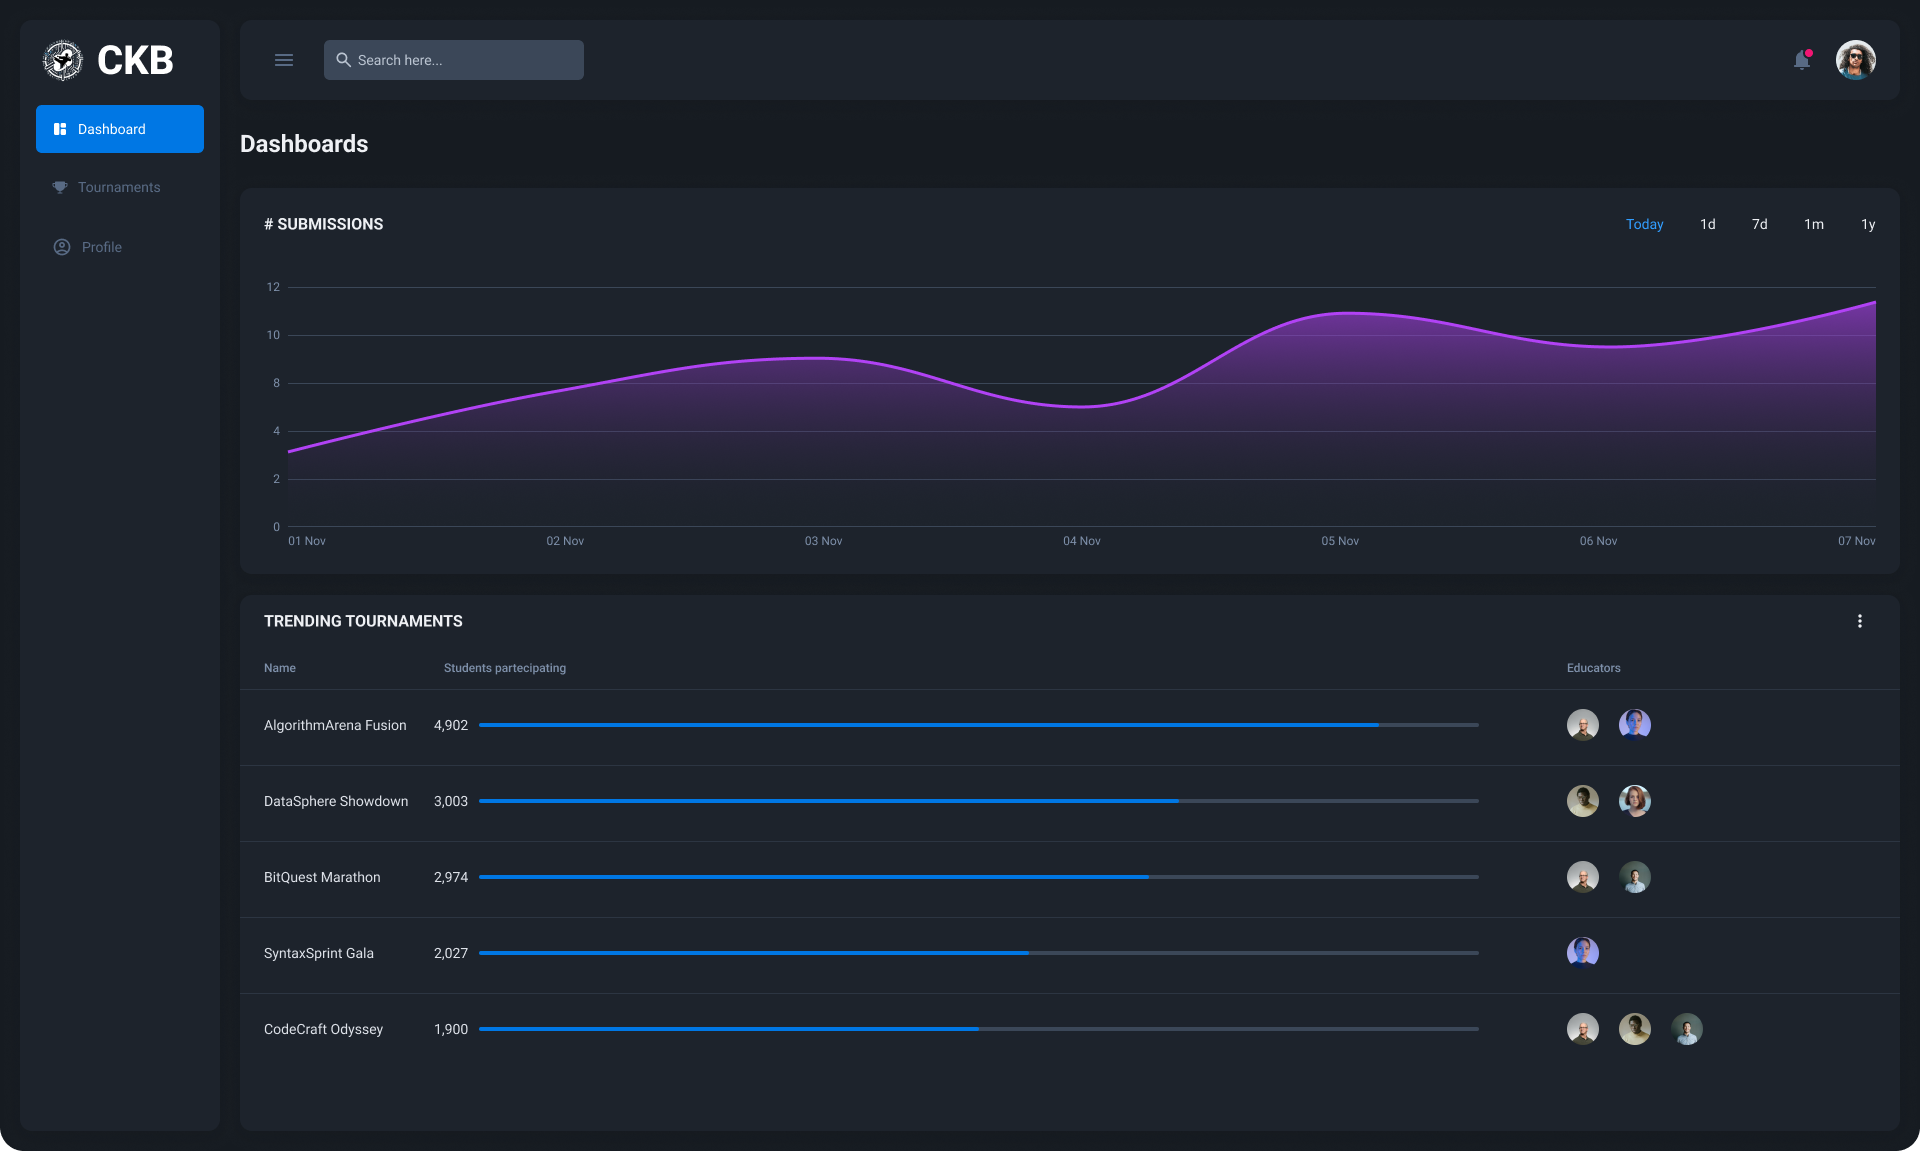
\includegraphics[width=\textwidth]{Images/Dashboard-Student.png}
    \caption{Student Dashboard}
    \label{fig:student-dashboard}
\end{figure}

\begin{figure}[H]
    \centering
    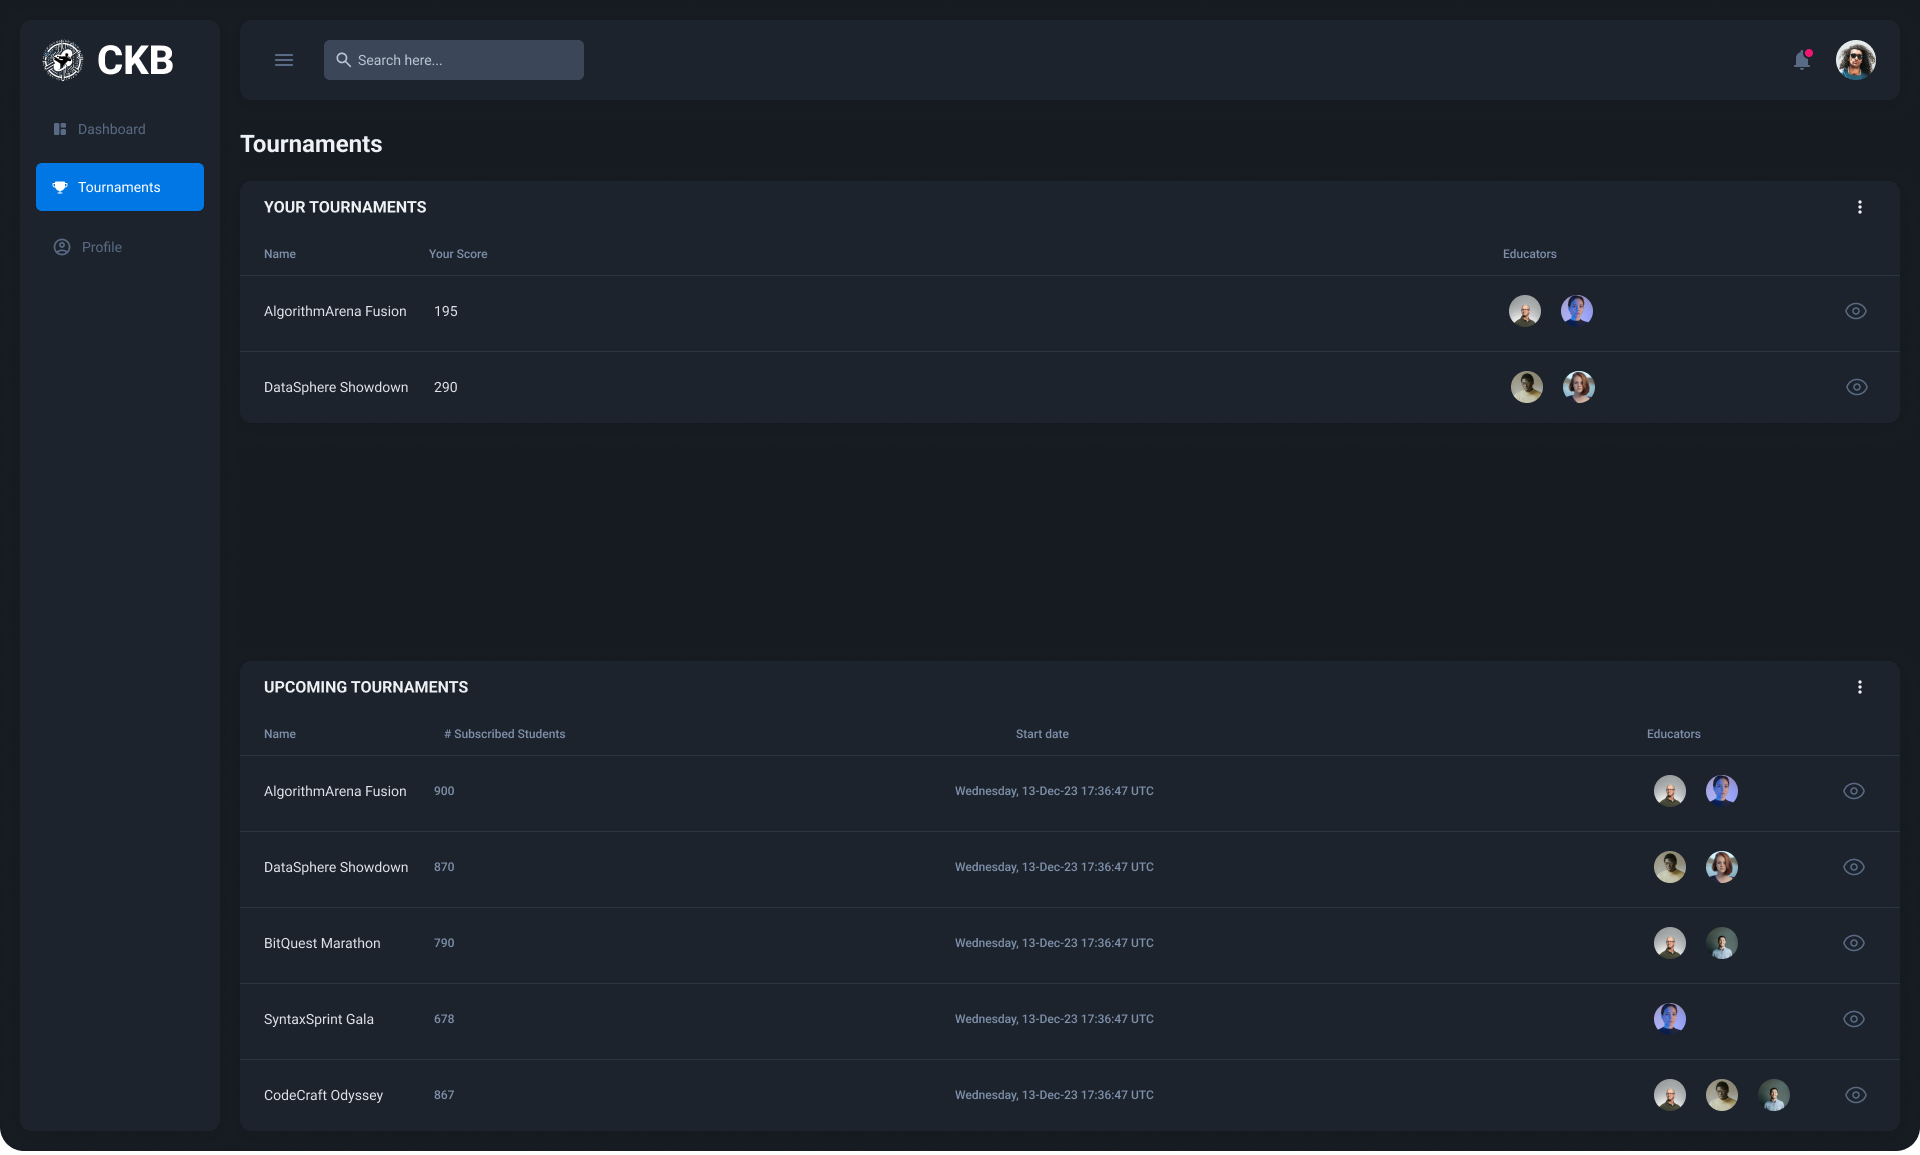
\includegraphics[width=\textwidth]{Images/Dashboard-Tournament.png}
    \caption{Student Dashboard Tournaments Tab}
    \label{fig:student-dashboard-tournaments}
\end{figure}

\begin{figure}[H]
    \centering
    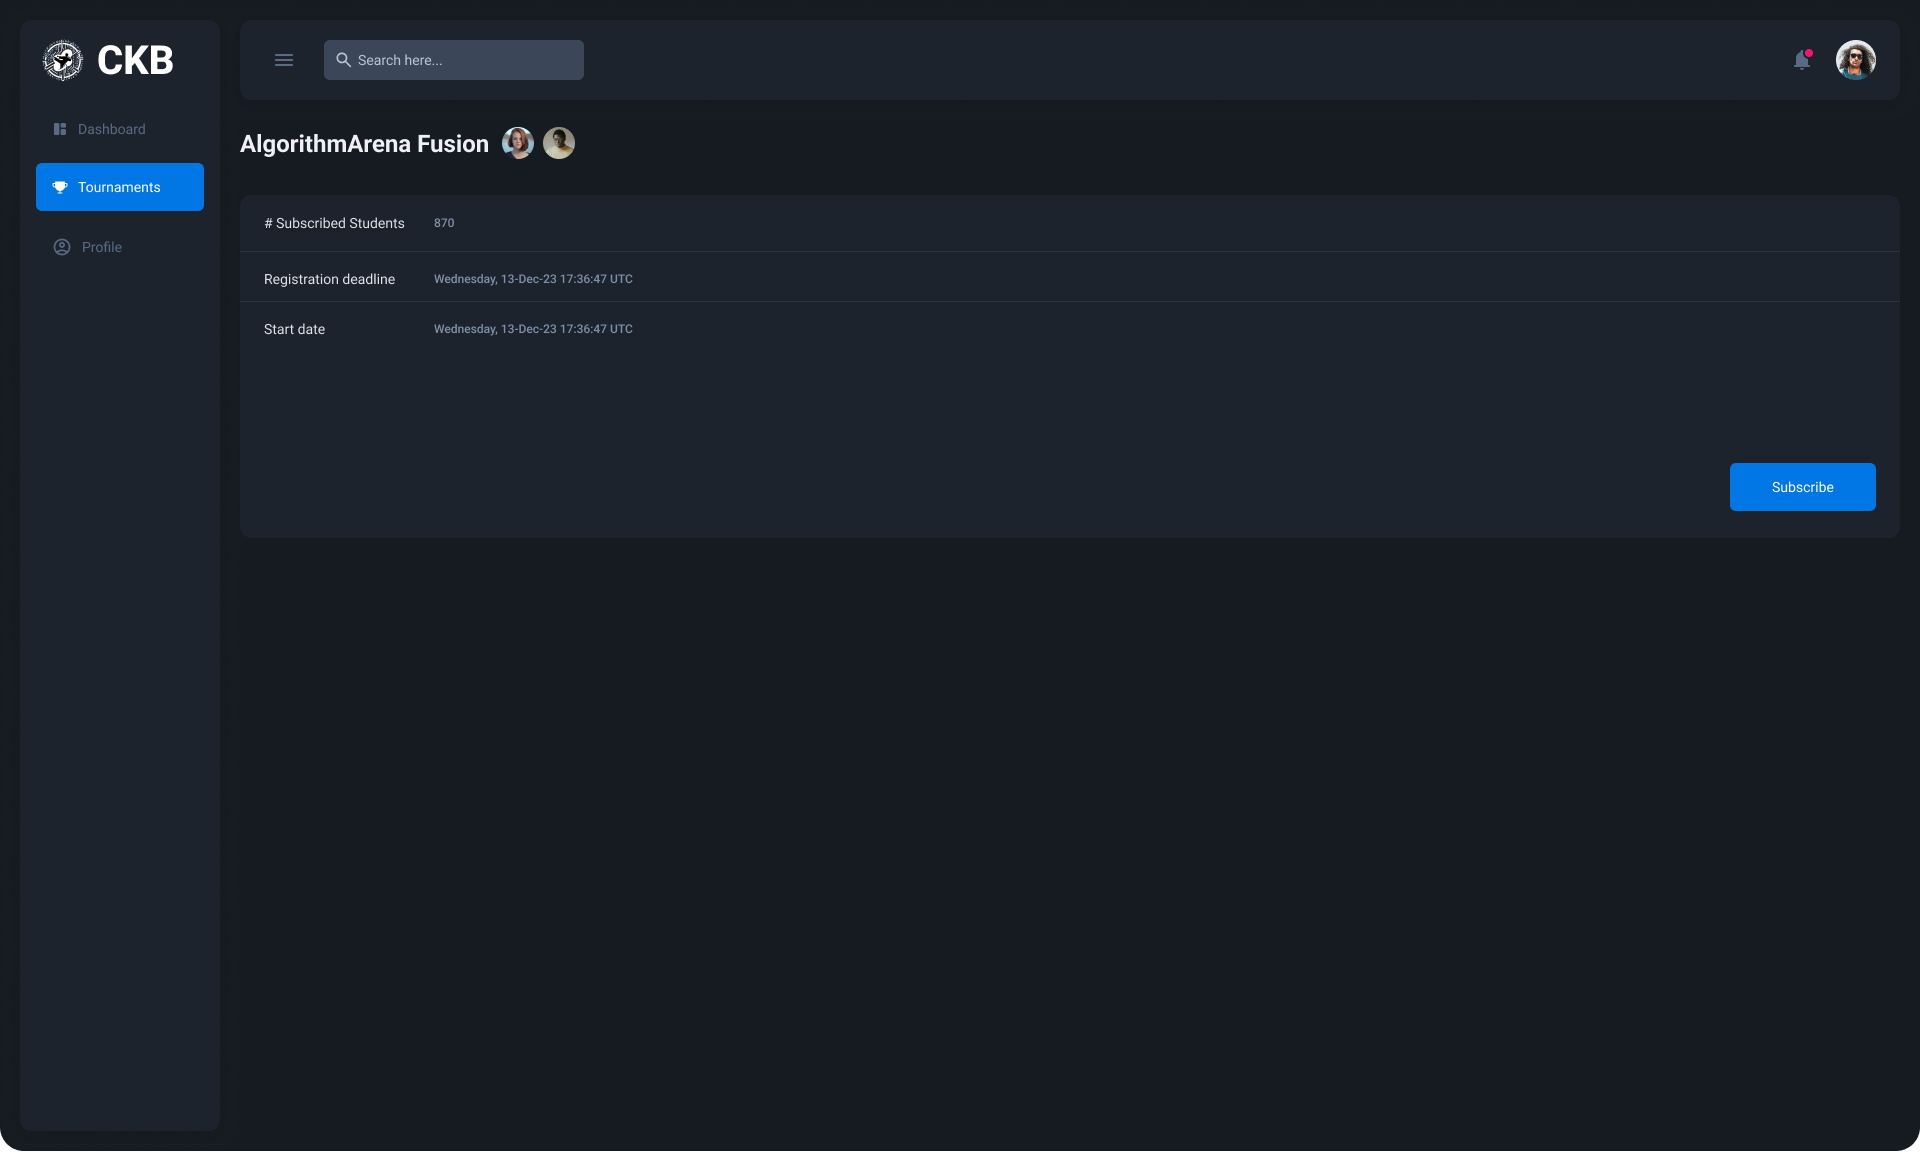
\includegraphics[width=\textwidth]{Images/Dashboard-Tournament-OverView.png}
    \caption{Student Dashboard Tournament OverView}
    \label{fig:student-Tournament-OverView}
\end{figure}

\begin{figure}[H]
    \centering
    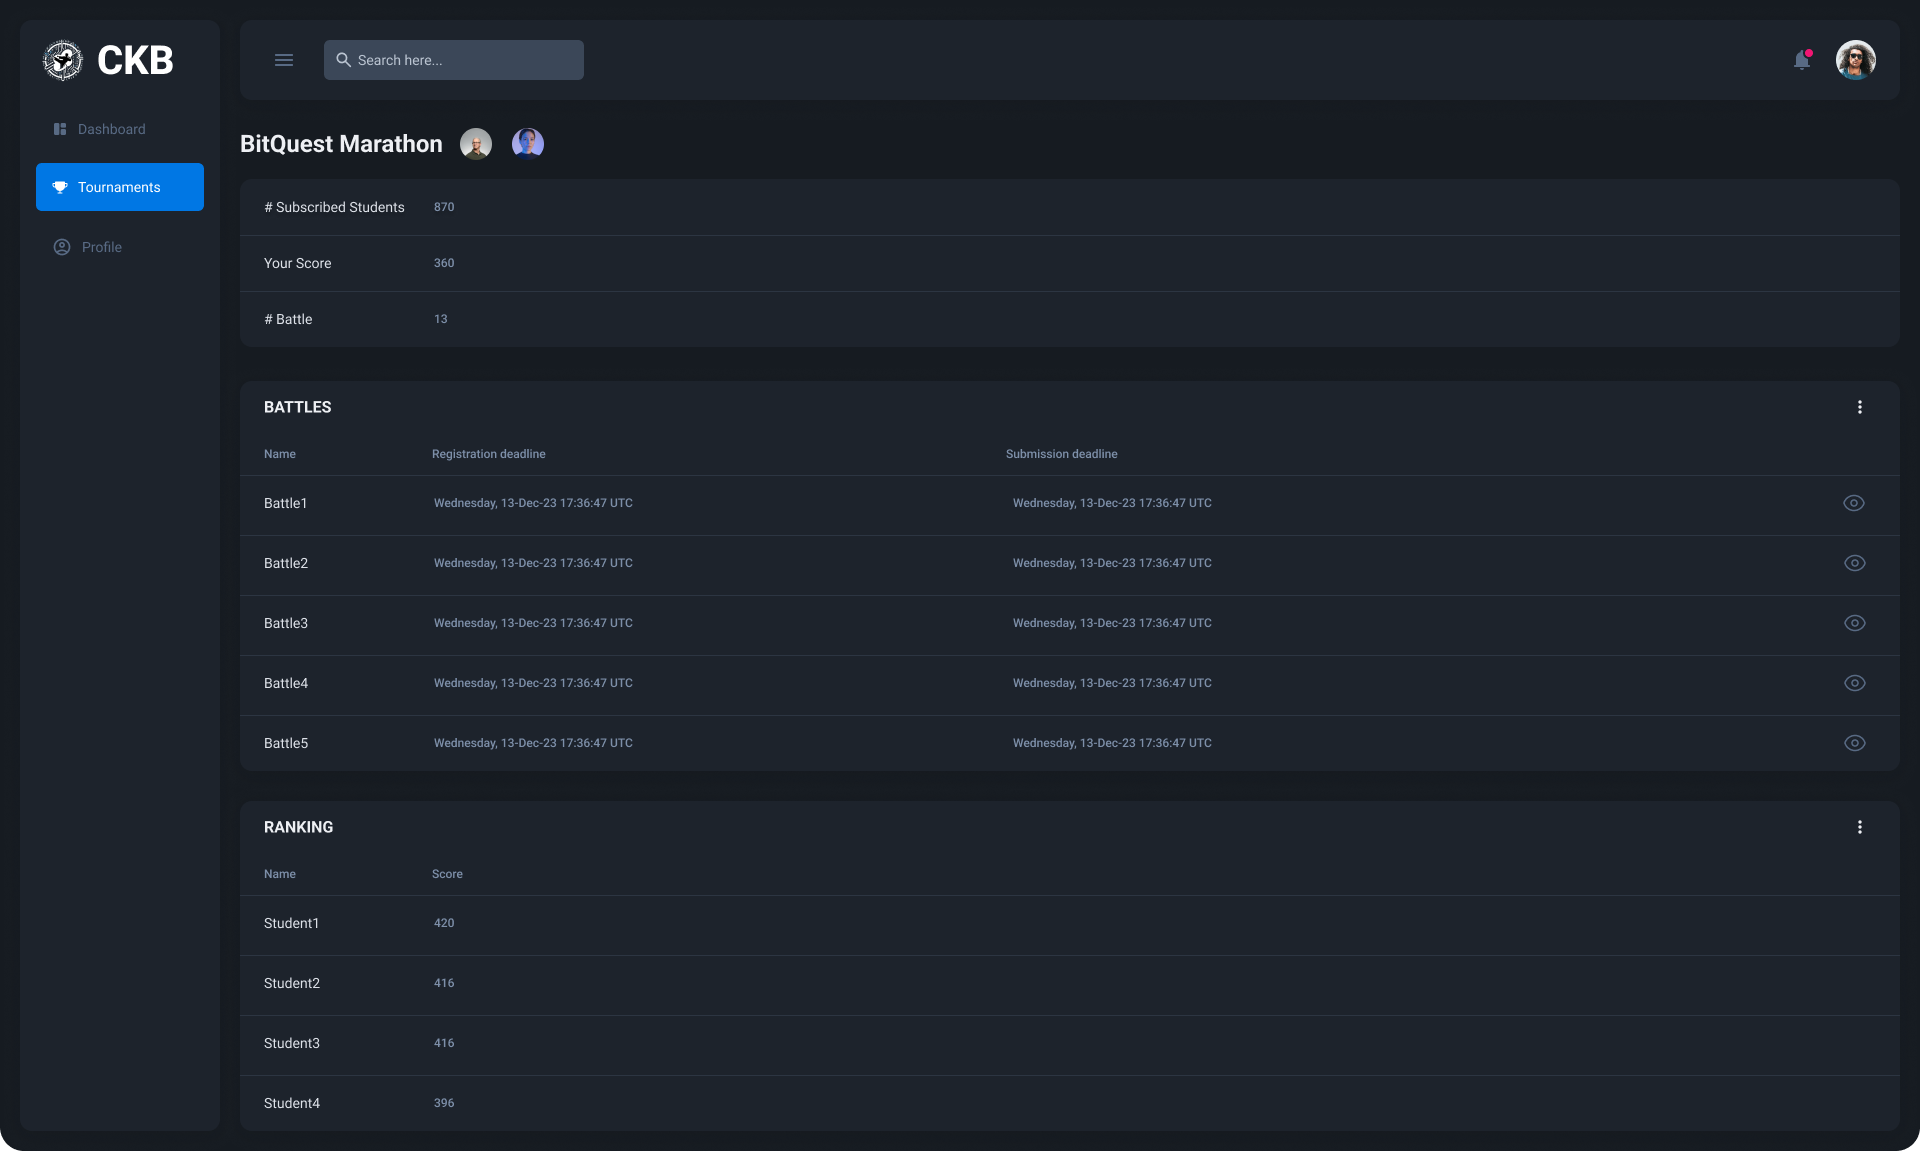
\includegraphics[width=\textwidth]{Images/Dashboard-Tournament-Ongoing.png}
    \caption{Student Dashboard Tournament Ongoing}
    \label{fig:student-Tournament-Ongoing}
\end{figure}

\begin{figure}[H]
    \centering
    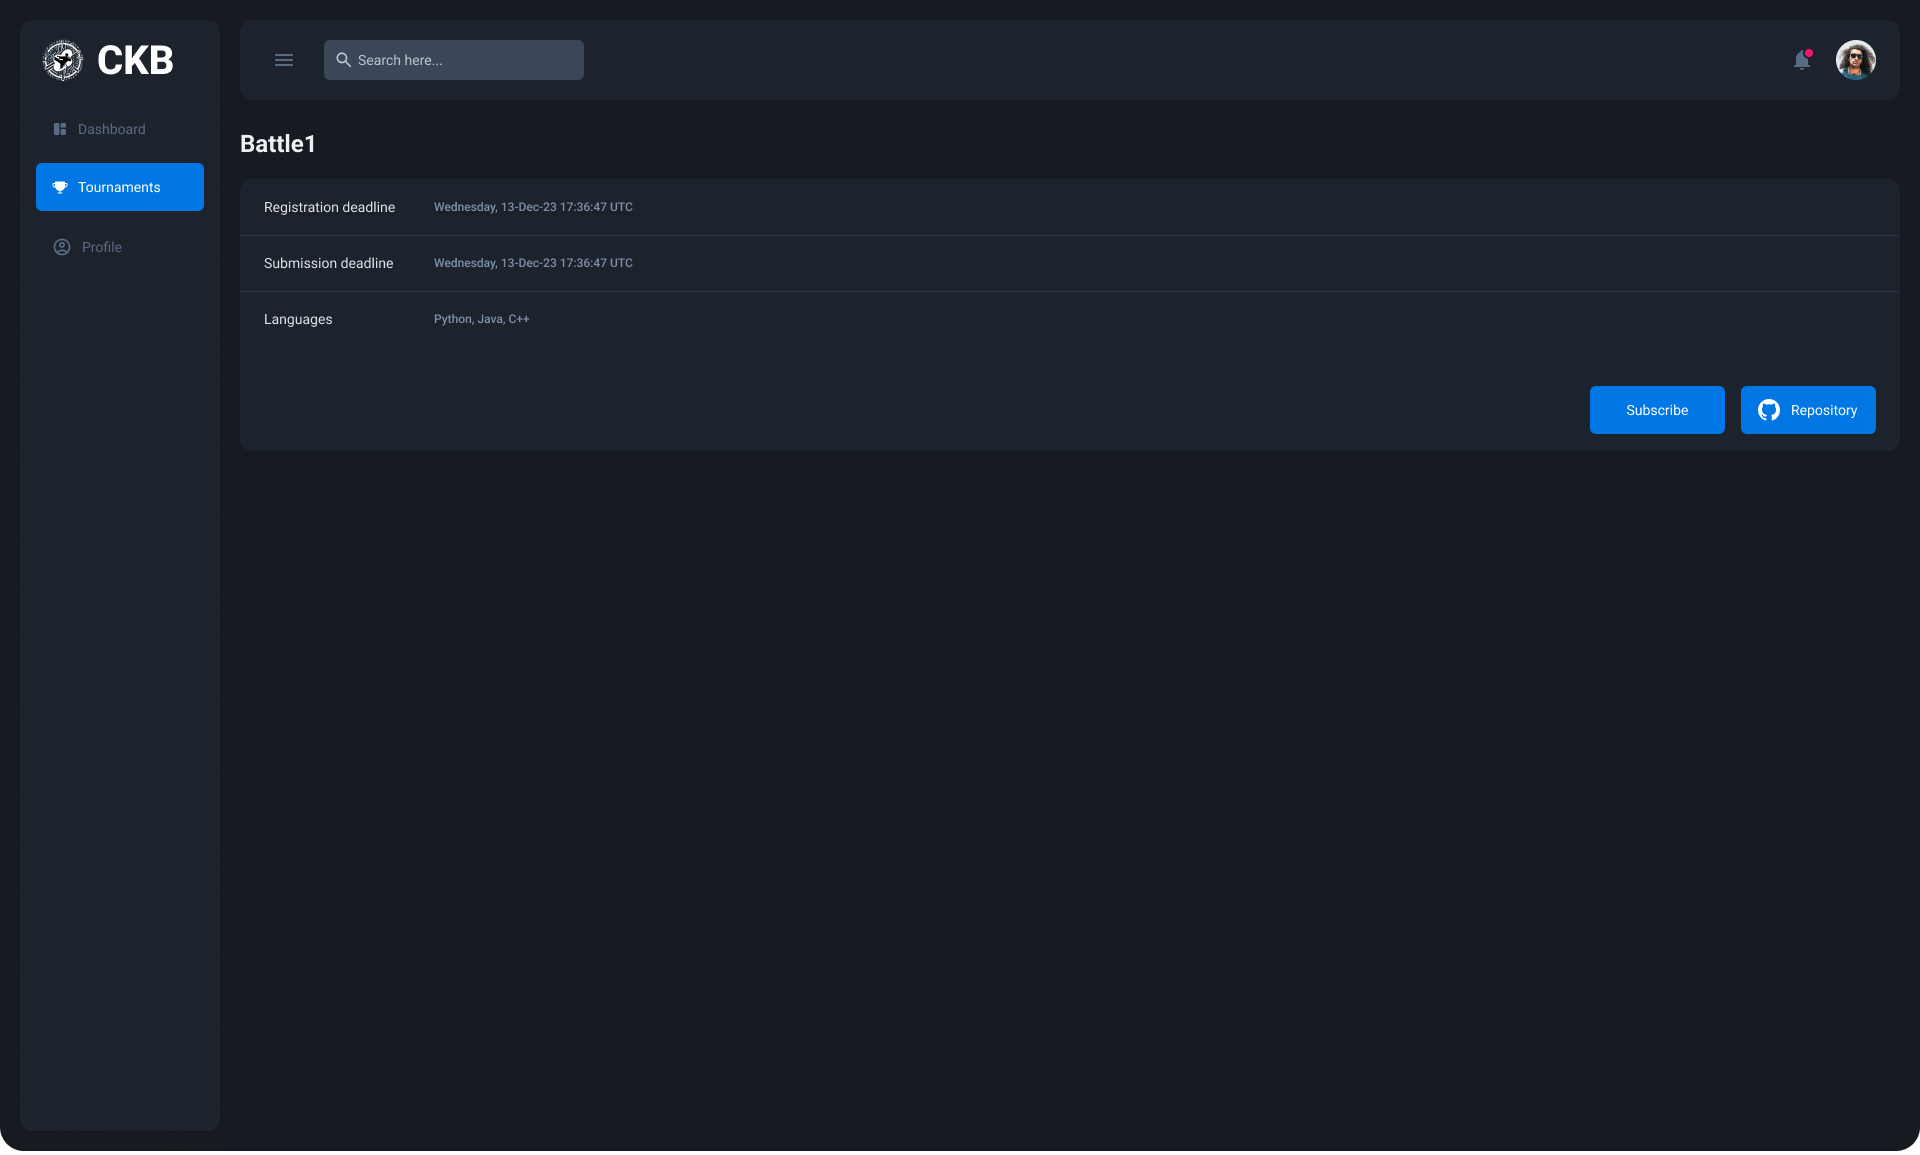
\includegraphics[width=\textwidth]{Images/Dashboard-Battle-Overview.png}
    \caption{Student Dashboard Battle Overview}
    \label{fig:student-Tournament-Completed}
\end{figure}

\begin{figure}[H]
    \centering
    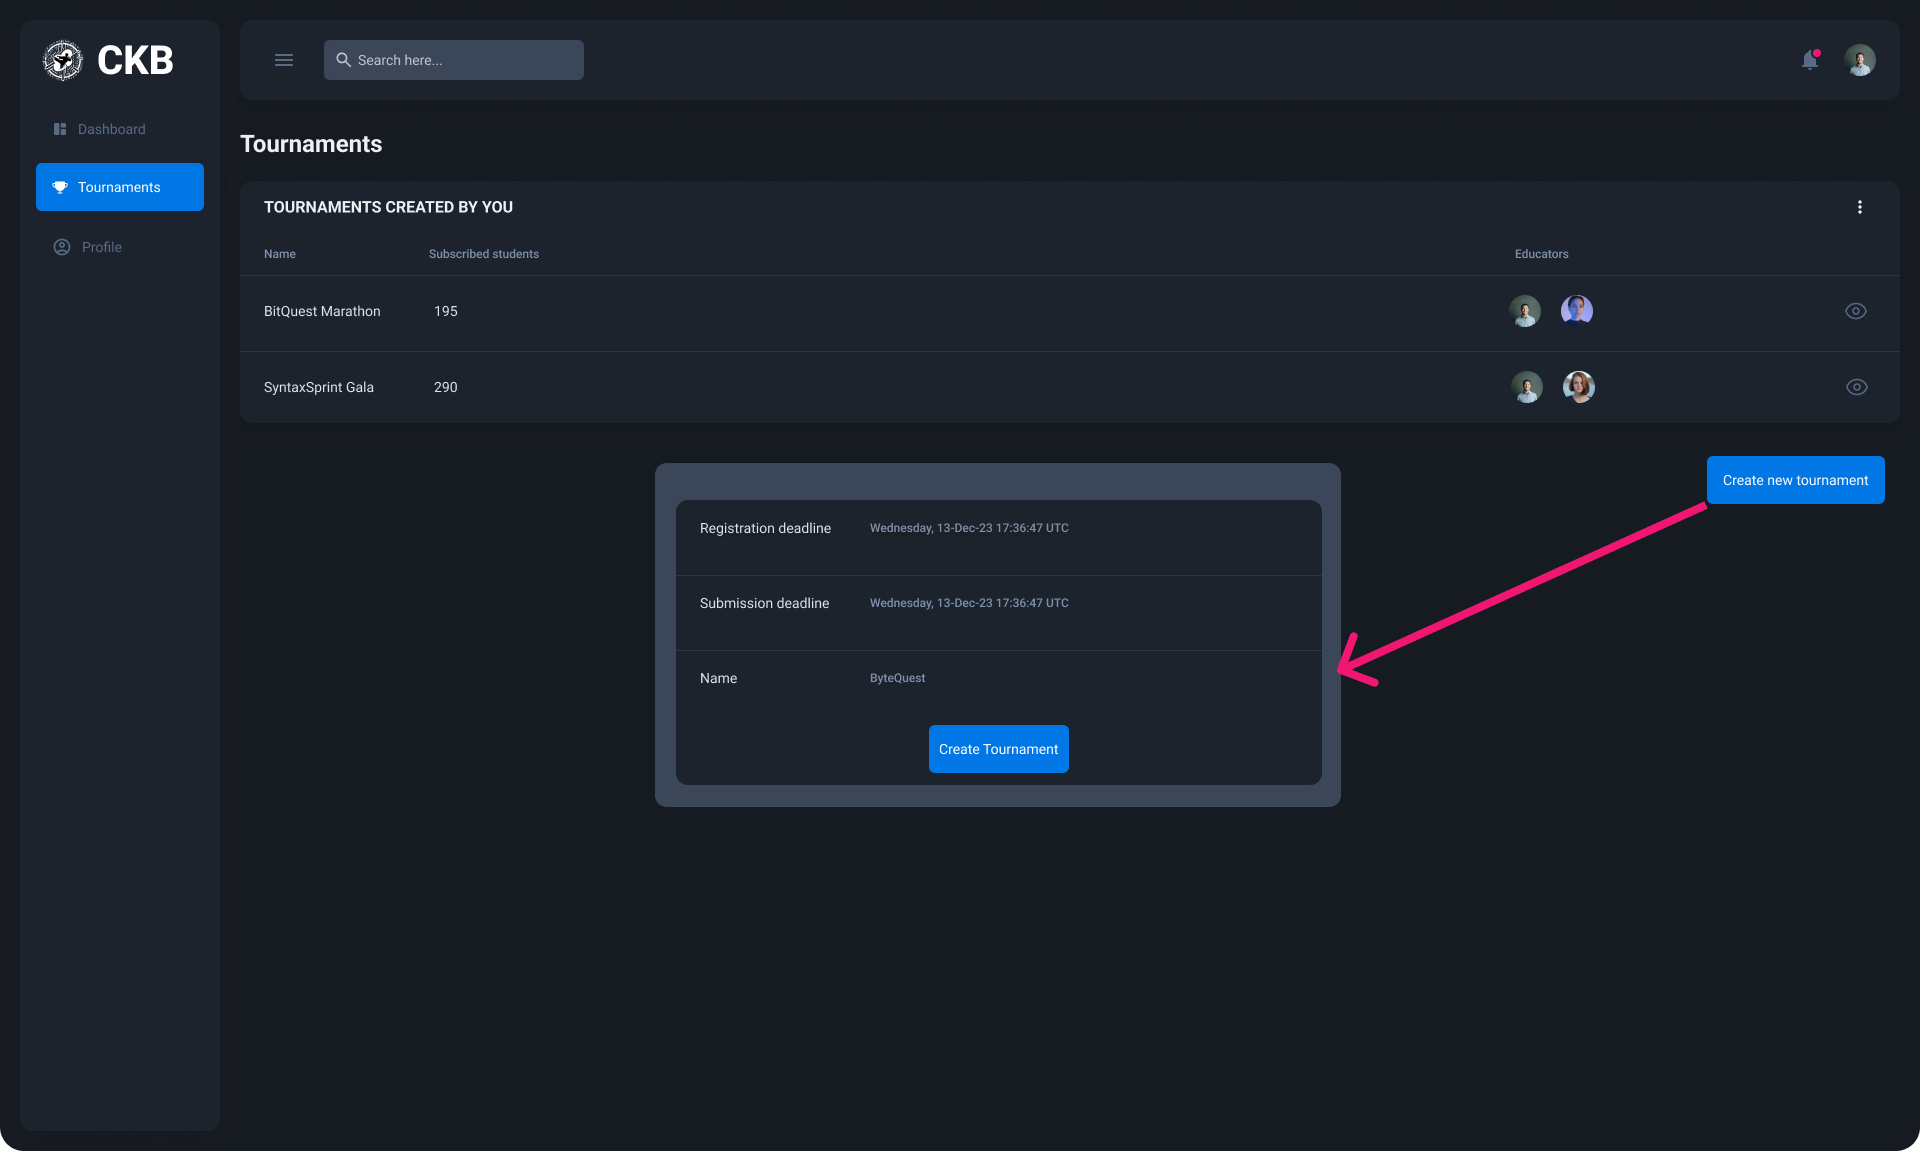
\includegraphics[width=\textwidth]{Images/TournamentCreationEducator.png}
    \caption{Educator Tournament Creation}
    \label{fig:student-Tournament-Completed}
\end{figure}

\begin{figure}[H]
    \centering
    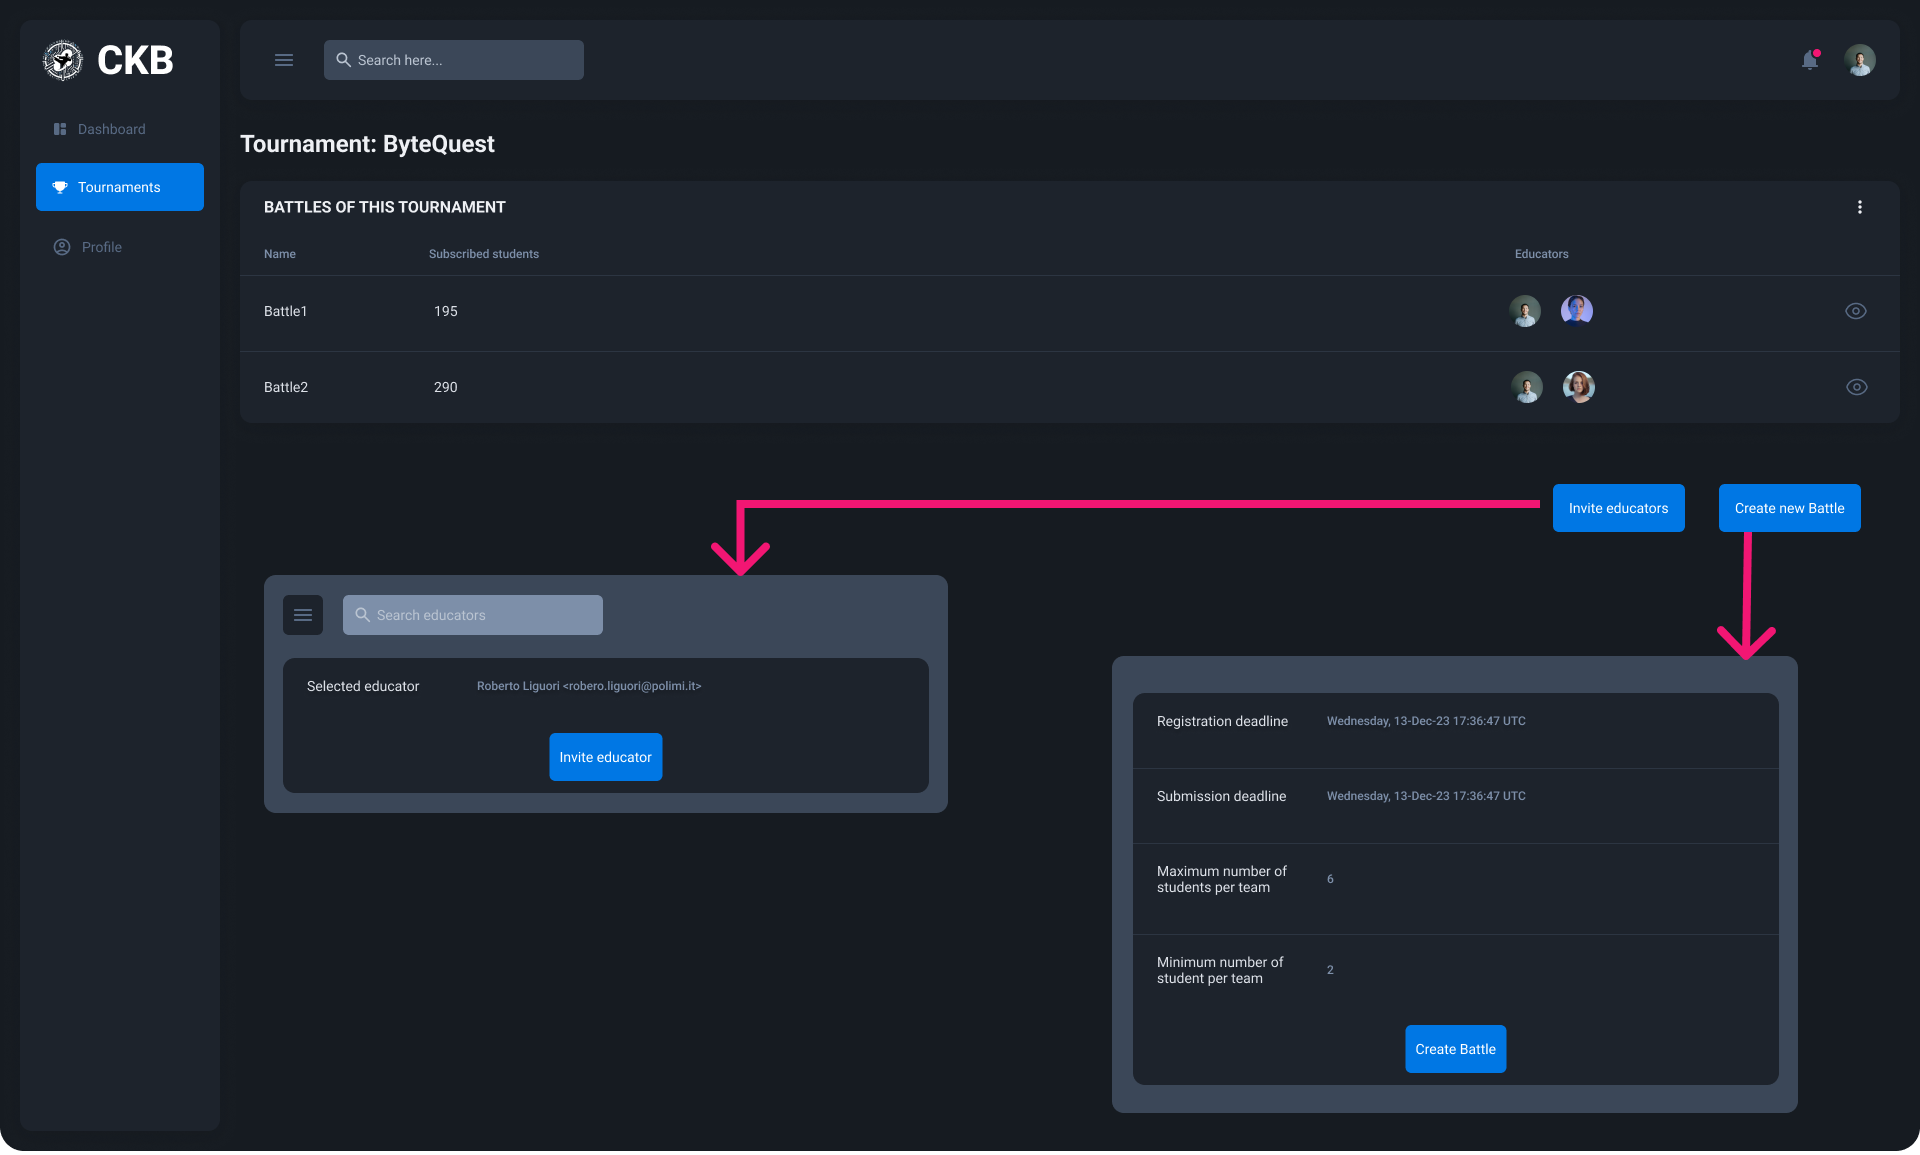
\includegraphics[width=\textwidth]{Images/BattleEducator.png}
    \caption{Educator Battle Creation and Educator invitation}
    \label{fig:student-Tournament-Completed}
\end{figure}

\begin{figure}[H]
    \centering
    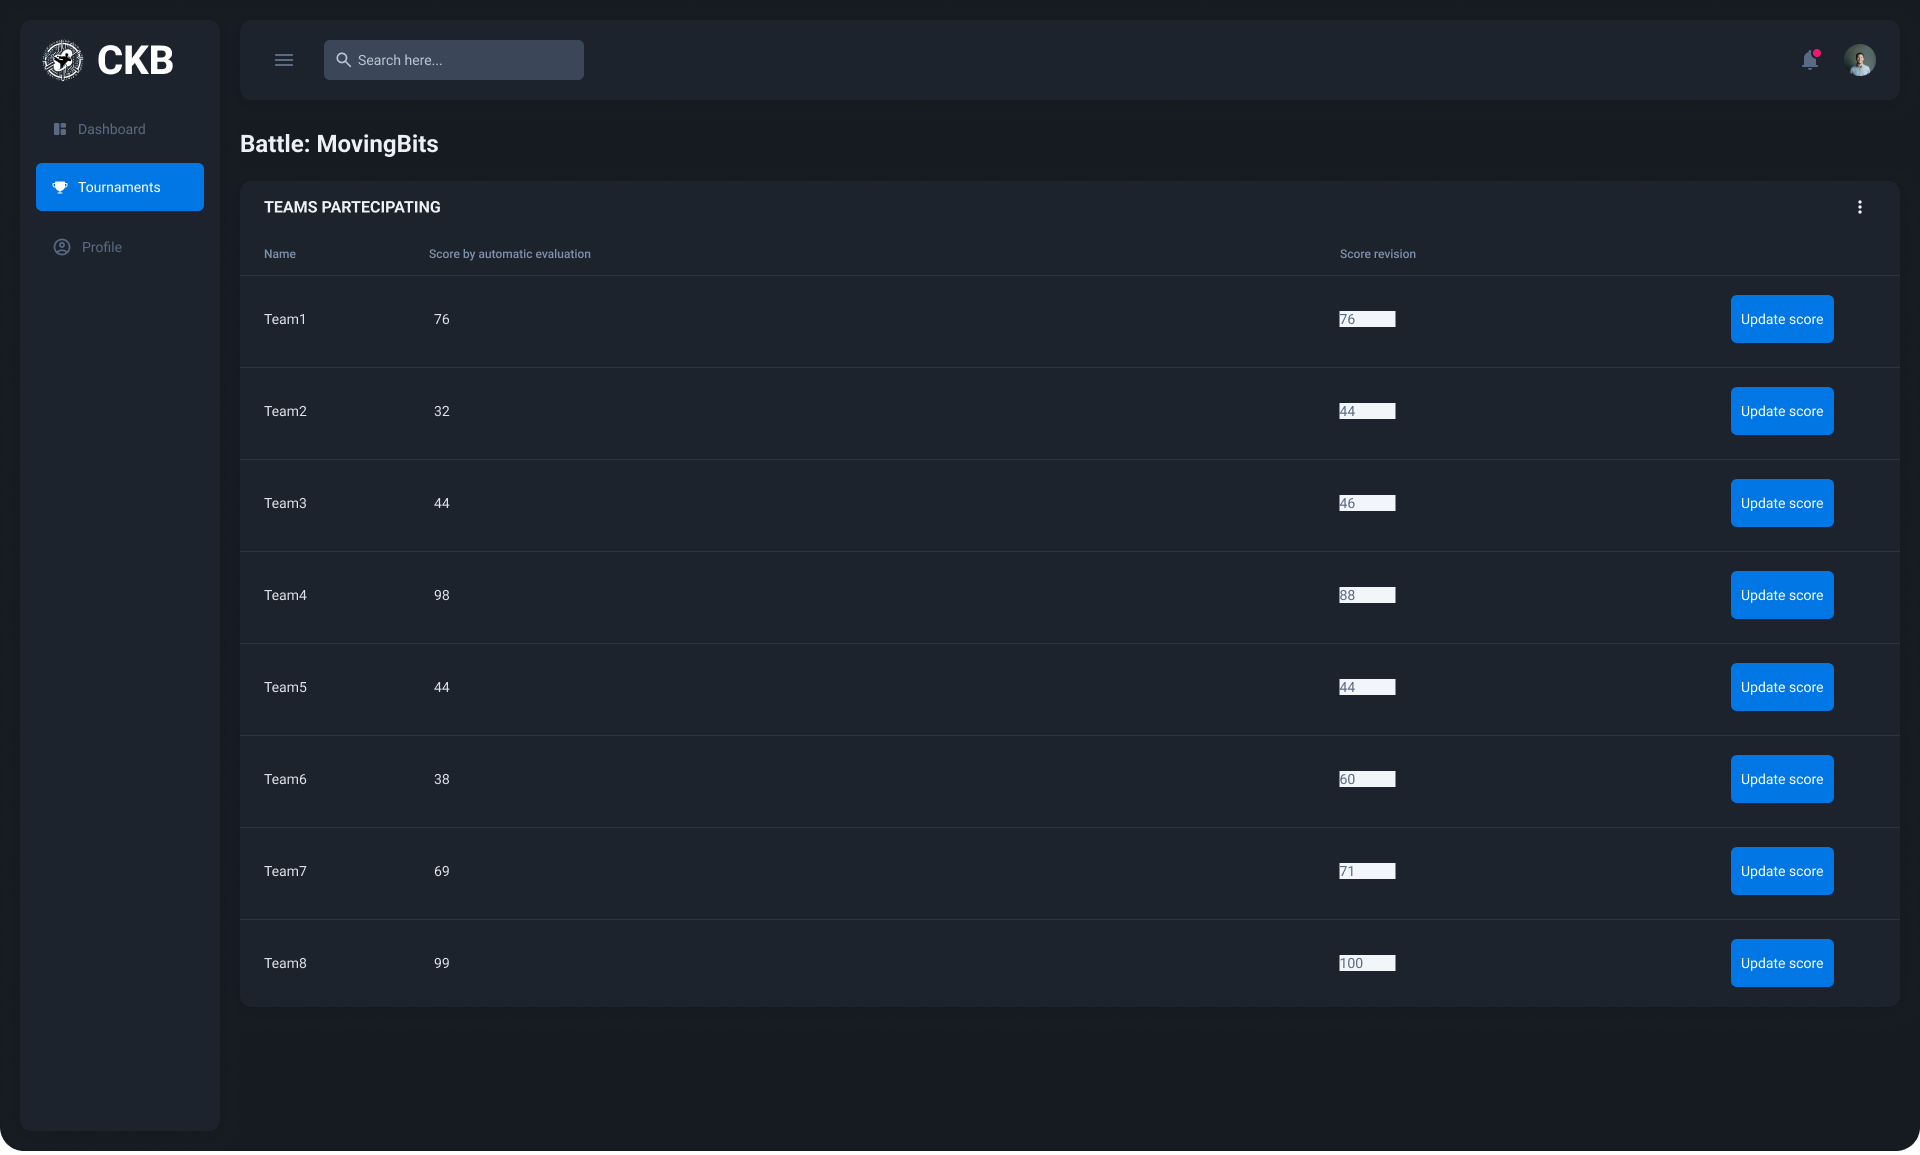
\includegraphics[width=\textwidth]{Images/ManualScoreUpdateEducator.png}
    \caption{Educator Manual Score Update for a battle}
    \label{fig:student-Tournament-Completed}
\end{figure}

\subsubsection{Hardware Interfaces}
Since there is no particular hardware requirement for the system, the system will be able to run on any hardware that can run a web browser and has an internet connection.

\subsubsection{Software Interfaces}
The system will utilize the GitHub API to streamline its operations. It will be used to create repository by CKB Platform and to trigger real-time evaluations of submissions. This approach ensures efficient management and transparent, interactive engagement for participants directly within their GitHub environment.

\subsubsection{Communication Interfaces}
The system provides the functionality of automatic evaluation. This function requires the system to communicate with an external client that triggers this automatic actions. In particular, the system needs to expose an API that the GitHub Action set up by the students will call when a new commit is pushed.

\subsection{Functional Requirements}
This section specifies all the requirements that the system must satisfy in order to be considered complete and functional.

\begin{enumerate}[label=R\arabic*:]
    \item The system shall allow the user to register to the system
    \item The system shall allow the user to login to the system
    \item The system shall allow the educator to create a new tournament
    \item The system should allow the educator to create a new battle for a tournament
    \item The system shall allow the educator to set restrictions for a battle
    \item The system shall allow the educator to upload the code kata for a battle
    \item The system shall allow the student to subscribe to a tournament
    \item The system shall allow the student to subscribe to a battle
    \item The system shall create a repository for each battle such that is forkable by the students
    \item The system shall allow the student to create a team for a battle
    \item The system should allow the student to invite other students to join a team
    \item The system should notify students subscribed to the platform when a new tournament is created
    \item The system should notify students subscribed to a tournament when a new battle is created
    \item The system should notify students subscribed to a tournament when the system publishes the ranking of the tournament
    \item The system shall guarantee that the restrictions for a battle set by the educator are respected
    \item The system shall allow the educator that created a tournament to invite other educators to the tournament
    \item The system shall allow the educator to close a tournament
    \item The system should allow the educator to manually update the score of a team for a battle
    \item The system should allow GitHub to trigger the automatic evaluation of a submission
\end{enumerate}

\subsubsection{Use Cases Diagram}
\subsubsection*{Educator Use Diagram}
\begin{figure}[H]
    \centering
    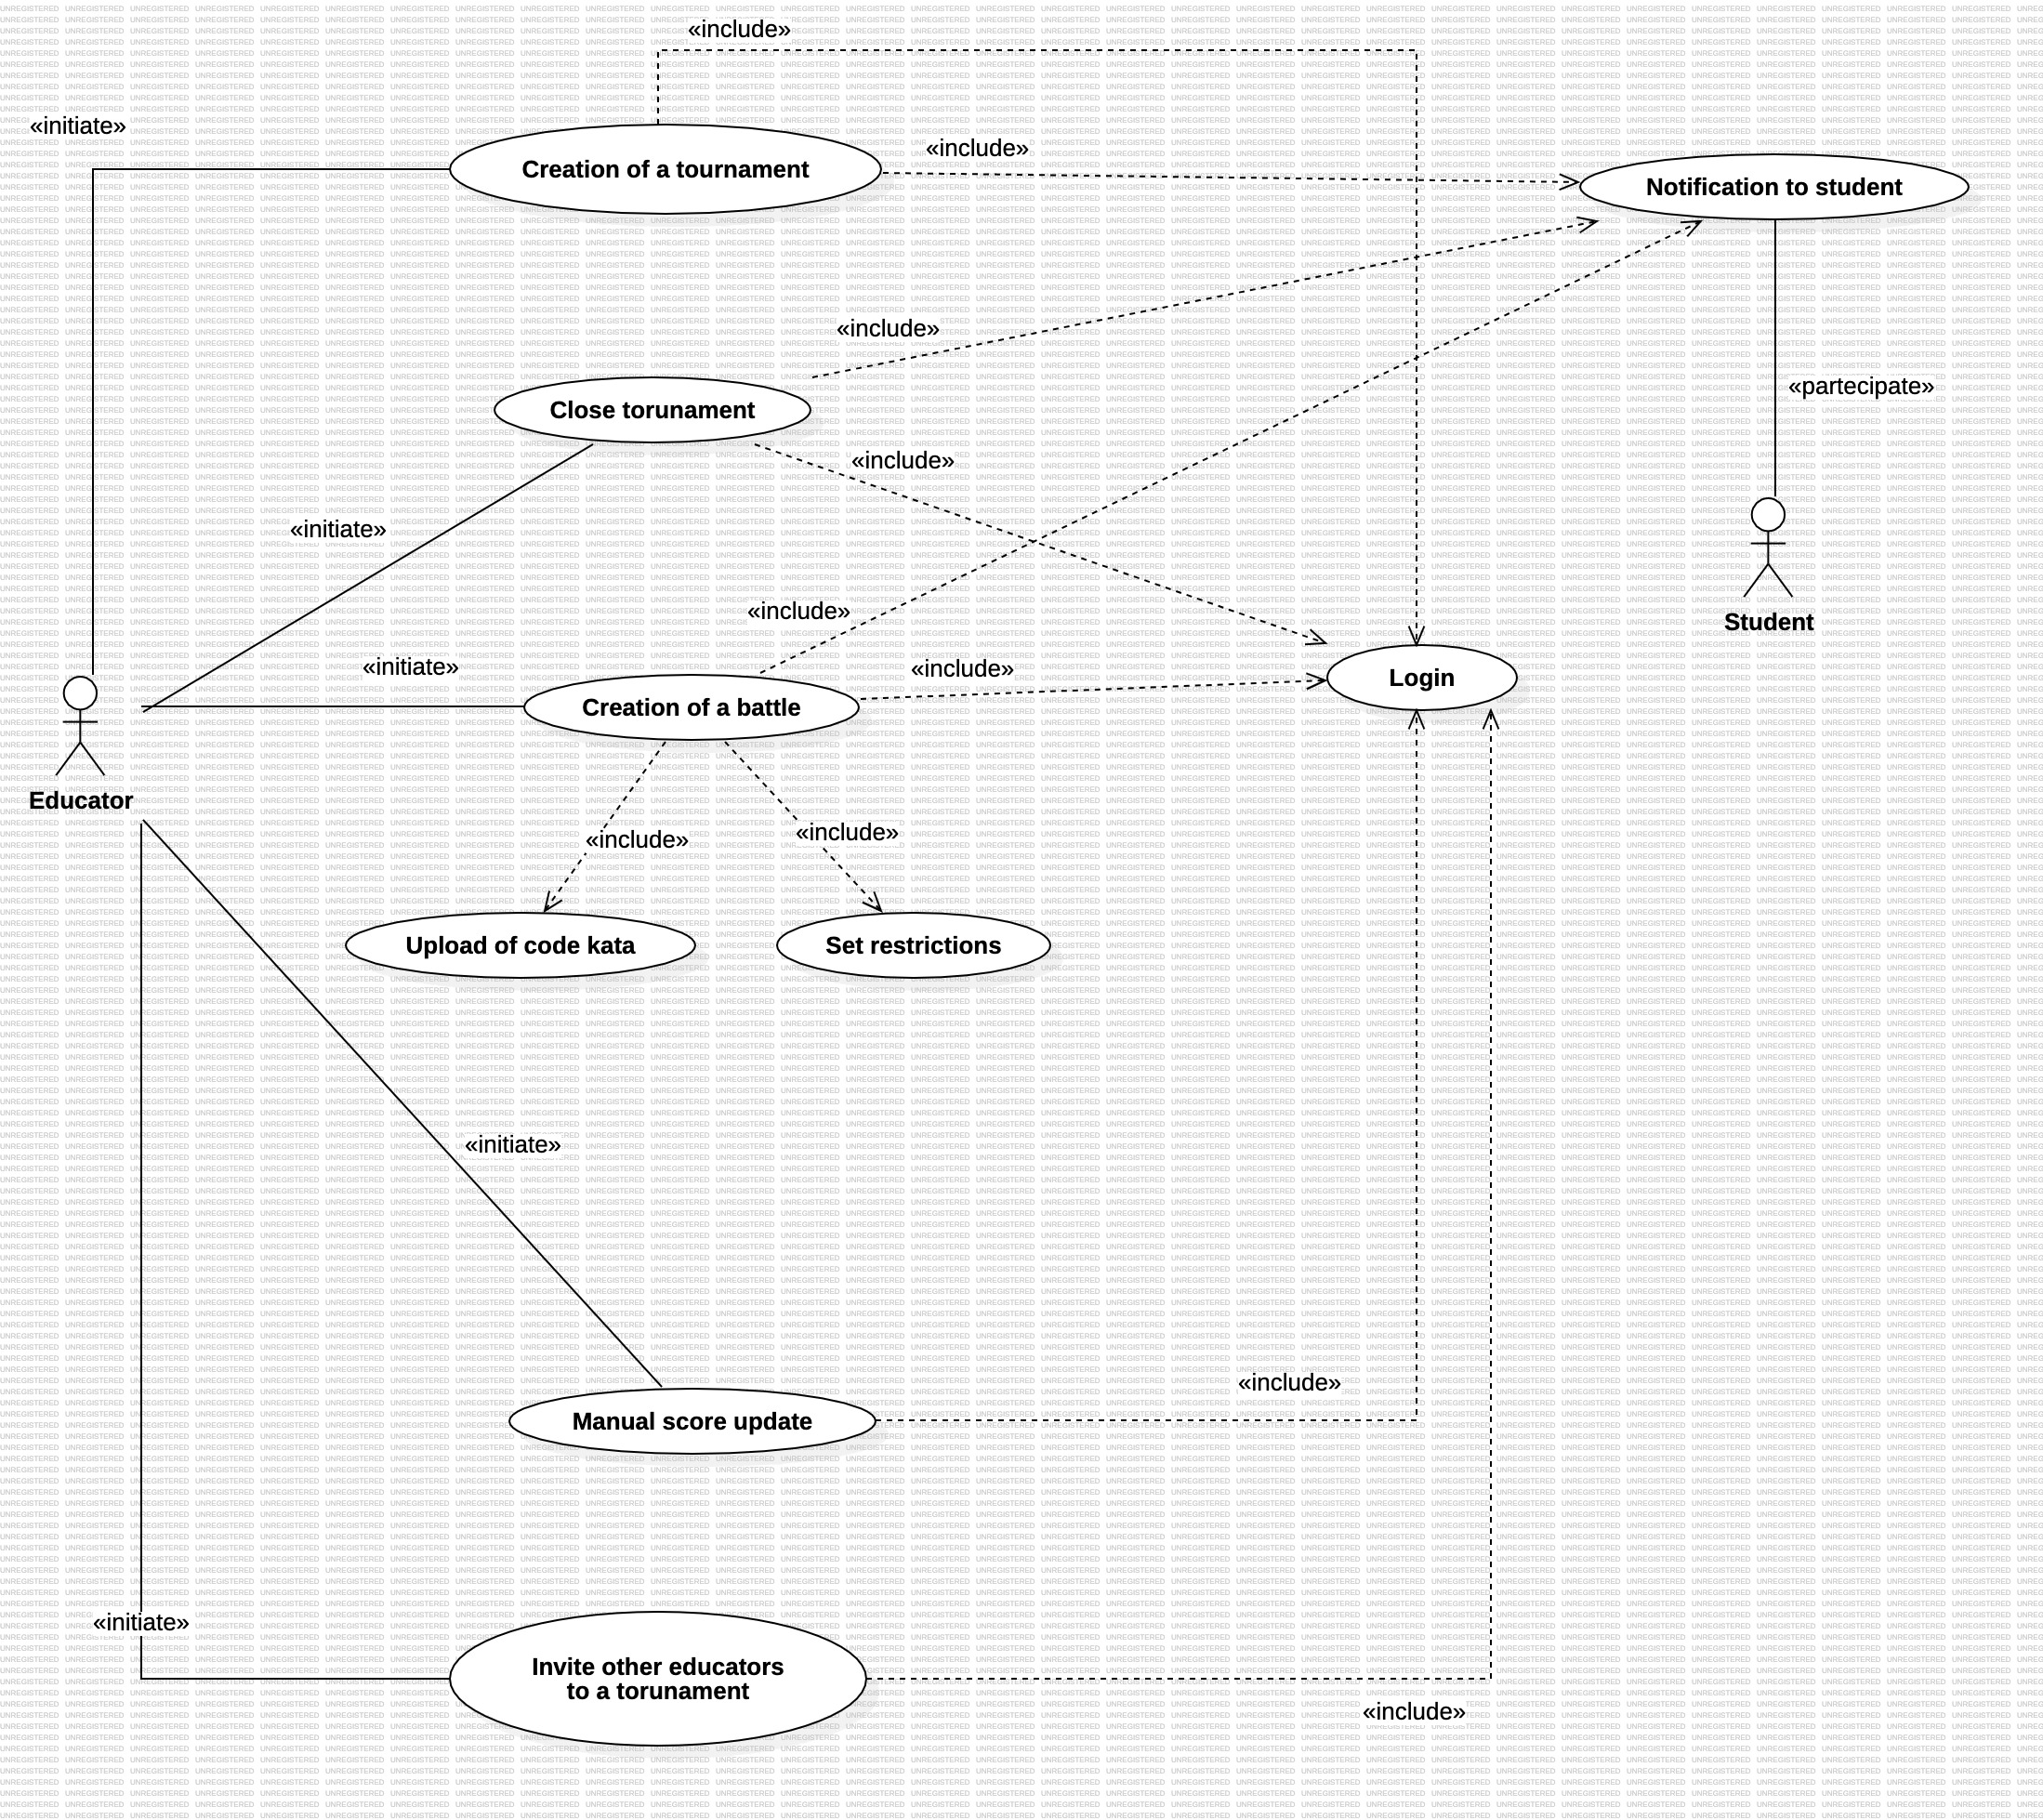
\includegraphics[width=\textwidth]{Diagrams/EducatorUseCaseDiagram.jpg}
    \caption{Educator Use Cases Diagram}
    \label{fig:student-use-diagram}
\end{figure}

\subsubsection*{Student Use Diagram}
\begin{figure}[H]
    \centering
    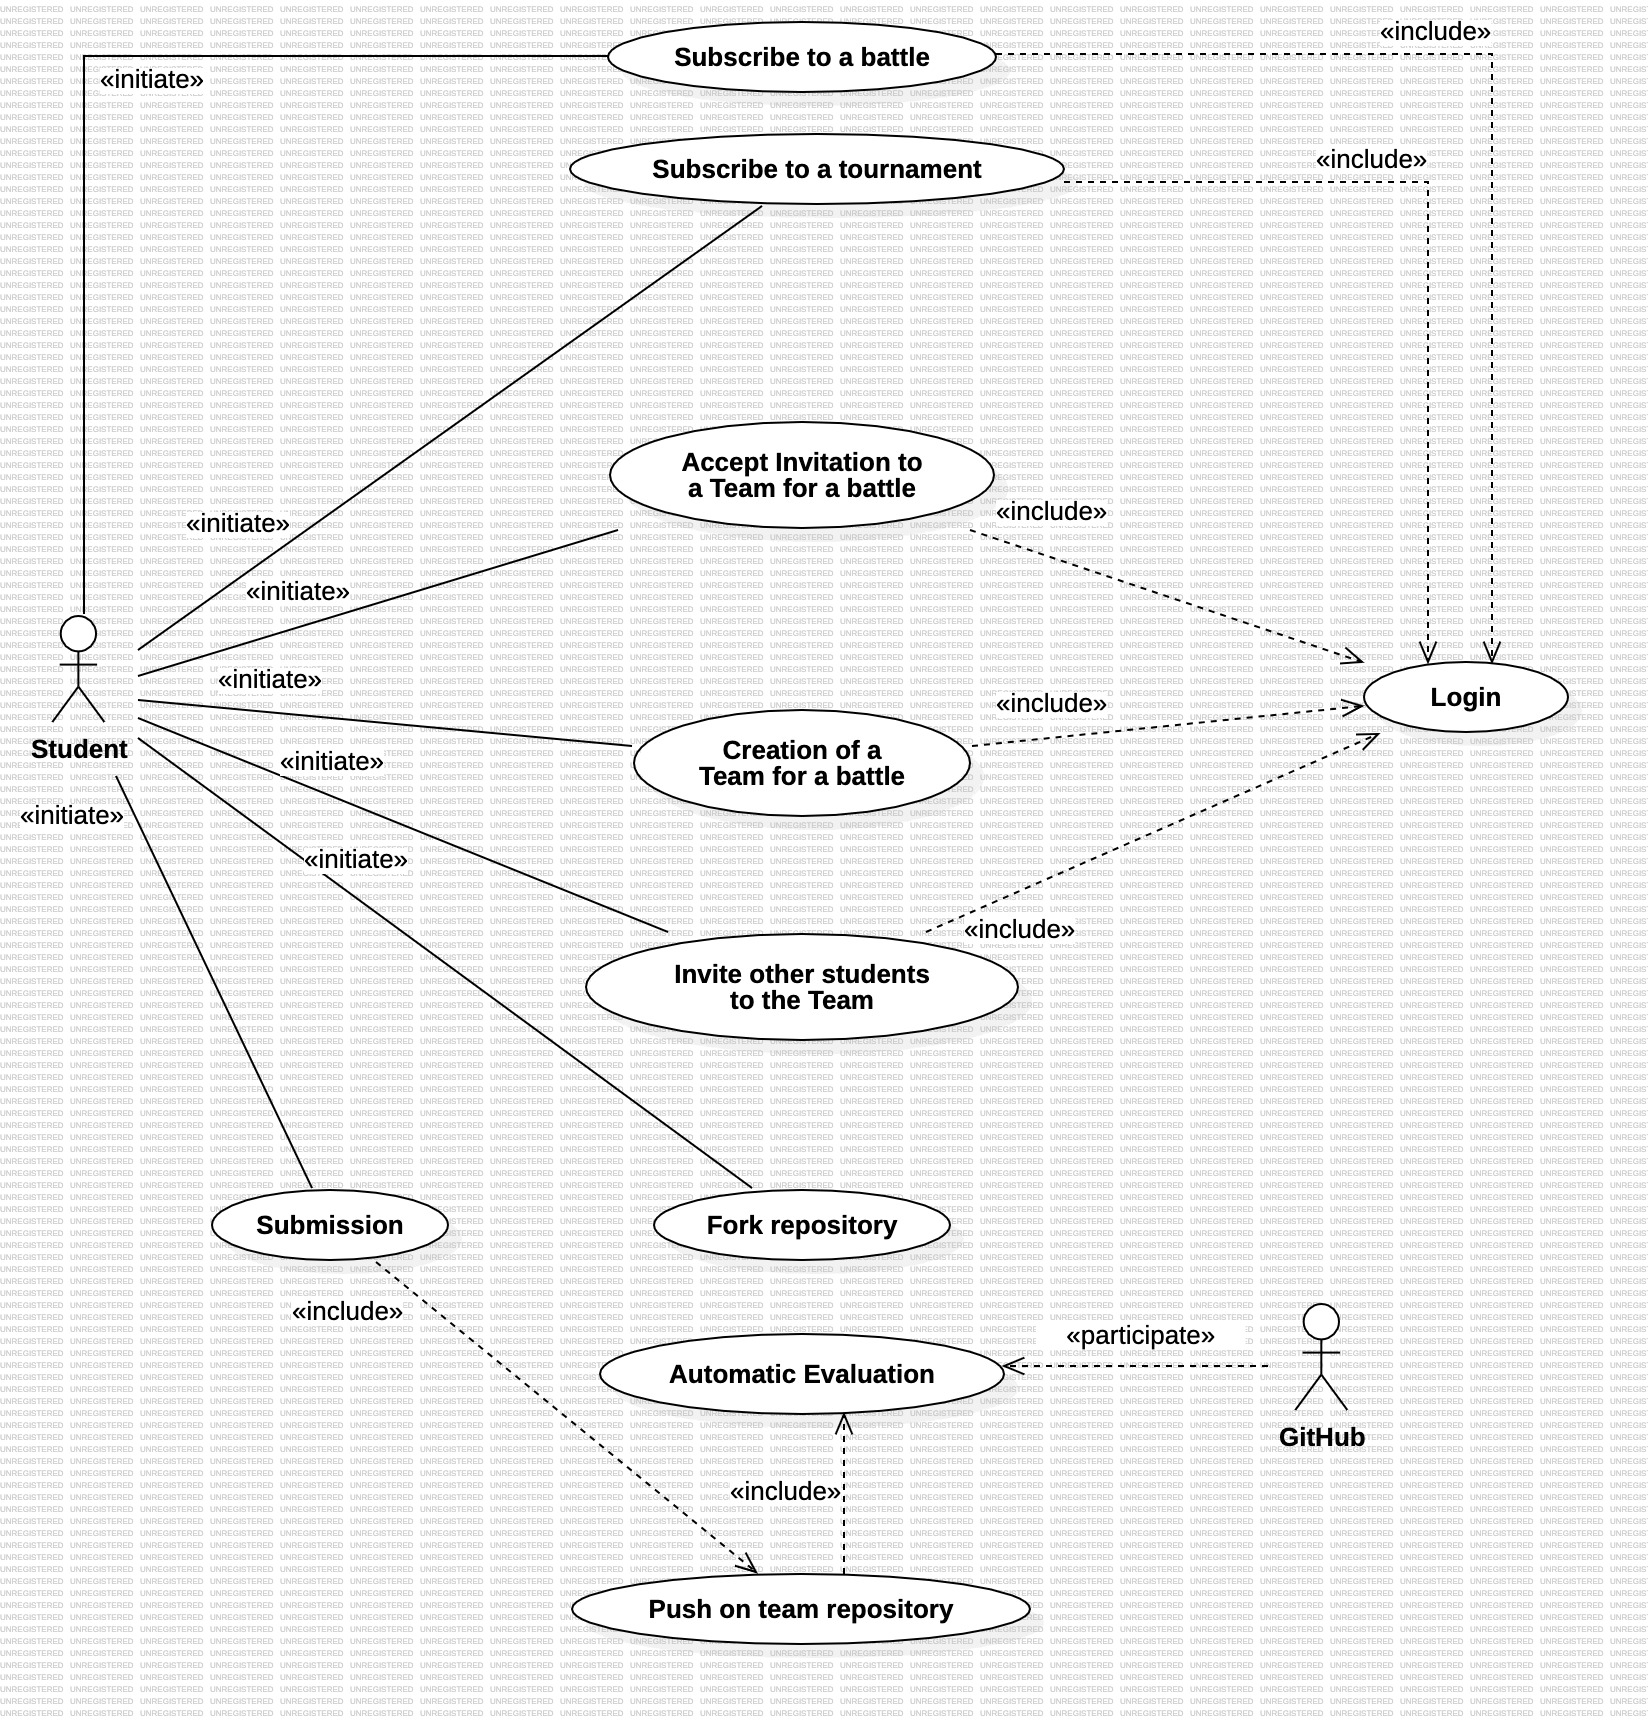
\includegraphics[width=\textwidth]{Diagrams/StudentUseCaseDiagram.jpg}
    \caption{Student Use Cases Diagram}
    \label{fig:student-use-diagram}
\end{figure}

\subsubsection{Use Cases}
\begin{enumerate}[label=UC\arabic*:]
    \item \textbf{User Login} \\
    \begin{tabular}{|p{3cm}|p{8cm}|}
        \hline
        Name & User Login \\
        \hline
        Actors & User \\
        \hline
        Entry condition & 
        \begin{itemize}
            \item The user is not logged in
            \item The user is registered to the system
            \item The user has a valid email and password
            \item The user has confirmed his email
        \end{itemize} 
        \\
        \hline
        Event flow &
        \begin{enumerate}[label=\arabic*.]
            \item The user enters his email and password
            \item The user clicks on the `Login' button
            \item The system checks the credentials
            \item The system logs in the user
            \item The user is redirected to the dashboard
        \end{enumerate}
        \\
        \hline
        Exit condition & 
        \begin{itemize}
            \item The user is logged in
        \end{itemize}
        \\
        \hline
        Exceptions &
        \begin{itemize}
            \item The user enters an invalid email or password
            \item The user has not confirmed his email
            \item The user is not registered to the system
        \end{itemize}
        \\
        \hline
    \end{tabular}
    \item \textbf{Creation of a tournament} \\
    \begin{tabular}{|p{3cm}|p{8cm}|}
        \hline
        Name & Creation of a tournament \\
        \hline
        Actors & Educator, Student \\
        \hline
        Entry condition &
        \begin{itemize}
            \item The Educator is subscribed to CKB platform
            \item The Student is subscribed to CKB platform
        \end{itemize}
        \\
        \hline
        Event flow & 
        \begin{enumerate}[label=\arabic*.]
            \item The Educator logs in to the system
            \item The Educator clicks on the `Create Tournament button
            \item The Educator fills the form with the information about the tournament, the registration deadline and the starting date
            \item The Educator clicks on the `Create button
            \item The system creates the tournament
            \item The system notifies the subscribed students about the creation of the new tournament
        \end{enumerate}
        \\
        \hline
        Exit condition & The Educator successfully created the torunament \\
        \hline
    \end{tabular}
    \item \textbf{Close a tournament} \\
    \begin{tabular}{|p{3cm}|p{8cm}|}
    \hline
    Name & Close a tournament \\
    \hline
    Actors & Educator, Student \\
    \hline
    Entry condition &
    \begin{itemize}
        \item The Educator is subscribed to CKB platform
        \item The Educator created a tournament
        \item The registration deadline of the tournament is passed
        \item The tournament is not closed
    \end{itemize}
    \\
    \hline
    Event flow &
    \begin{enumerate}[label=\arabic*.]
        \item The Educator logs in to the system
        \item The Educator goes to the tournament page in which he wants to close
        \item The Educator clicks on the `Close Tournament' button
        \item The system closes the tournament
        \item The system notifies the subscribed students about the closing of the tournament
    \end{enumerate}
    \\
    \hline
    Exit condition & The Educator successfully closed the tournament \\
    \hline
    Exceptions & The registration deadline of the tournament is not passed \\
    \hline
    \end{tabular}
    \item \textbf{Creation of a battle} \\
    \begin{tabular}{|p{3cm}|p{8cm}|}
        \hline
        Name & Creation of a battle \\
        \hline
        Actors & Educator, Student, GitHub \\
        \hline
        Entry condition &
        \begin{itemize}
            \item The Educator is subscribed to CKB platform
            \item The Student is subscribed to CKB platform
            \item The Educator created a tournament
            \item The Student is subscribed to the tournament
        \end{itemize}
        \\
        \hline
        Event flow & 
        \begin{enumerate}[label=\arabic*.]
            \item The Educator logs in to the system
            \item The Educator goes to the tournament page in which he wants to create a battle for
            \item The Educator clicks on the `Create Battle button
            \item The Educator fills the form with the registration deadline, submission deadline, minimum number of students per team, maximum number of students per team
            \item The Educator click the `Upload Code Kata' button and selects the files to upload
            \item The Educator clicks on the `Create button
            \item The system creates the battle
            \item GitHub creates a forkable repository for the battle
            \item The system sends the link of the repository to the subscribed students
            \item The system notifies the subscribed students about the creation of the new battle
        \end{enumerate}
        \\
        \hline
        Exit condition & The Educator successfully created the battle \\
        \hline
    \end{tabular}
    \item \textbf{Upload of code kata} \\
    \begin{tabular}{|p{3cm}|p{8cm}|}
        \hline
        Name & Upload of code kata \\
        \hline
        Actors & Educator \\
        \hline
        Entry condition &
        \begin{itemize}
            \item The Educator is subscribed to CKB platform
            \item The Educator is logged in
            \item The Educator created a tournament
            \item The Educator created a battle for the tournament
        \end{itemize}
        \\
        \hline
        Event flow &
        \begin{enumerate}[label=\arabic*.]
            \item The Educator goes to the tournament page in which he wants to upload the code kata
            \item The Educator selects the battle in which he wants to upload the code kata
            \item The Educator clicks on the `Upload Code Kata' button
            \item The Educator selects the files to upload
            \item The Educator clicks on the `Upload' button
            \item The system uploads the code kata
        \end{enumerate}
        \\
        \hline
        Exit condition & The code kata is uploaded \\
        \hline
        Exceptions & The Educator is not the creator of the tournament \\
        \hline
    \end{tabular}
    \item \textbf{Manual score update} \\
    \begin{tabular}{|p{3cm}|p{8cm}|}
        \hline
        Name & Manual score update \\
        \hline
        Actors & Educator \\
        \hline
        Entry condition &   
        \begin{itemize}
            \item The Educator is subscribed to CKB platform
            \item The Educator is logged in
            \item The Educator created a tournament
            \item The Educator created a battle for the tournament
        \end{itemize}
        \\
        \hline
        Event flow &
        \begin{enumerate}[label=\arabic*.]
            \item The Educator goes to the tournament page in which he wants to update the score
            \item The Educator selects the battle in which he wants to update the score
            \item The Educator clicks on the `Update Score' button
            \item The Educator selects the team for which he wants to update the score
            \item The Educator fills the form with the new score
            \item The Educator clicks on the `Update' button
        \end{enumerate}
        \\
        \hline
        Exit condition & The score is updated \\
        \hline
        Exceptions & The Educator is not the creator of the tournament \\
        \hline
    \end{tabular}
    \item \textbf{Invite other educators to a tournament} \\
    \begin{tabular}{|p{3cm}|p{8cm}|}
        \hline
        Name & Invite other educators to a tournament \\
        \hline
        Actors & Educator \\
        \hline
        Entry condition &
        \begin{itemize}
            \item The Educator is subscribed to CKB platform
            \item The Educator created a tournament
        \end{itemize}
        \\
        \hline
        Event flow & 
        \begin{enumerate}[label=\arabic*.]
            \item The Educator logs in to the system
            \item The Educator goes to the tournament page in which he wants to invite other educators
            \item The Educator clicks on the `Invite Educator' button
            \item The Educator fills the form with the email of the educator to invite
            \item The Educator clicks on the `Invite' button
            \item The system sends an email to the educator to invite
        \end{enumerate}
        \\
        \hline
        Exit condition &
        \begin{itemize}
            \item The Educator successfully invited the other educator to the tournament
            \item The invited educator can create battles for the tournament
        \end{itemize} \\
        \hline
        Exceptions & The invited educator is not subscribed to the platform \\
        \hline
    \end{tabular}
    \item \textbf{Notification to a student} \\
    \begin{tabular}{|p{3cm}|p{8cm}|}
        \hline
        Name & Notification to a student \\
        \hline
        Actors & Educator, Student \\
        \hline
        Entry condition &
        \begin{itemize}
            \item The Student is subscribed to CKB platform
        \end{itemize}
        \\
        \hline
        Event flow &
        \begin{enumerate}[label=\arabic*.]
            \item The Educator creates or closes a tournament or a battle
            \item The system notifies the subscribed students about the event
        \end{enumerate}
        \\
        \hline
        Exit condition & The student has received the notification   \\
        \hline
    \end{tabular}
    \item \textbf{Subscribe to a tournament} \\
    \begin{tabular}{|p{3cm}|p{8cm}|}
        \hline
        Name & Student subscribe to a tournament \\
        \hline
        Actors & Student \\
        \hline
        Entry condition &
        \begin{itemize}
            \item The Student is subscribed to CKB platform
            \item The Educator created a tournament
            \item The Student is not subscribed to the tournament
        \end{itemize}
        \\
        \hline
        Event flow &
        \begin{enumerate}[label=\arabic*.]
            \item The Student logs in to the system
            \item The Student goes to the tournament page in which he wants to subscribe
            \item The Student clicks on the `Subscribe' button
        \end{enumerate} \\
        \hline
        Exit condition & The student is subscibed to the tournament \\
        \hline
        Exceptions & The registration deadline of the tournament is passed so
        the student cannot subscribe to the tournament \\
        \hline
    \end{tabular}
    \item \textbf{Subscribe to a battle} \\
    \begin{tabular}{|p{3cm}|p{8cm}|}
        \hline
        Name & Student subscribe to a battle \\
        \hline
        Actors & Student \\
        \hline
        Entry condition &
        \begin{itemize}
            \item The Student is subscribed to CKB platform
            \item The Student is subscribed to the tournament in which the battle is
            \item The Student is not subscribed to the battle
        \end{itemize}
        \\
        \hline
        Event flow &
        \begin{enumerate}[label=\arabic*.]
            \item The Student logs in to the system
            \item The Student goes to the tournament page
            \item The Student selects the battle in which he wants to subscribe
            \item The Student clicks on the `Subscribe' button
        \end{enumerate} \\
        \hline
        Exit condition & The student is subscibed to the battle \\
        \hline
        Exceptions & The registration deadline of the battle is passed so the student cannot subscribe to the battle \\
        \hline
    \end{tabular}
    \item \textbf{Accept invitation to a team for a battle} \\
    \begin{tabular}{|p{3cm}|p{8cm}|}
        \hline
        Name & Accept invitation to a team for a battle \\
        \hline
        Actors & Student \\
        \hline
        Entry condition &
        \begin{itemize}
            \item The Student is subscribed to CKB platform
            \item The Student is subscribed to the tournament in which the battle is
            \item The Student is subscribed to the battle
            \item The Student is not in a team for the battle
        \end{itemize} \\
        \hline
        Event flow &
        \begin{enumerate}[label=\arabic*.]
            \item The Student logs in to the system
            \item The Student goes to the notification page
            \item The Student clicks on the `Accept Invitation' button
            \item The system adds the student to the team for the battle
        \end{enumerate} \\
        \hline
        Exit condition & The invited student is part of the team for the battle \\
        \hline
        Exceptions &
        \begin{itemize}
            \item The submission deadline of the battle is passed so the student cannot subscribe to the battle
            \item The maximum number of students per team is reached so the student cannot subscribe to the Battle
            \item The invitation is expired so the student cannot subscribe to the battle
        \end{itemize} \\
        \hline
    \end{tabular}
    \item \textbf{Creation of a team for a battle} \\
    \begin{tabular}{|p{3cm}|p{8cm}|}
        \hline
        Name & Creation of a team for a battle \\
        \hline
        Actors & Student \\
        \hline
        Entry condition &
        \begin{itemize}
            \item The Student is subscribed to CKB platform
            \item The Student is subscribed to the tournament in which the battle is
            \item The Student is subscribed to the battle
            \item The Student is not in a team for the battle
        \end{itemize} \\
        \hline
        Event flow &
        \begin{enumerate}[label=\arabic*.]
            \item The Student logs in to the system
            \item The Student goes to the tournament page
            \item The Student selects the battle in which he wants to create a team
            \item The Student clicks on the `Create Team' button
            \item The Student fills the form with the name of the team
            \item The Student clicks on the `Create' button
        \end{enumerate} \\
        \hline
        Exit condition & The student is part of the team for the battle \\
        \hline
        Exceptions & The submission deadline of the battle is passed so the student cannot subscribe to the battle \\
        \hline
    \end{tabular}
    \item \textbf{Invite other students to the team} \\
    \begin{tabular}{|p{3cm}|p{8cm}|}
        \hline
        Name & Invite other students to the team \\
        \hline
        Actors & Student \\
        \hline
        Entry condition &
        \begin{itemize}
            \item The Student is subscribed to CKB platform
            \item The Student is subscribed to the tournament in which the battle is
            \item The Student is subscribed to the battle
        \end{itemize} \\
        \hline
        Event flow &
        \begin{enumerate}[label=\arabic*.]
            \item The Student logs in to the system
            \item The Student goes to the tournament page
            \item The Student selects the battle in which he wants to invite other students
            \item The Student clicks on the `Invite people' button
            \item The Student fills the form with the email of the students to invite
            \item The Student clicks on the `Invite' button
        \end{enumerate} \\
        \hline
        Exit condition & The student has been successfully invited to the team \\
        \hline
        Exceptions & The student invited is not registered on the CKB platform so he will not receive the invitation \\
        \hline
    \end{tabular}
    \item \textbf{Fork repository of a battle} \\
    \begin{tabular}{|p{3cm}|p{8cm}|}
        \hline
        Name & Fork repository of a battle \\
        \hline
        Actors & Student \\
        \hline
        Entry condition &
        \begin{itemize}
            \item The Student is subscribed to CKB platform
            \item The Student is subscribed to the tournament in which the battle is
            \item The Student is subscribed to the battle
        \end{itemize} \\
        \hline
        Event flow &
        \begin{enumerate}[label=\arabic*.]
            \item The Student logs in to the system
            \item The Student goes to the tournament page
            \item The Student selects the battle in which he wants to fork the repository
            \item The Student clicks on the `Repository' button
            \item The system redirects the Student to the GitHub page of the repository to fork
        \end{enumerate} \\
        \hline
        Exit condition & The student has forked the repository \\
        \hline
        Exceptions & The submission deadline of the battle is passed so the student cannot fork the repository \\
        \hline
    \end{tabular}
    \item \textbf{Submission of a solution for a battle} \\
    \begin{tabular}{|p{3cm}|p{8cm}|}
        \hline
        Name & Submission of a solution for a battle \\
        \hline
        Actors & Student, GitHub \\
        \hline
        Entry condition &
        \begin{itemize}
            \item The Student is subscribed to CKB platform
            \item The Student is subscribed to the tournament in which the battle is
            \item The Student is subscribed to the battle
            \item The Student is part of a team for the battle
            \item The Student has forked the repository of the battle
            \item The Student set up the GitHub Action to trigger the automatic evaluation
        \end{itemize} \\
        \hline
        Event flow &
        \begin{enumerate}[label=\arabic*.]
            \item The Student writes the solution for the battle
            \item The Student pushes the solution on the team repository
            \item GitHub triggers the automatic evaluation
            \item The system evaluates the solution
            \item The system updates the score of the team
        \end{enumerate} \\
        \hline
        Exit condition & The team has got a new score for the battle \\
        \hline
        Exceptions & The submission deadline of the battle is passed so the student submission is not evaluated \\
        \hline
    \end{tabular}
    \item \textbf{Push on team repository} \\
    \begin{tabular}{|p{3cm}|p{8cm}|}
        \hline
        Name & Push on team repository \\
        \hline
        Actors & Student, GitHub \\
        \hline
        Entry condition &
        \begin{itemize}
            \item The Student is subscribed to CKB platform
            \item The Student is subscribed to the tournament in which the battle is
            \item The Student is subscribed to the battle
            \item The Student is part of a team for the battle
            \item The Student has forked the repository of the battle
        \end{itemize} \\
        \hline
        Event flow &
        \begin{enumerate}[label=\arabic*.]
            \item The Student writes the solution for the battle
            \item The Student pushes the solution on the team repository
            \item GitHub triggers the automatic evaluation
            \item The system evaluates the solution
            \item The system updates the score of the team
        \end{enumerate} \\
        \hline
        Exit condition & The team has got a new score for the battle \\
        \hline
        Exceptions &
        \begin{itemize}
            \item The submission deadline of the battle is passed so the student submission is not evaluated
            \item The Student has not set up the GitHub Action to trigger the automatic evaluation
        \end{itemize} \\
        \hline
    \end{tabular}
    \item \textbf{Automatic evaluation of a submission} \\
    \begin{tabular}{|p{3cm}|p{8cm}|}
        \hline
        Name & Automatic evaluation of a submission \\
        \hline
        Actors & GitHub \\
        \hline
        Entry condition &
        \begin{itemize}
            \item The Student is subscribed to CKB platform
            \item The Student is subscribed to the tournament in which the battle is
            \item The Student is subscribed to the battle
            \item The Student is part of a team for the battle
            \item The Student has forked the repository of the battle
            \item The Student set up the GitHub Action to trigger the automatic evaluation
            \item The Student has pushed the solution on the team repository
        \end{itemize} \\
        \hline
        Event flow &
        \begin{enumerate}[label=\arabic*.]
            \item GitHub triggers the automatic evaluation
            \item The system builds the project with the building tool associated with the battle
            \item The system runs the tests associated with the battle on the built project
            \item The system calculate the score of the submission
        \end{enumerate} \\
        \hline
        Exit condition & The team has got a new score for the battle \\
        \hline
        Exceptions & The submission deadline of the battle is passed so the student submission is not evaluated \\
        \hline
    \end{tabular}
\end{enumerate}

\subsubsection{Sequence diagrams}
\subsubsection*{[UC1] Login}
\begin{figure}[H]
    \centering
    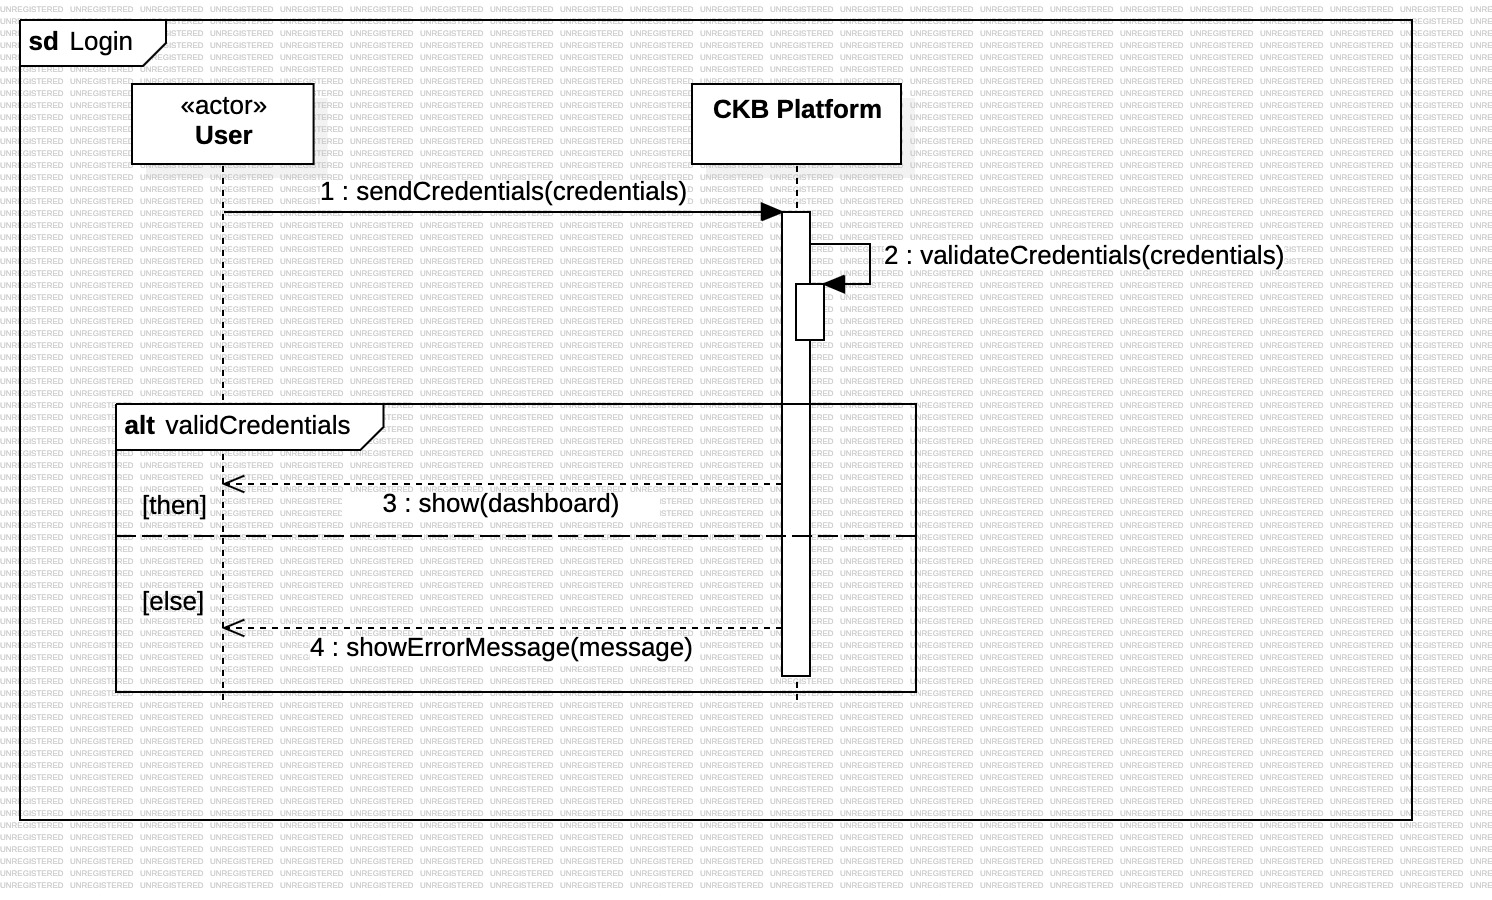
\includegraphics[width=\textwidth]{Diagrams/UC1SequenceDiagram.jpg}
    \caption{Sequence Diagram for the Login Use Case}
    \label{fig:sequence-diagram-login}
\end{figure}

\subsubsection*{[UC2] Creation of a tournament}
\begin{figure}[H]
    \centering
    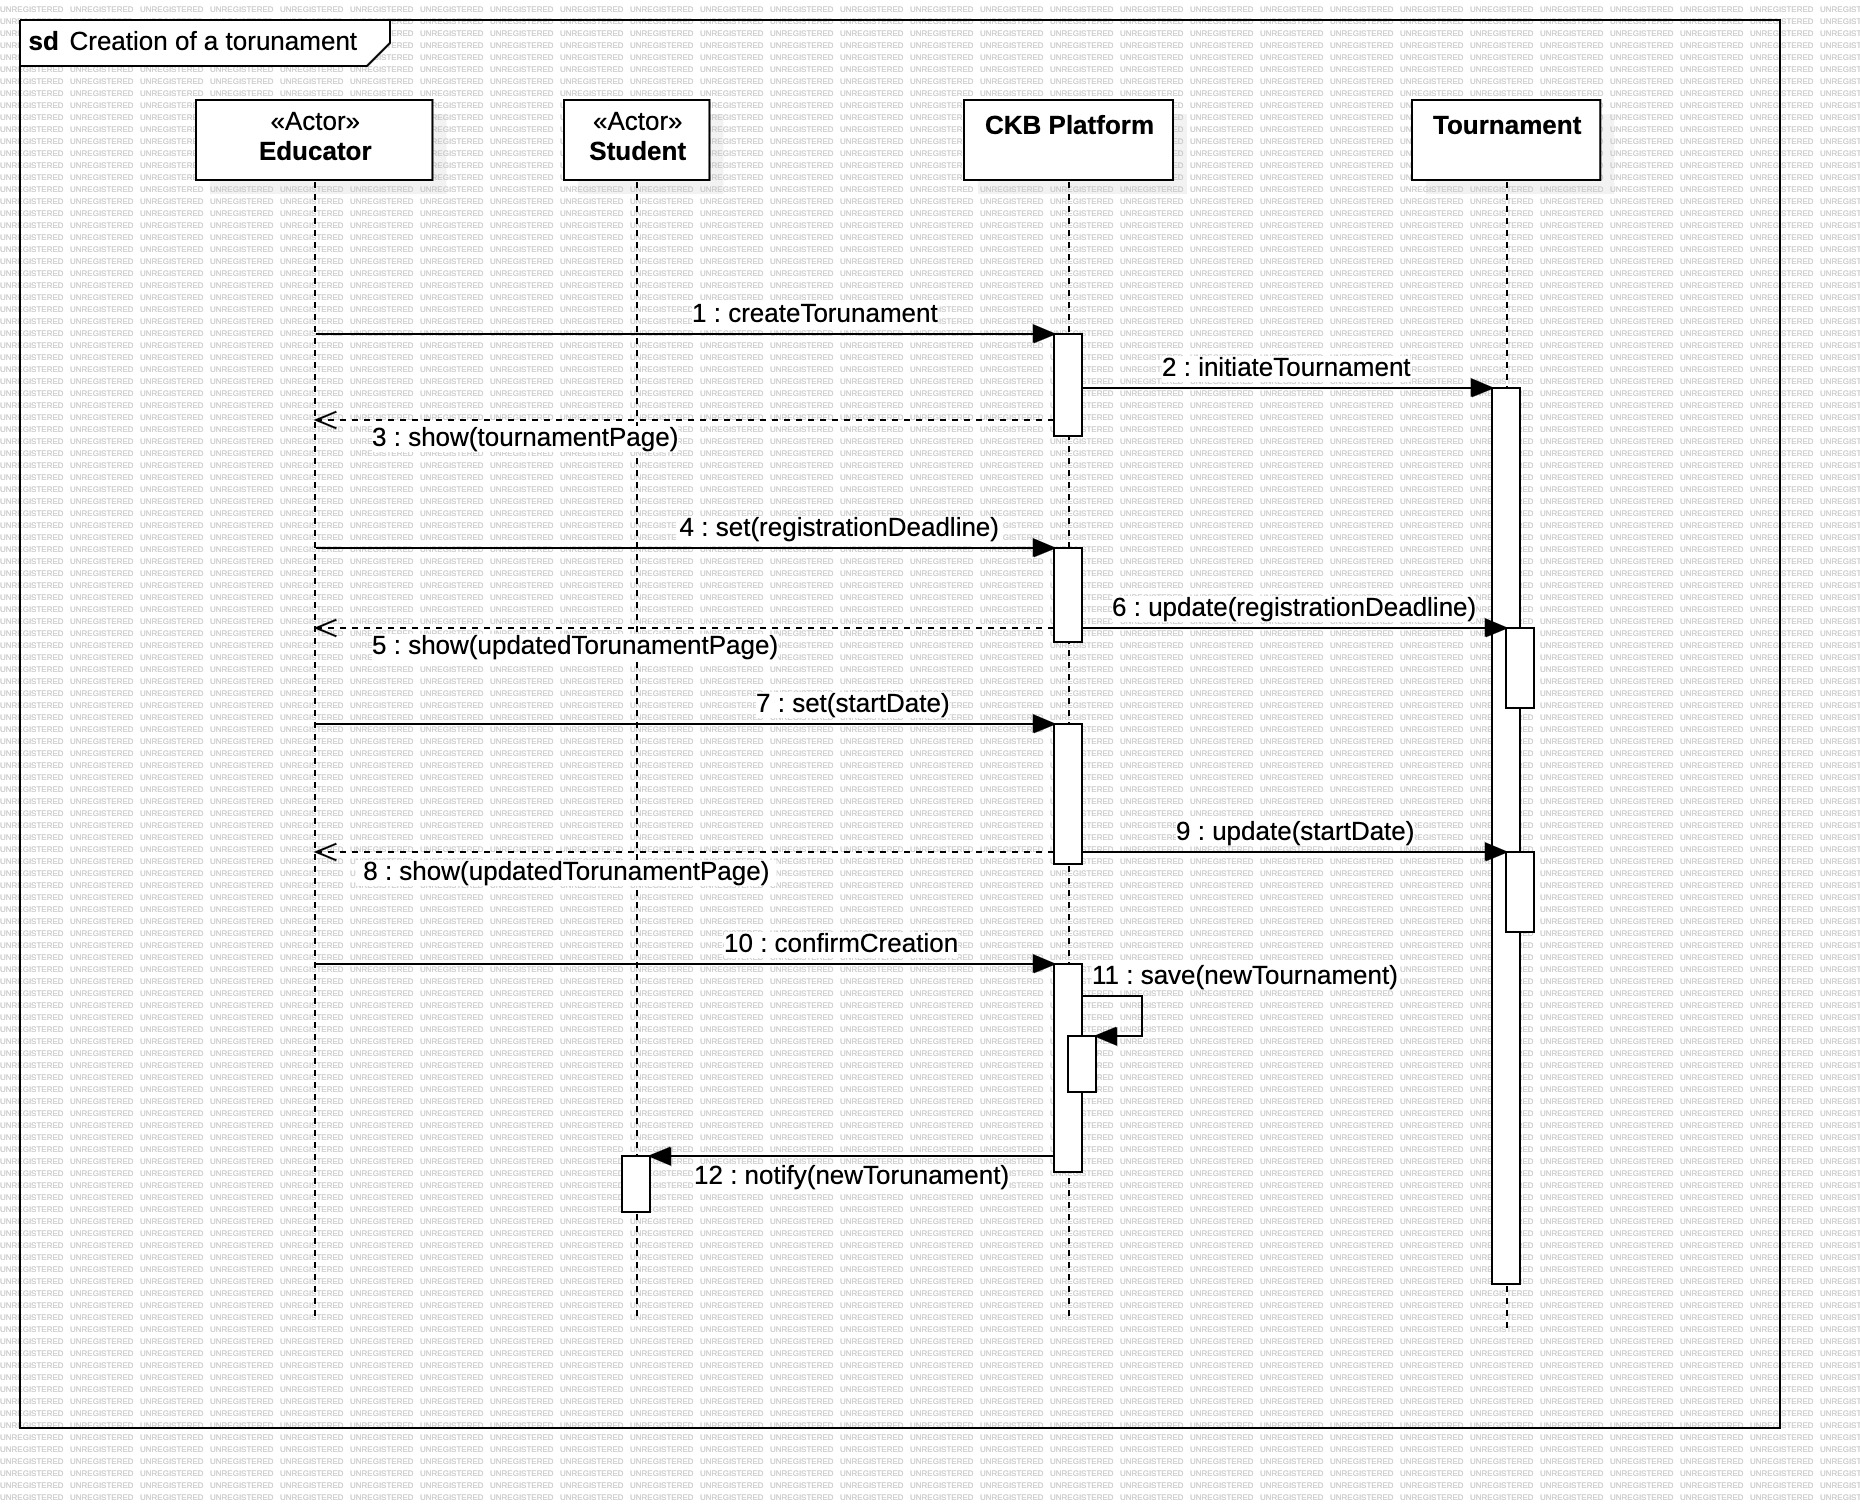
\includegraphics[width=\textwidth]{Diagrams/TournamentCreationSD.jpg}
    \caption{Sequence Diagram - Creation of a tournament}
    \label{fig:sequence-diagram-create-tournament}
\end{figure}

\subsubsection*{[UC3] Close a tournament}
\begin{figure}[H]
    \centering
    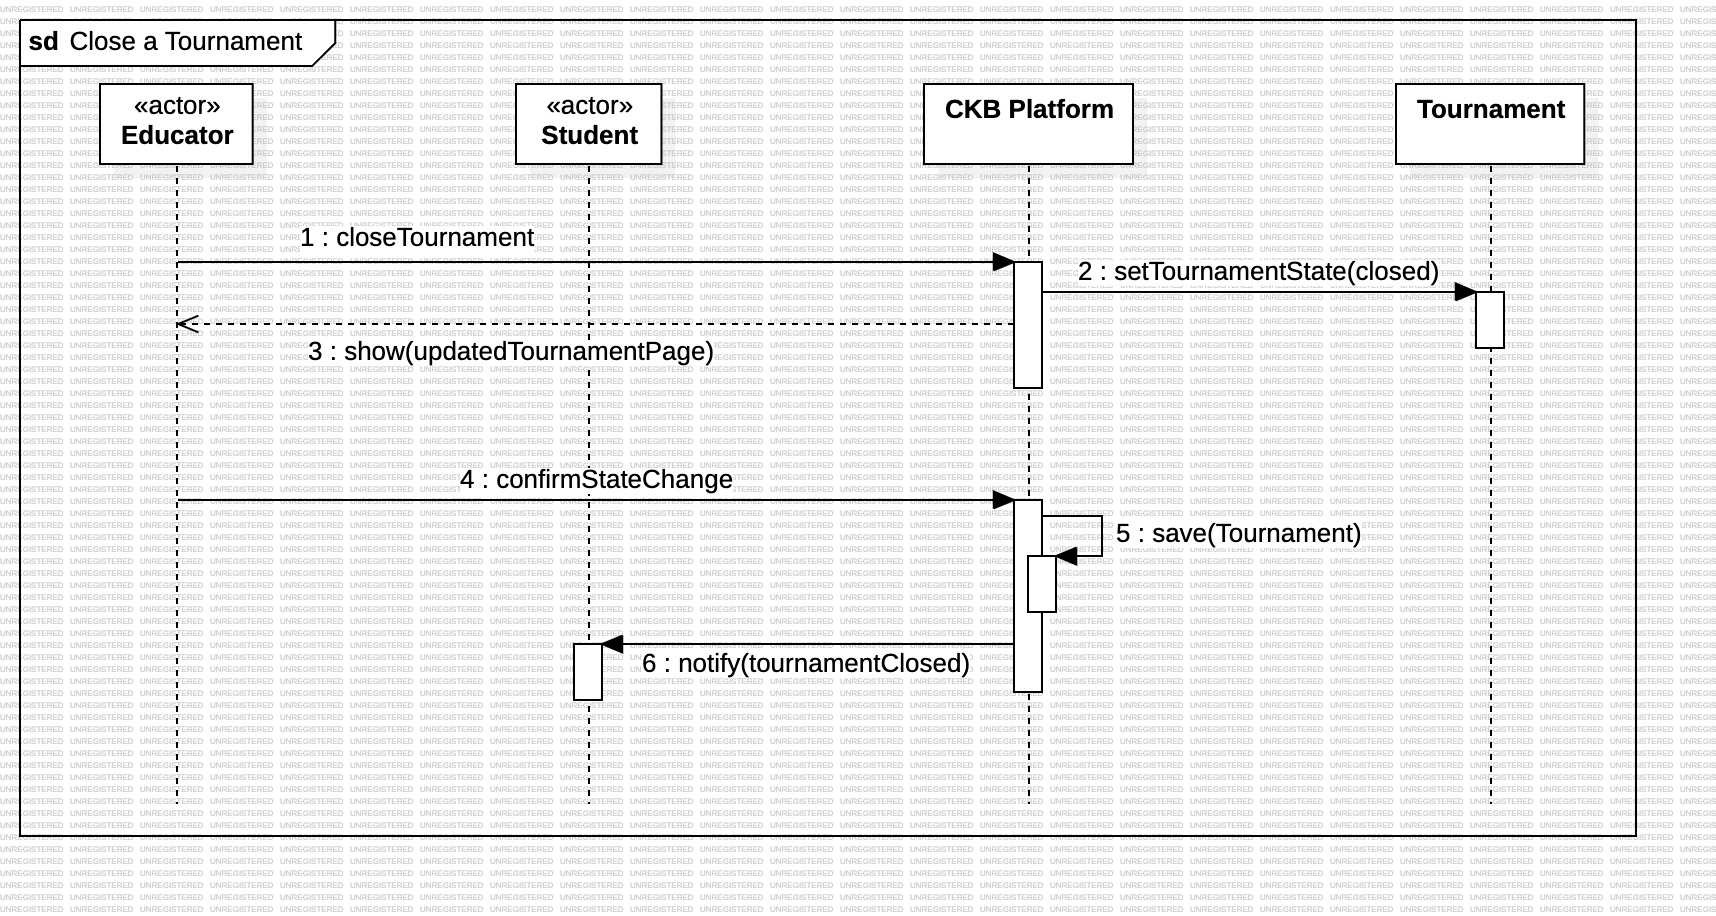
\includegraphics[width=\textwidth]{Diagrams/UC3SequenceDiagram.jpg}
    \caption{Sequence Diagram for the Close a tournament Use Case}
    \label{fig:sequence-diagram-close-tournament}
\end{figure}

\subsubsection*{[UC4] Creation of a battle}
\begin{figure}[H]
    \centering
    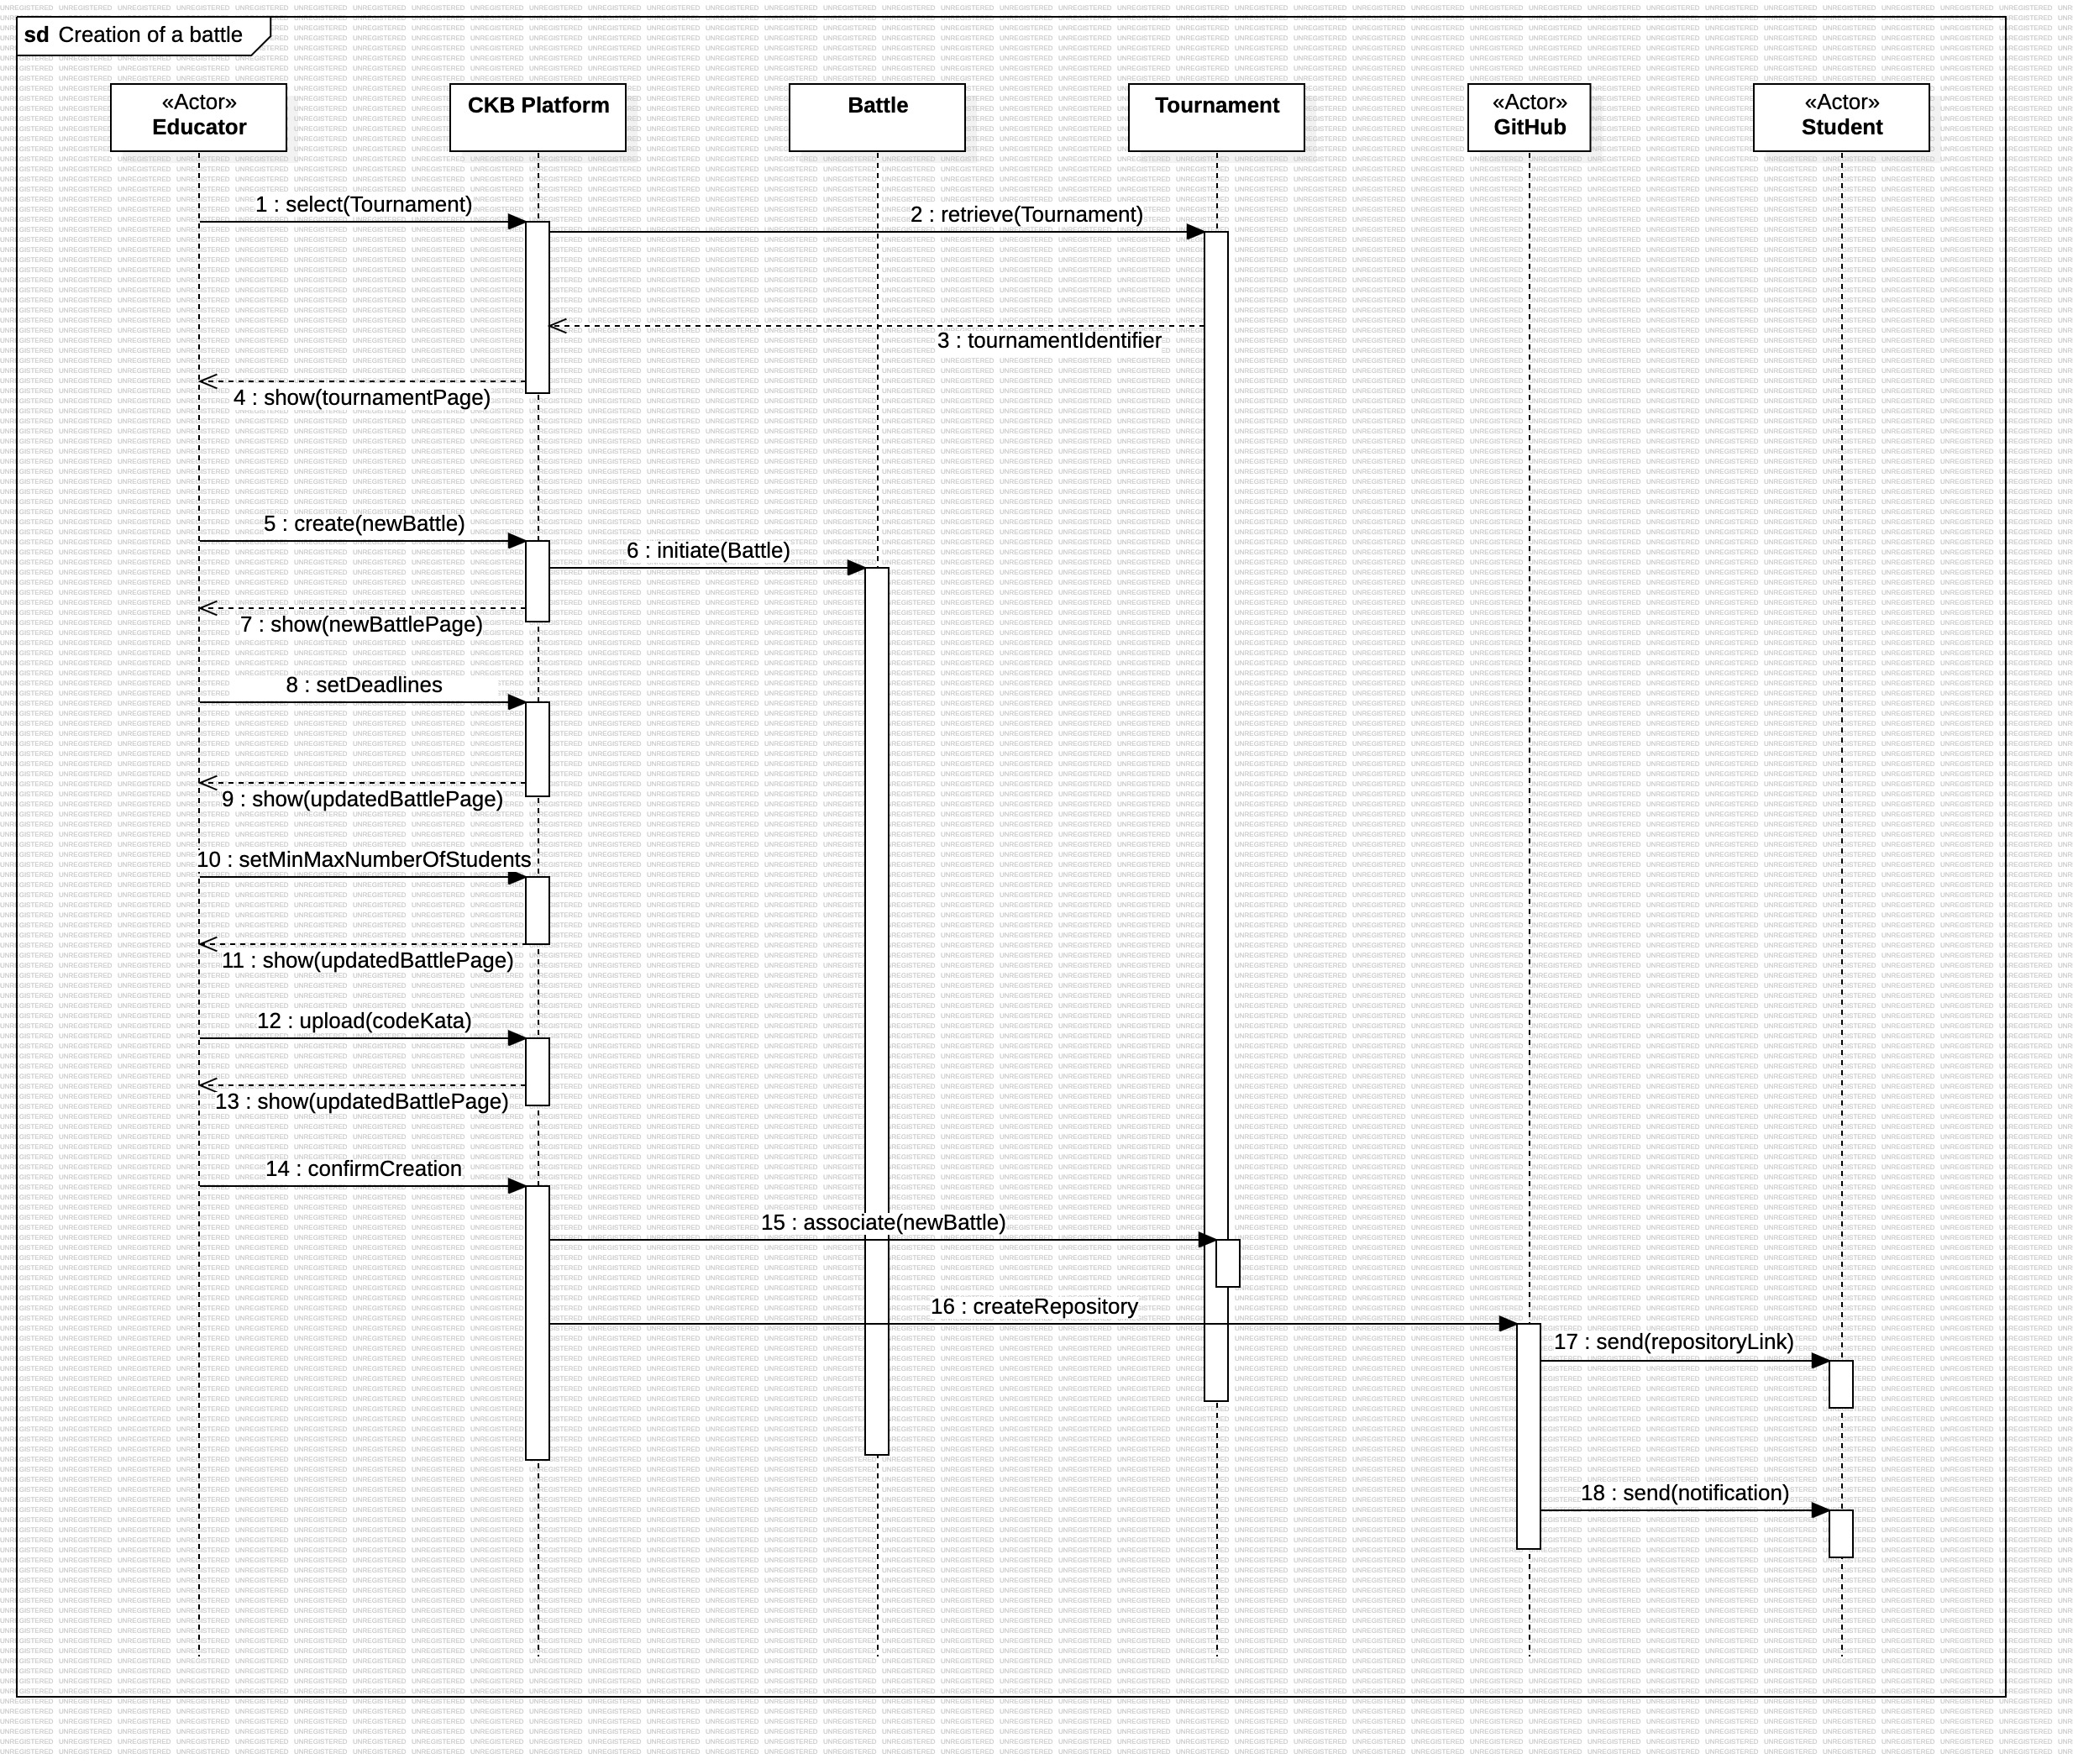
\includegraphics[width=\textwidth]{Diagrams/BattleCreation.jpg}
    \caption{Sequence Diagram - Creation of a battle}
    \label{fig:sequence-diagram-create-battle}
\end{figure}

\subsubsection*{[UC5] Upload of code kata}
\begin{figure}[H]
    \centering
    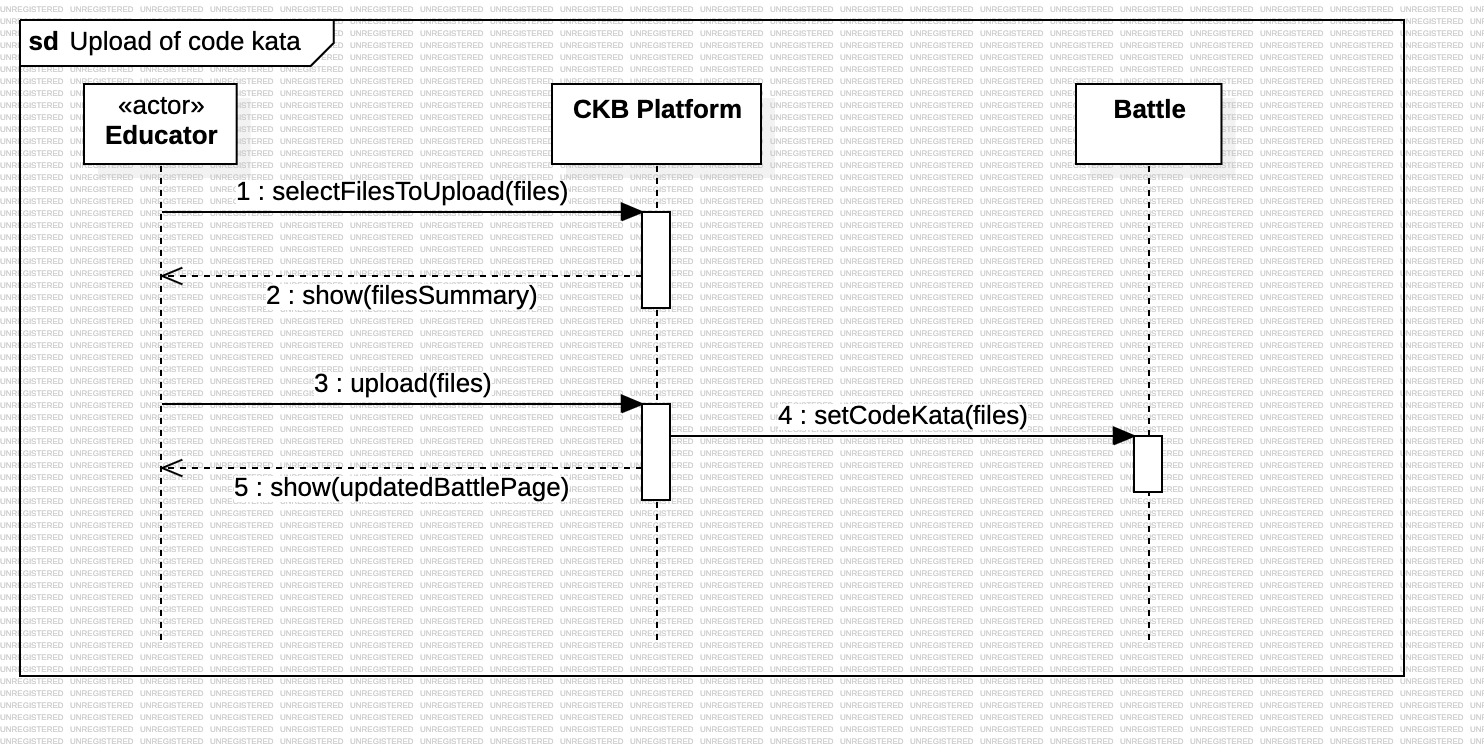
\includegraphics[width=\textwidth]{Diagrams/UC5SequenceDiagram.jpg}
    \caption{Sequence Diagram for the Upload of code kata Use Case}
    \label{fig:sequence-diagram-upload-code-kata}
\end{figure}

\subsubsection*{[UC6] Manual score update}
\begin{figure}[H]
    \centering
    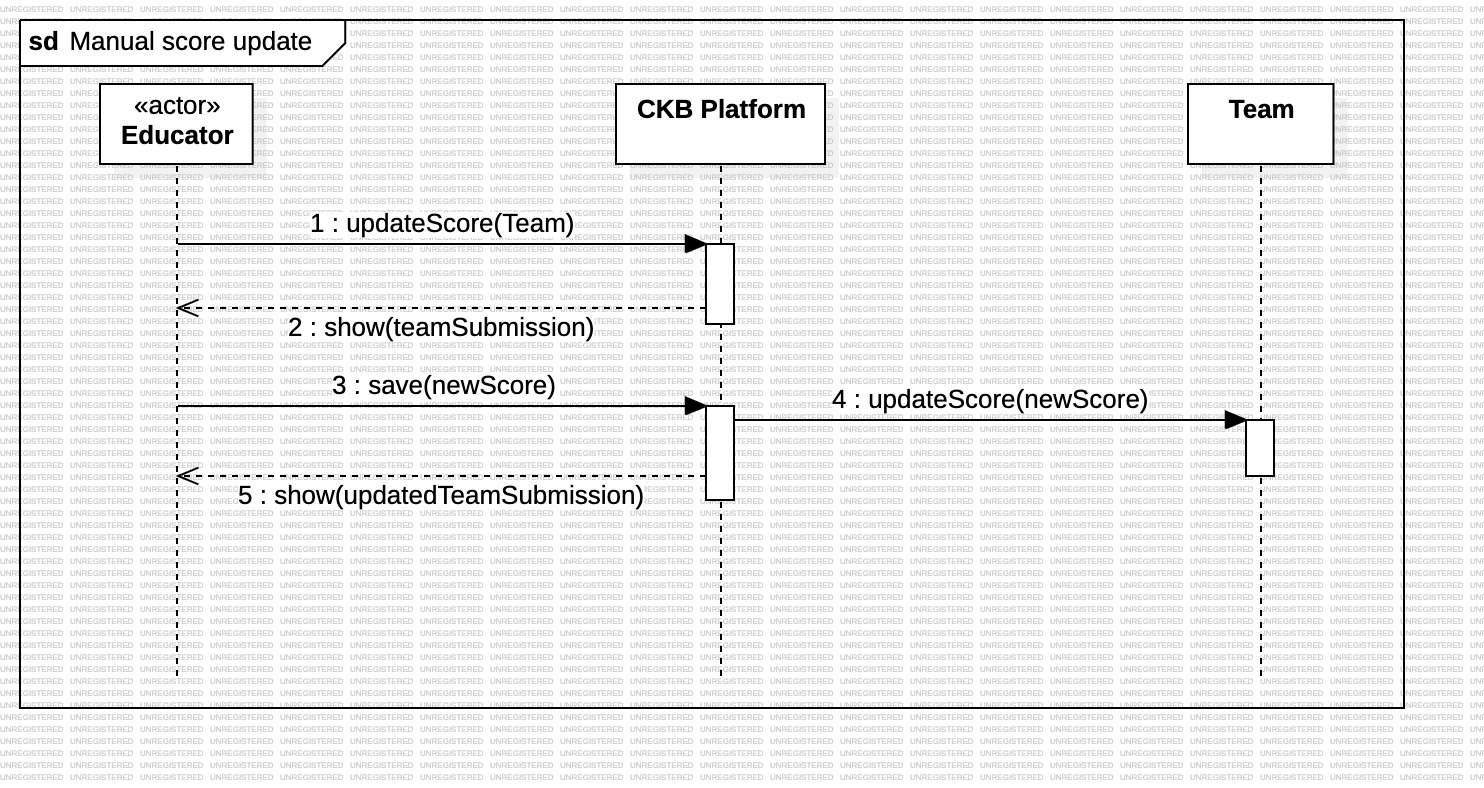
\includegraphics[width=\textwidth]{Diagrams/UC6SequenceDiagram.jpg}
    \caption{Sequence Diagram for the Manual score update Use Case}
    \label{fig:sequence-diagram-manual-score-update}
\end{figure}

\subsubsection*{[UC7] Invite othe educators to a tournament}
\begin{figure}[H]
    \centering
    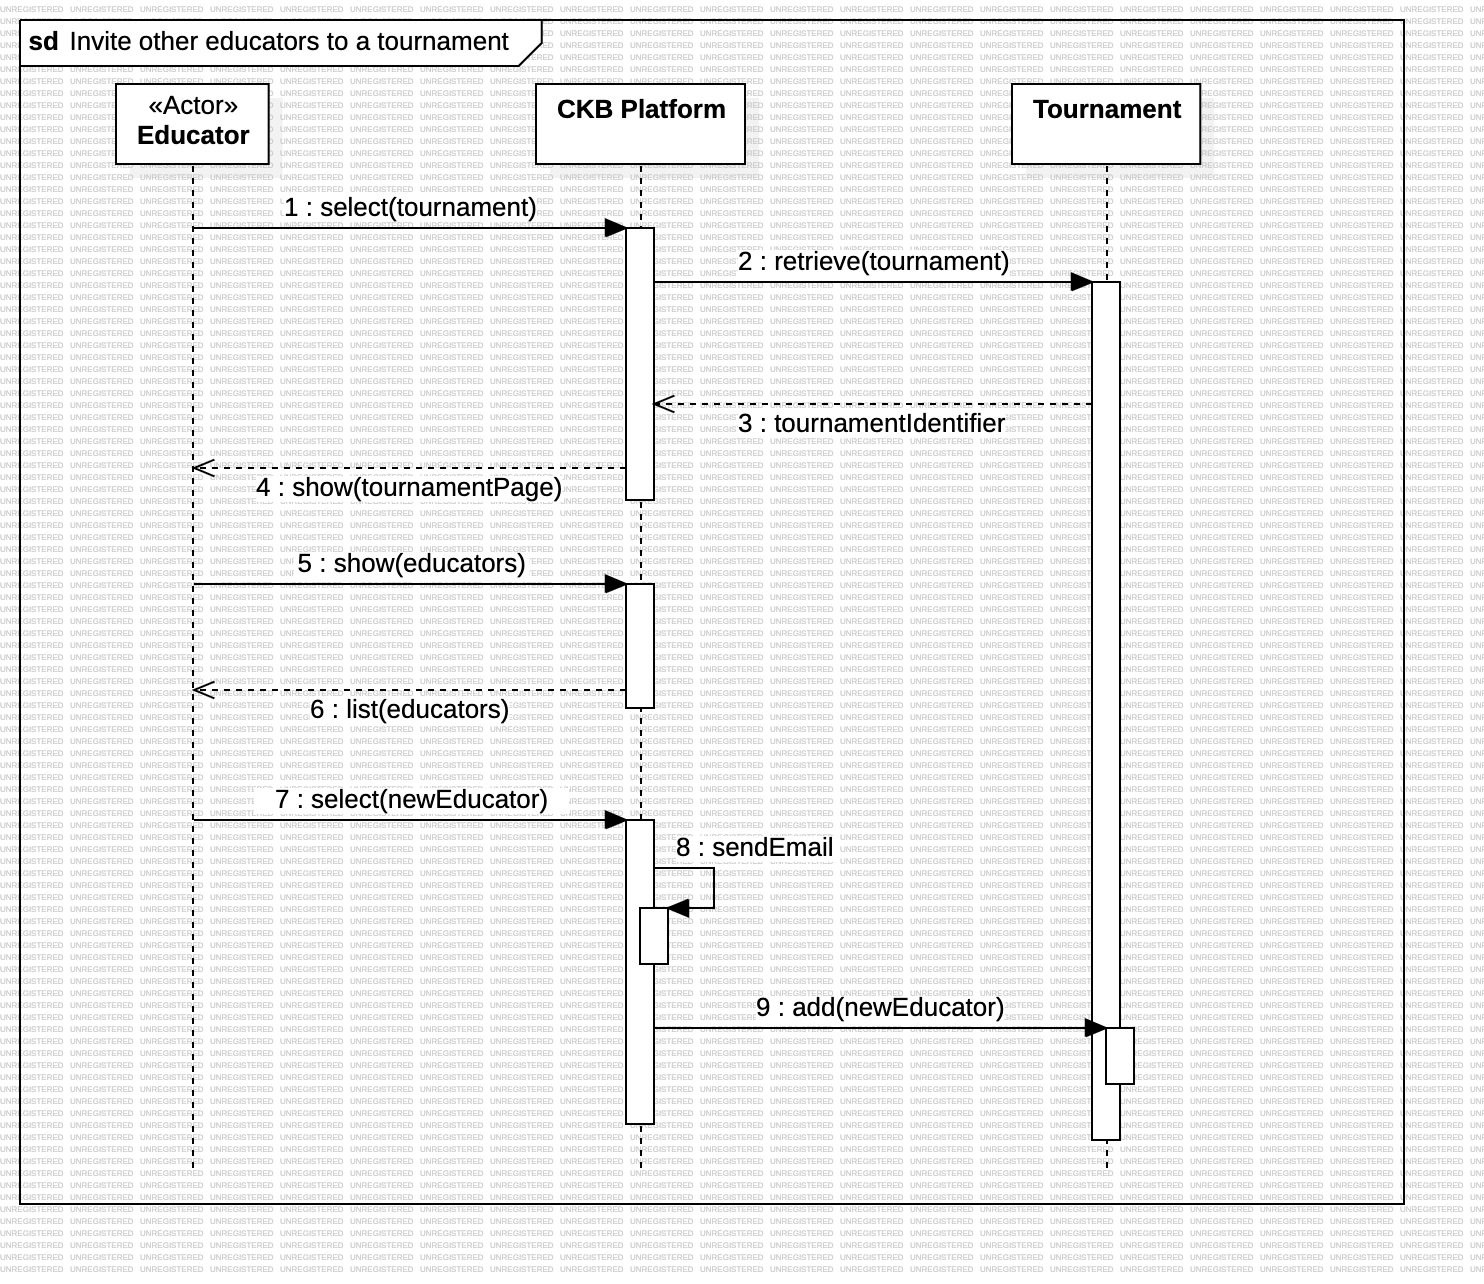
\includegraphics[width=\textwidth]{Diagrams/InviteEducators.jpg}
    \caption{Sequence Diagram - Invite other educators to a tournament}
    \label{fig:sequence-diagram-invite-educator}
\end{figure}
\subsubsection*{[UC8] Notification to a student}
\begin{figure}[H]
    \centering
    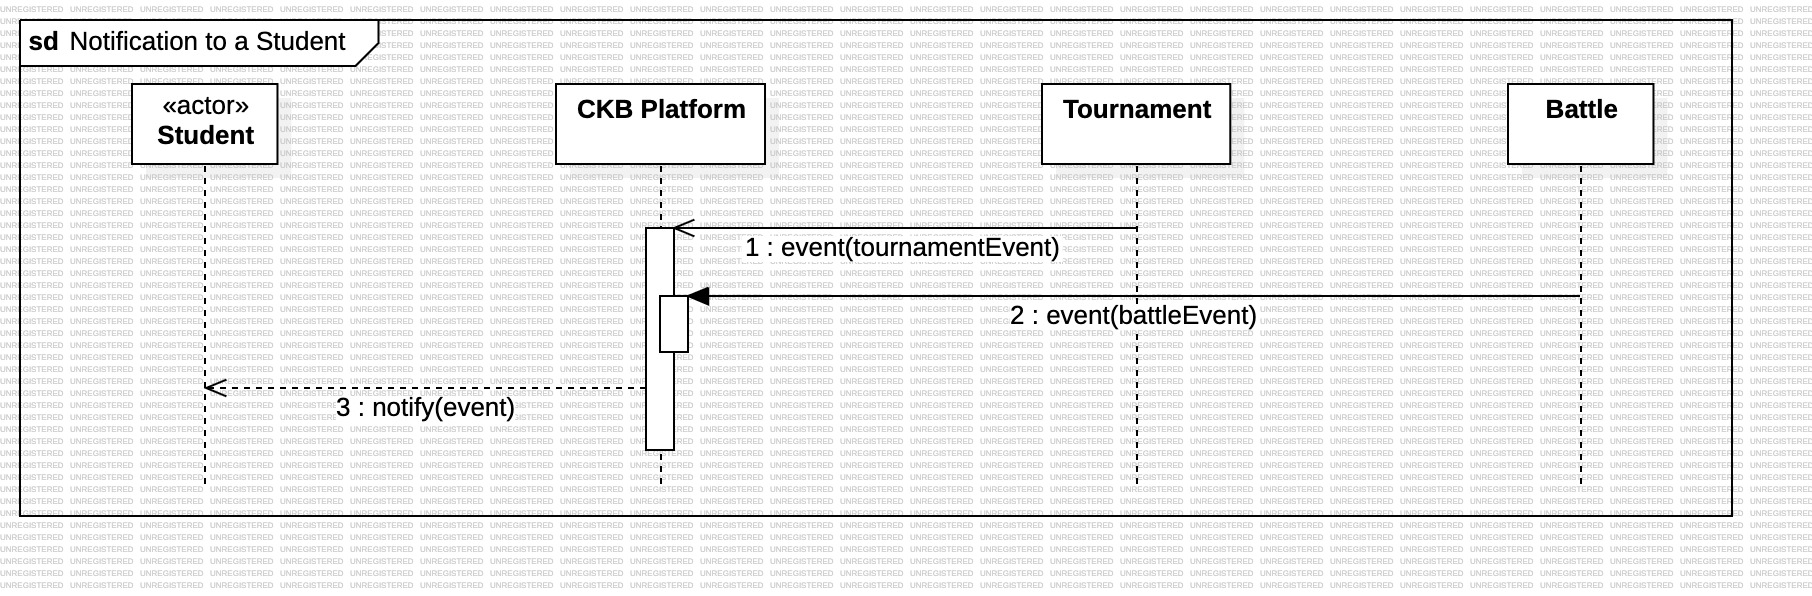
\includegraphics[width=\textwidth]{Diagrams/UC8SequenceDiagram.jpg}
    \caption{Sequence Diagram for the Notification to a student Use Case}
    \label{fig:sequence-diagram-notification}
\end{figure}

\subsubsection*{[UC9] Subscribe to a tournament}
\begin{figure}[H]
    \centering
    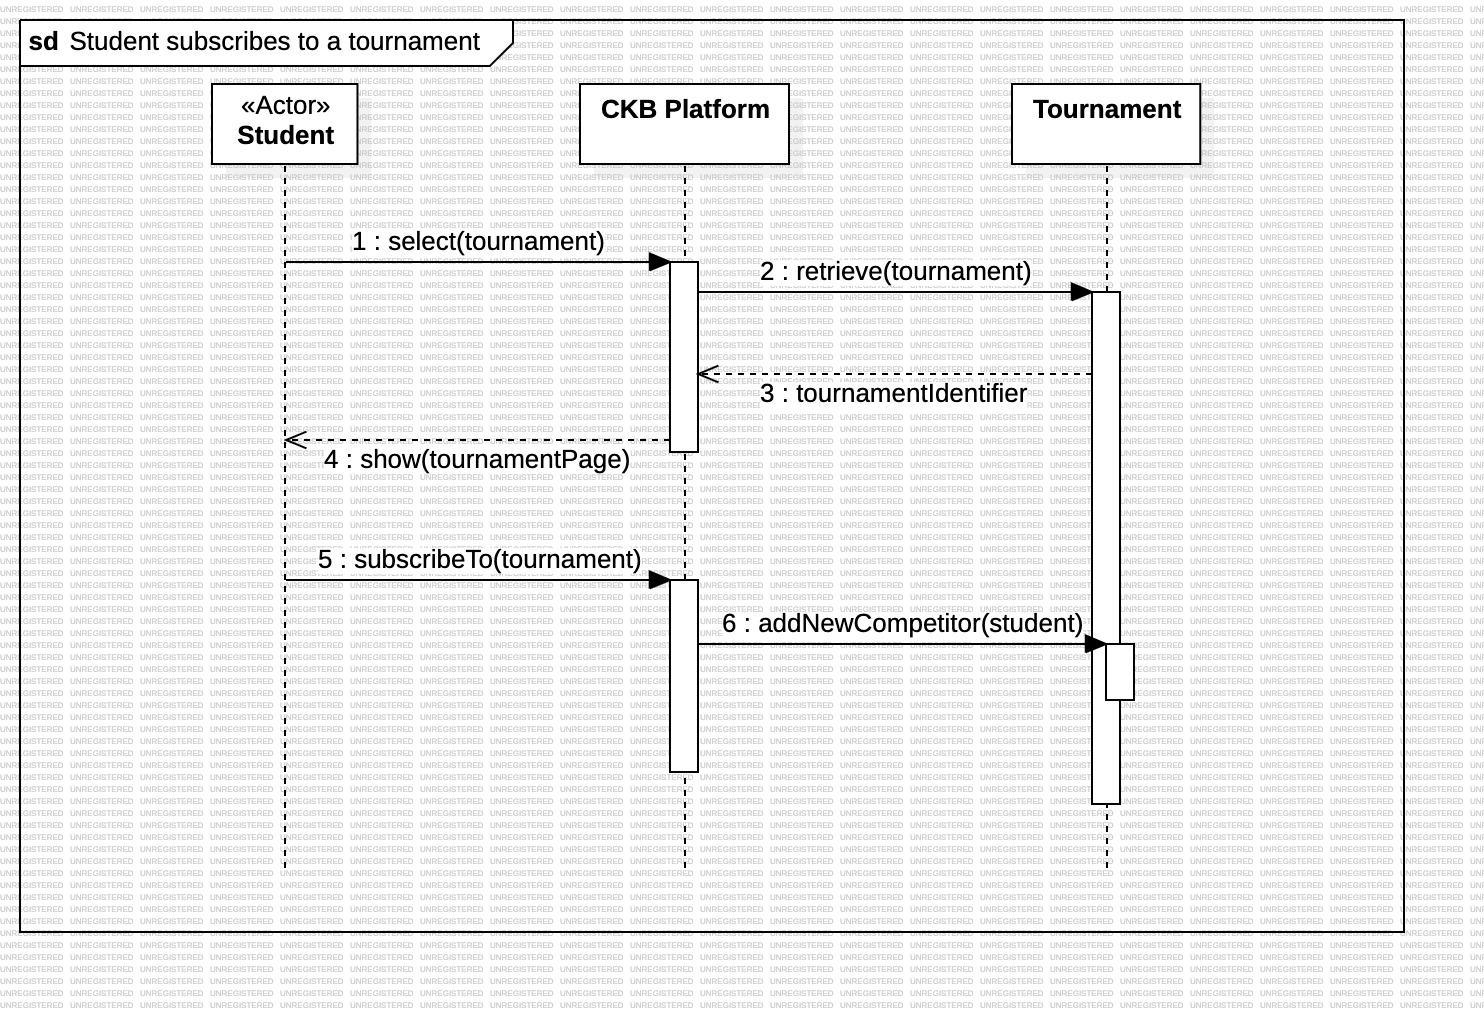
\includegraphics[width=\textwidth]{Diagrams/StudentSubscription.jpg}
    \caption{Sequence Diagram - Subscribe to a tournament}
    \label{fig:sequence-diagram-subscribe-tournament}
\end{figure}
\subsubsection*{[UC10] Subscribe to a battle}
\begin{figure}[H]
    \centering
    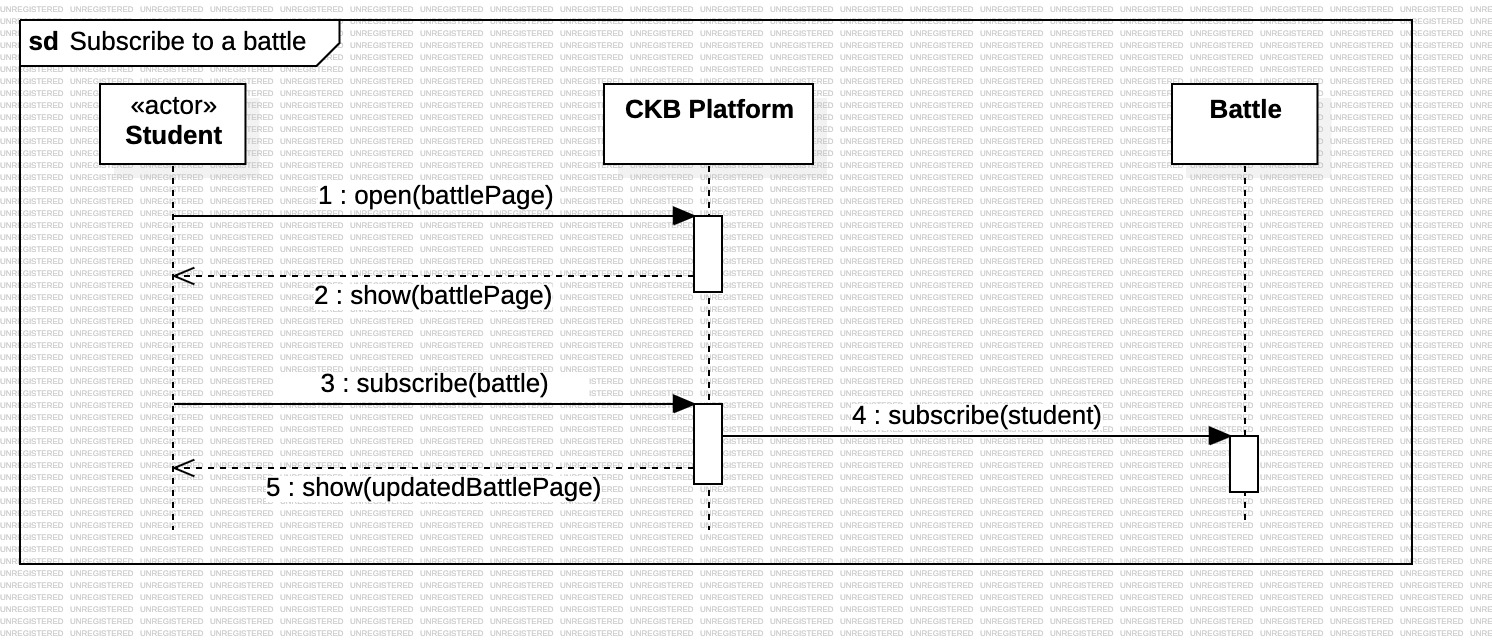
\includegraphics[width=\textwidth]{Diagrams/UC10SequenceDiagram.jpg}
    \caption{Sequence Diagram for the Subscribe to a battle Use Case}
    \label{fig:sequence-diagram-subscribe-battle}
\end{figure}

\subsubsection*{[UC11] Accept invitation to a team for a battle}
\begin{figure}[H]
    \centering
    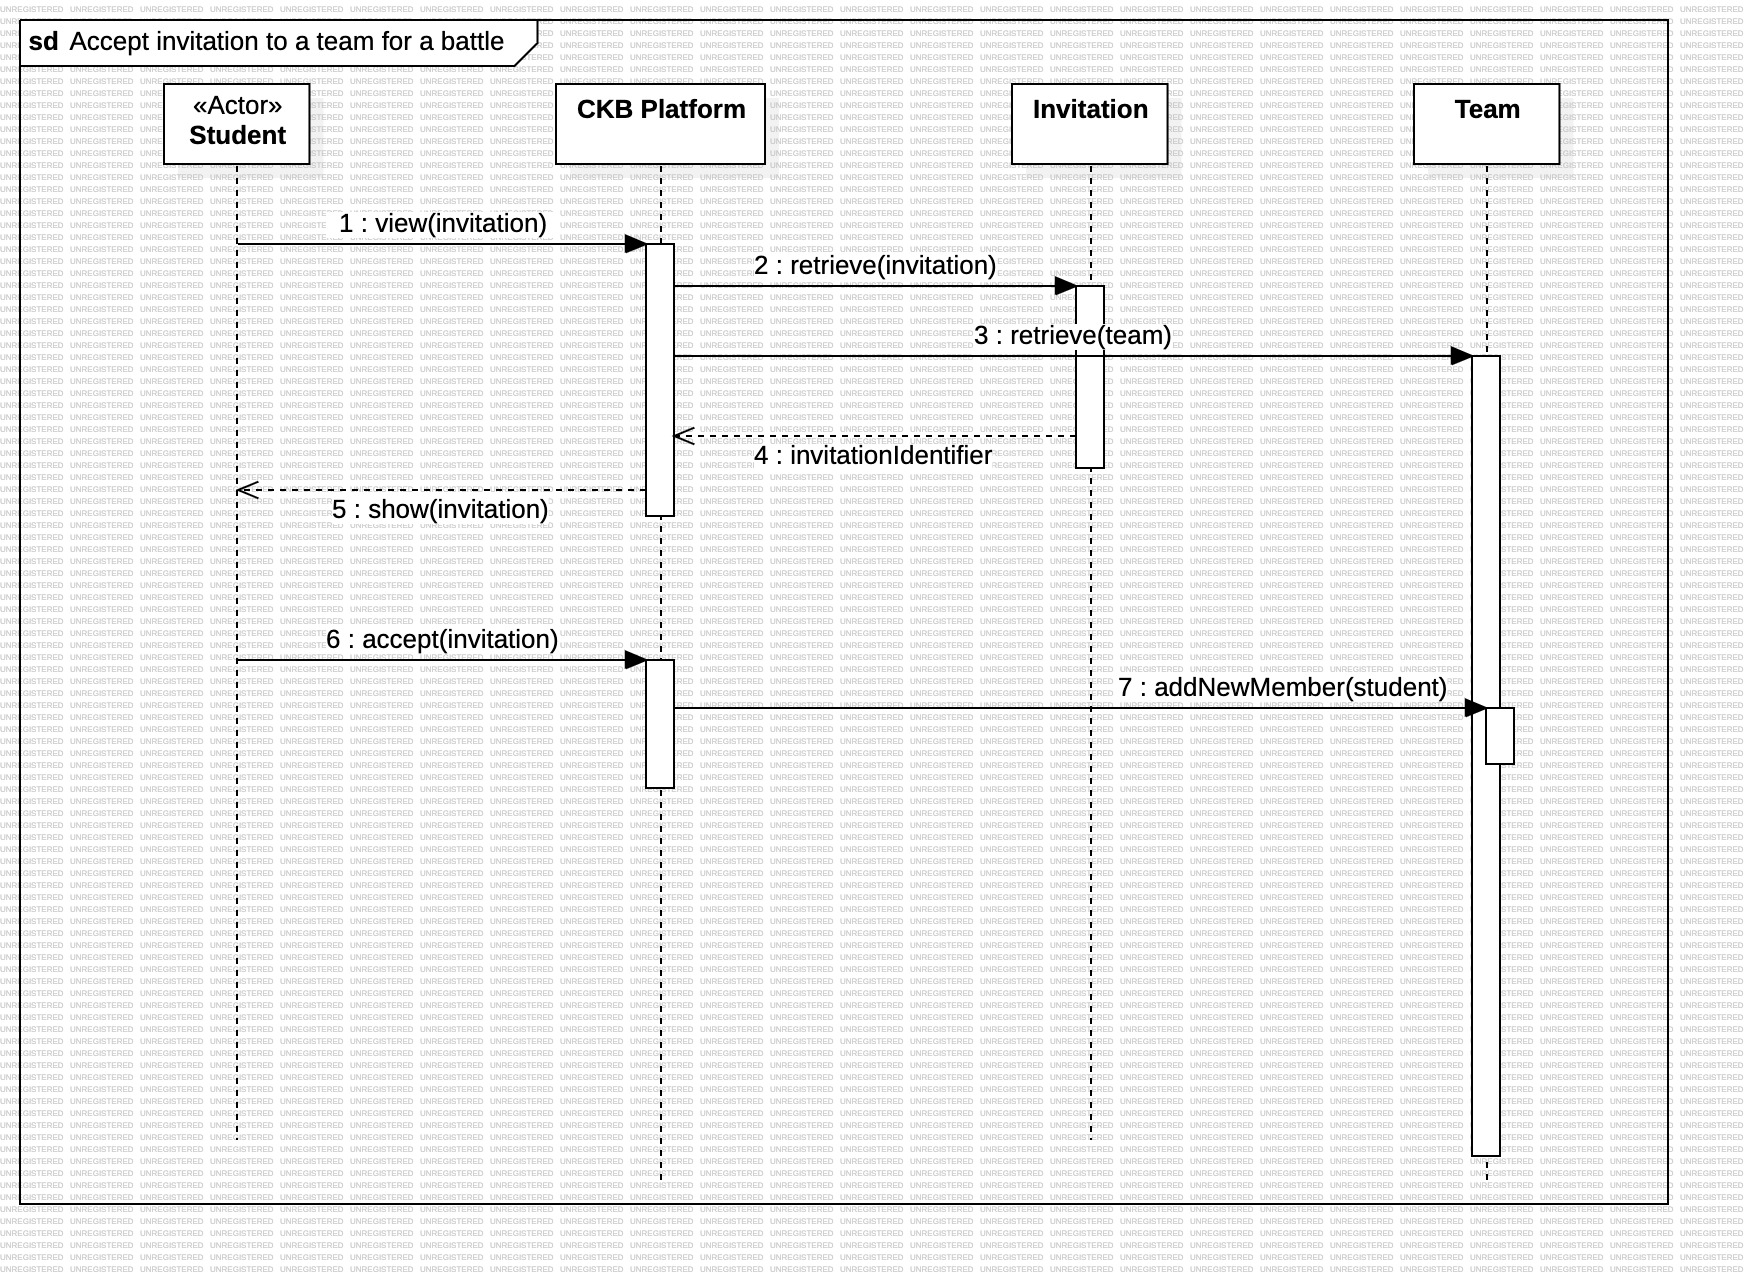
\includegraphics[width=\textwidth]{Diagrams/StudentAcceptInvitation.jpg}
    \caption{Sequence Diagram - Accept invitation to a team for a battle}
    \label{fig:sequence-diagram-accept-invitation}
\end{figure}

\subsubsection*{[UC12] Creation of a team for a battle}
\begin{figure}[H]
    \centering
    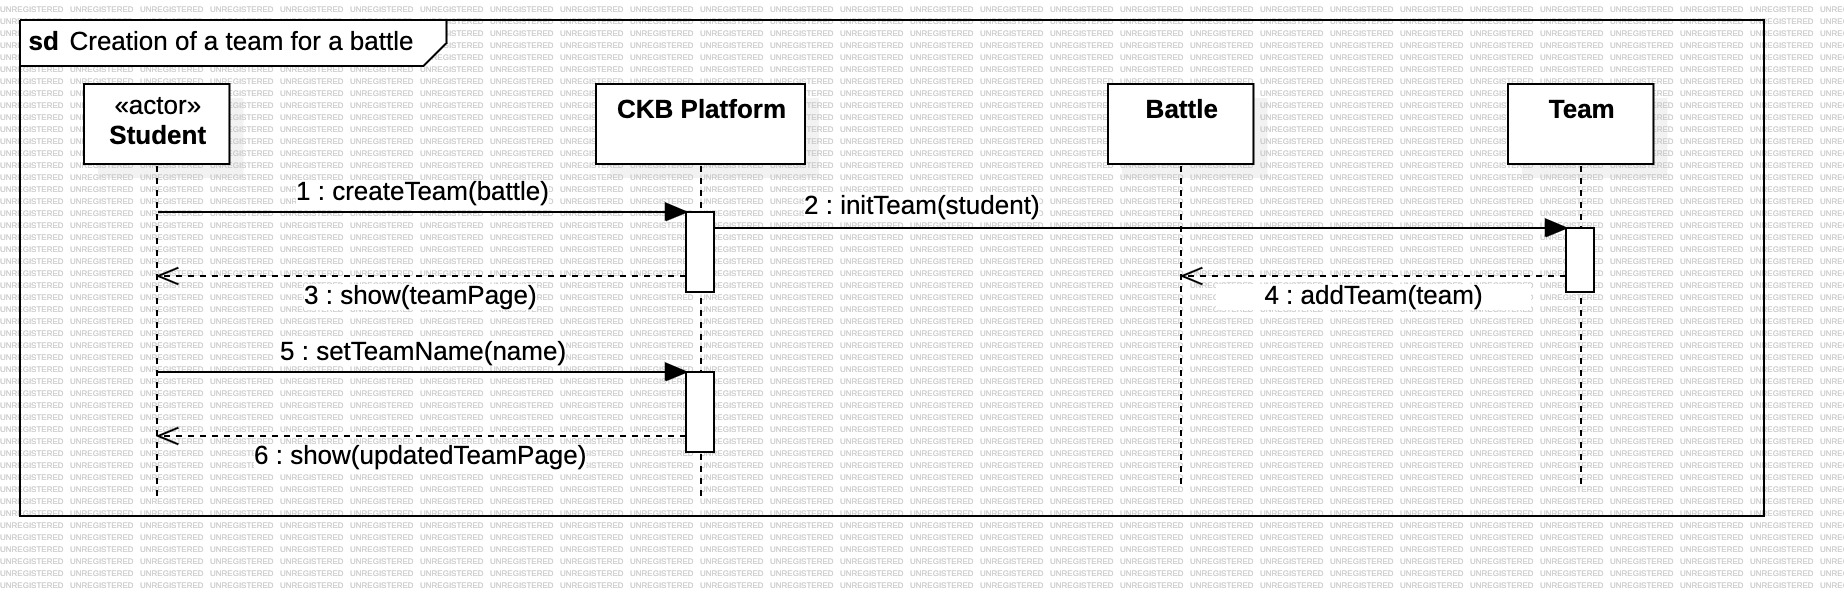
\includegraphics[width=\textwidth]{Diagrams/UC12SequenceDiagram.jpg}
    \caption{Sequence Diagram for the Creation of a team for a battle Use Case}
    \label{fig:sequence-diagram-create-team}
\end{figure}

\subsubsection*{[UC13] Invite other students to the team}
\begin{figure}[H]
    \centering
    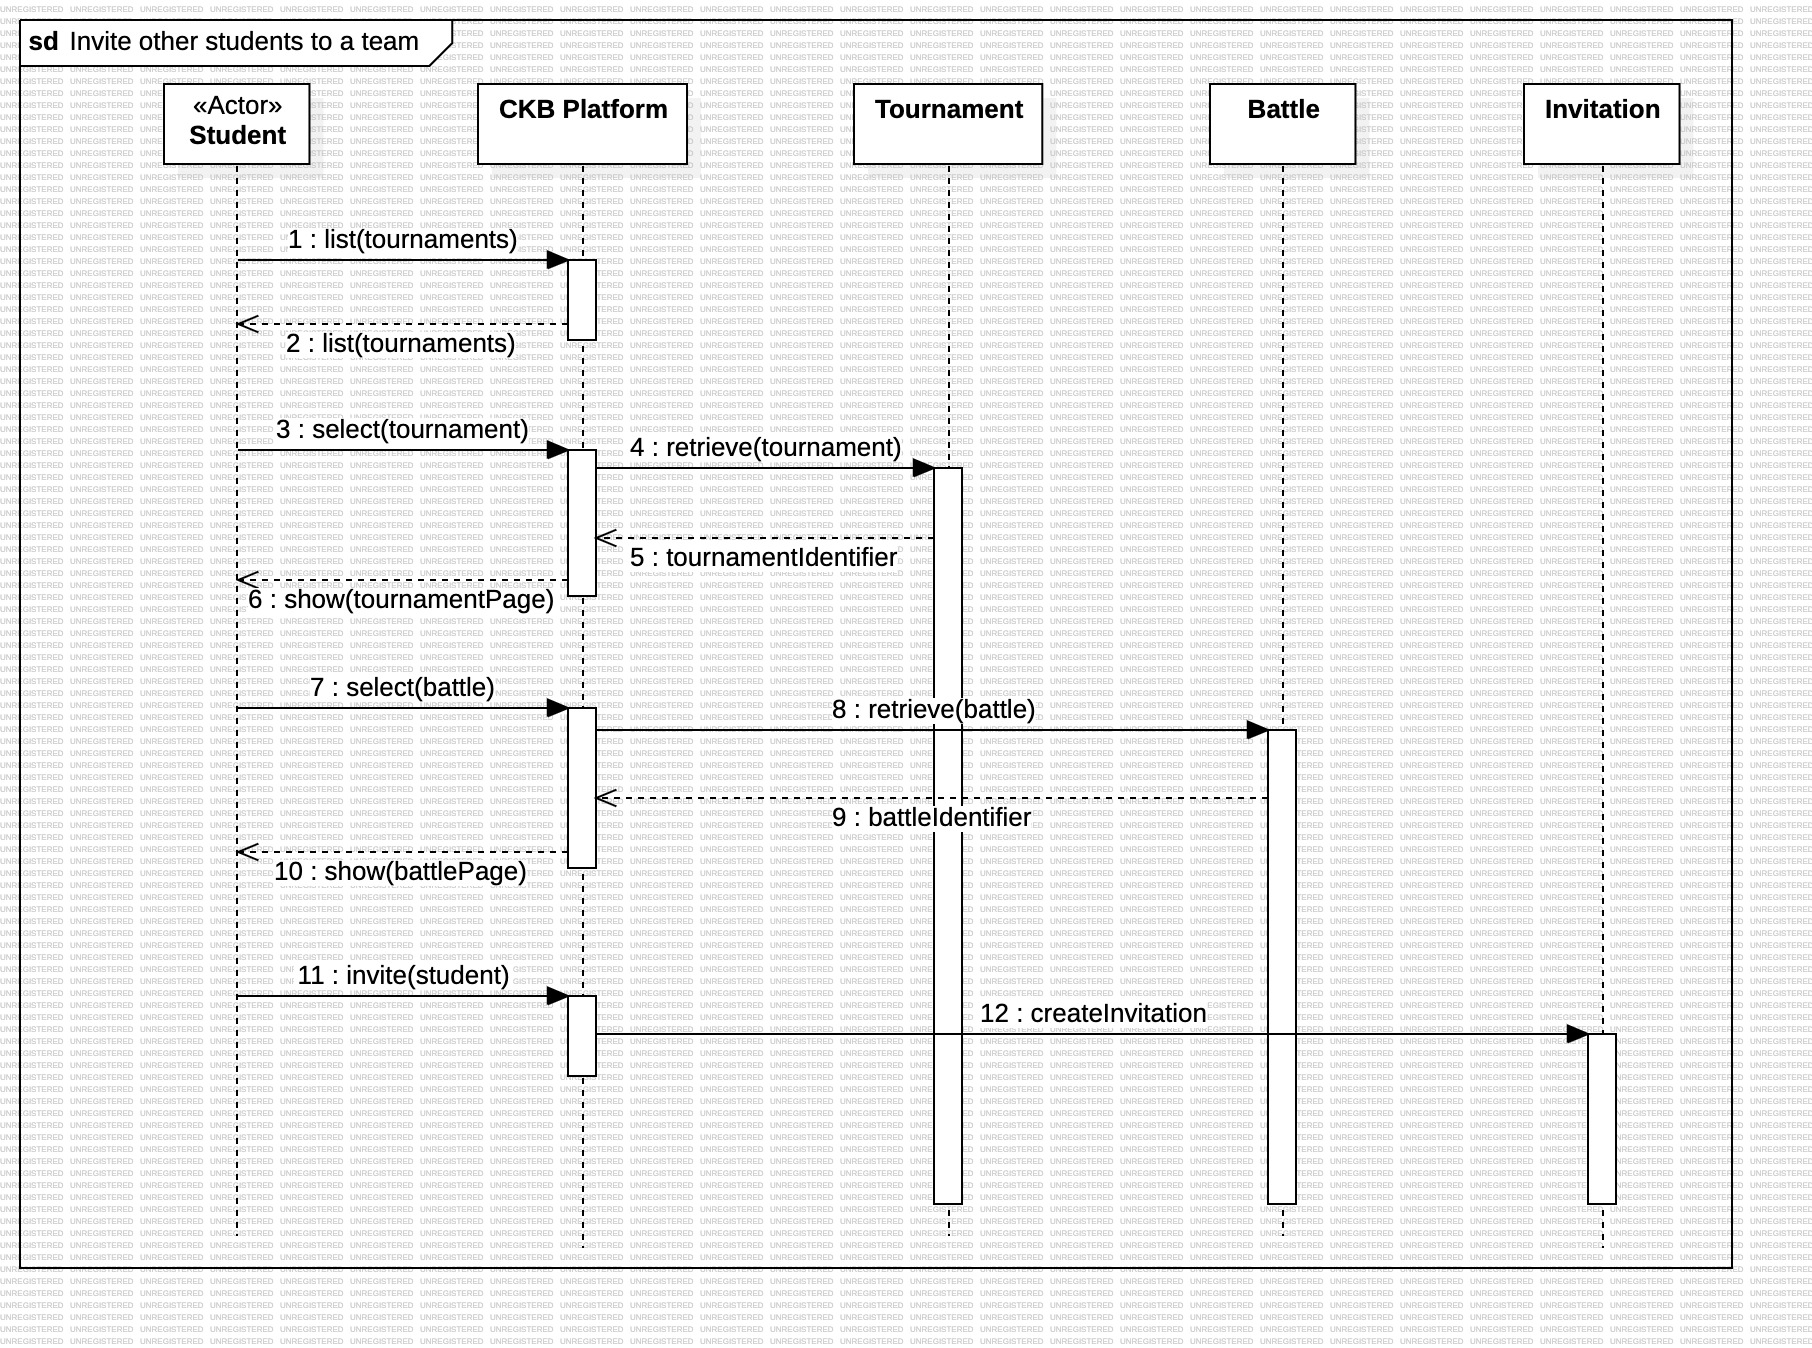
\includegraphics[width=\textwidth]{Diagrams/StudentInvitation.jpg}
    \caption{Sequence Diagram - Invite other students to the team}
    \label{fig:sequence-diagram-invite-students}
\end{figure}

\subsubsection*{[UC14] Fork repository of a battle}
\begin{figure}[H]
    \centering
    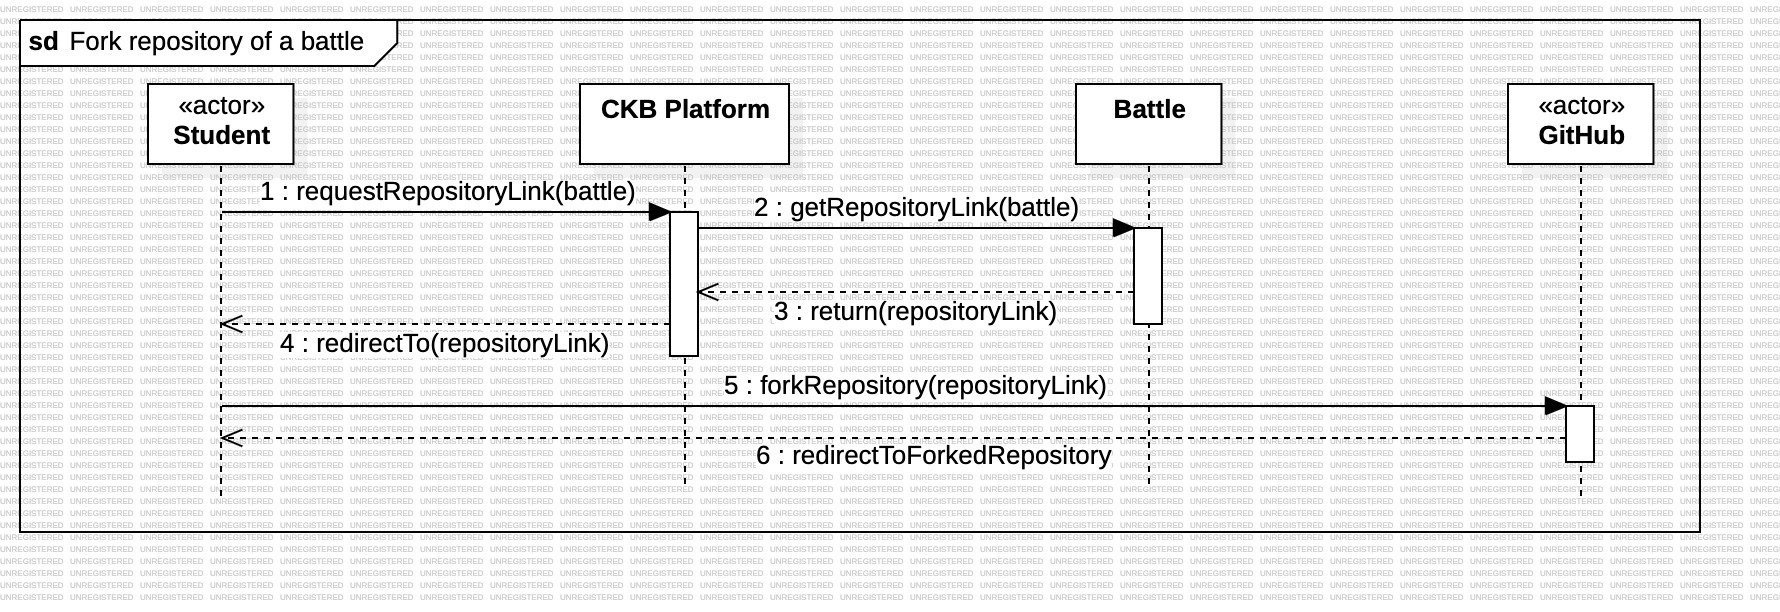
\includegraphics[width=\textwidth]{Diagrams/UC14SequenceDiagram.jpg}
    \caption{Sequence Diagram for the Fork repository of a battle Use Case}
    \label{fig:sequence-diagram-fork-repository}
\end{figure}

\subsubsection*{[UC15] Submission of a solution for a battle}
\begin{figure}[H]
    \centering
    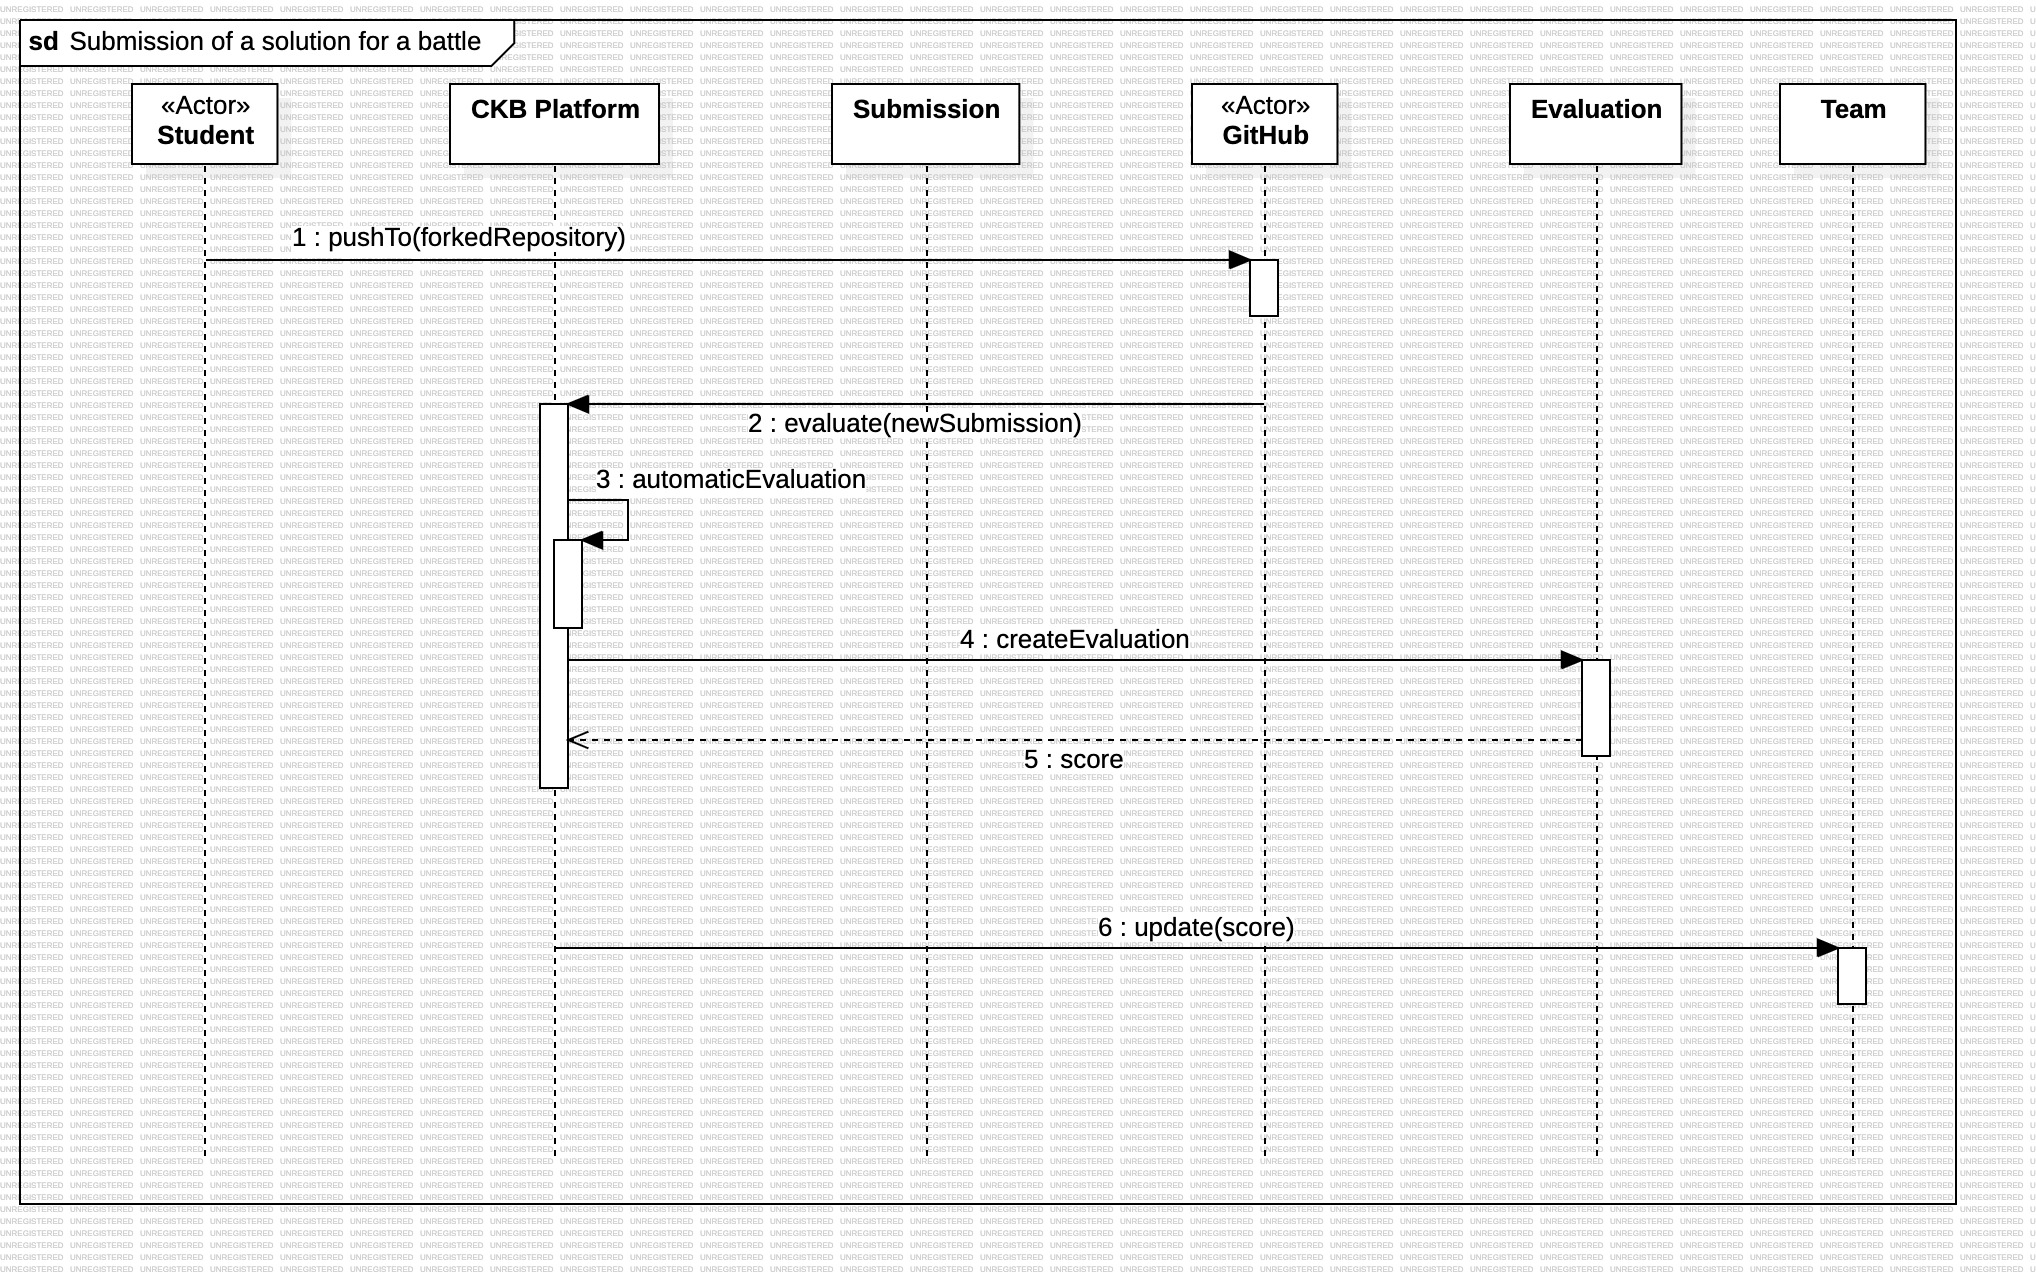
\includegraphics[width=\textwidth]{Diagrams/Submission.jpg}
    \caption{Sequence Diagram - Submission of a solution for a battle}
    \label{fig:sequence-diagram-submission}
\end{figure}

\subsubsection*{[UC16] Push on team repository}
\begin{figure}[H]
    \centering
    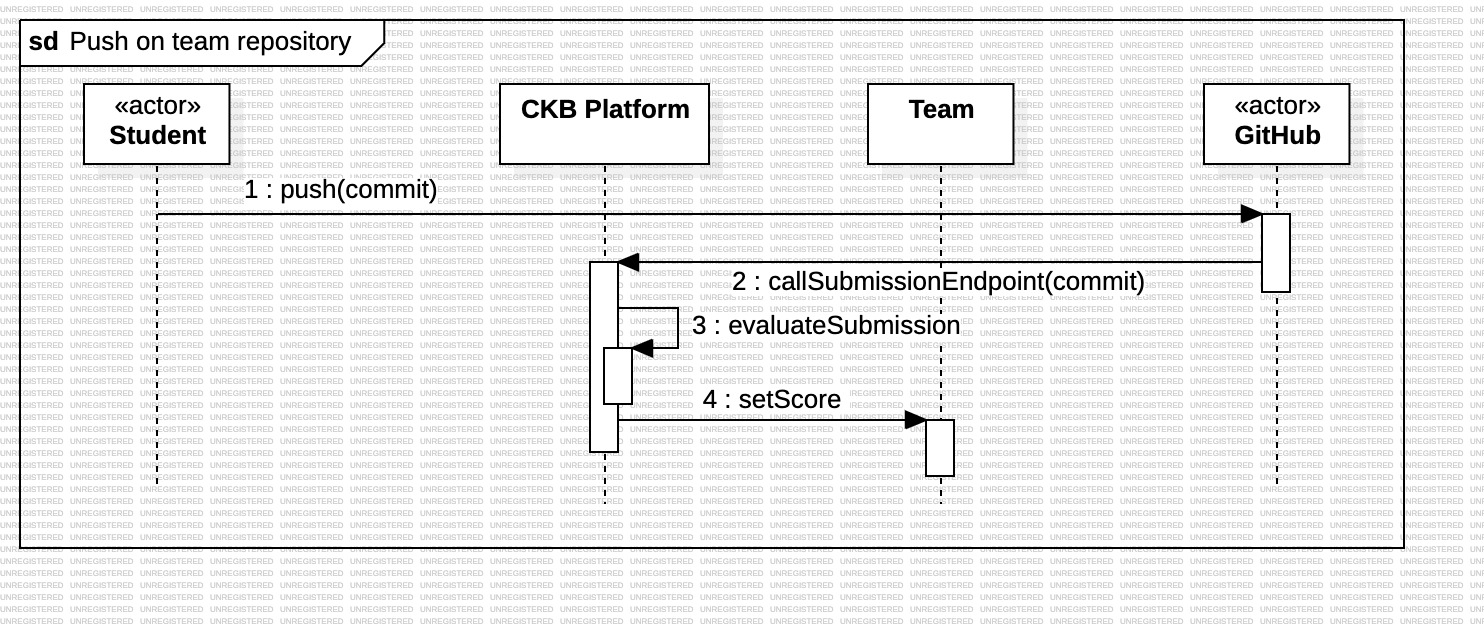
\includegraphics[width=\textwidth]{Diagrams/UC16SequenceDiagram.jpg}
    \caption{Sequence Diagram for the Push on team repository Use Case}
    \label{fig:sequence-diagram-push-repository}
\end{figure}

\subsubsection*{[UC17] Automatic evaluation of a submission}
\begin{figure}[H]
    \centering
    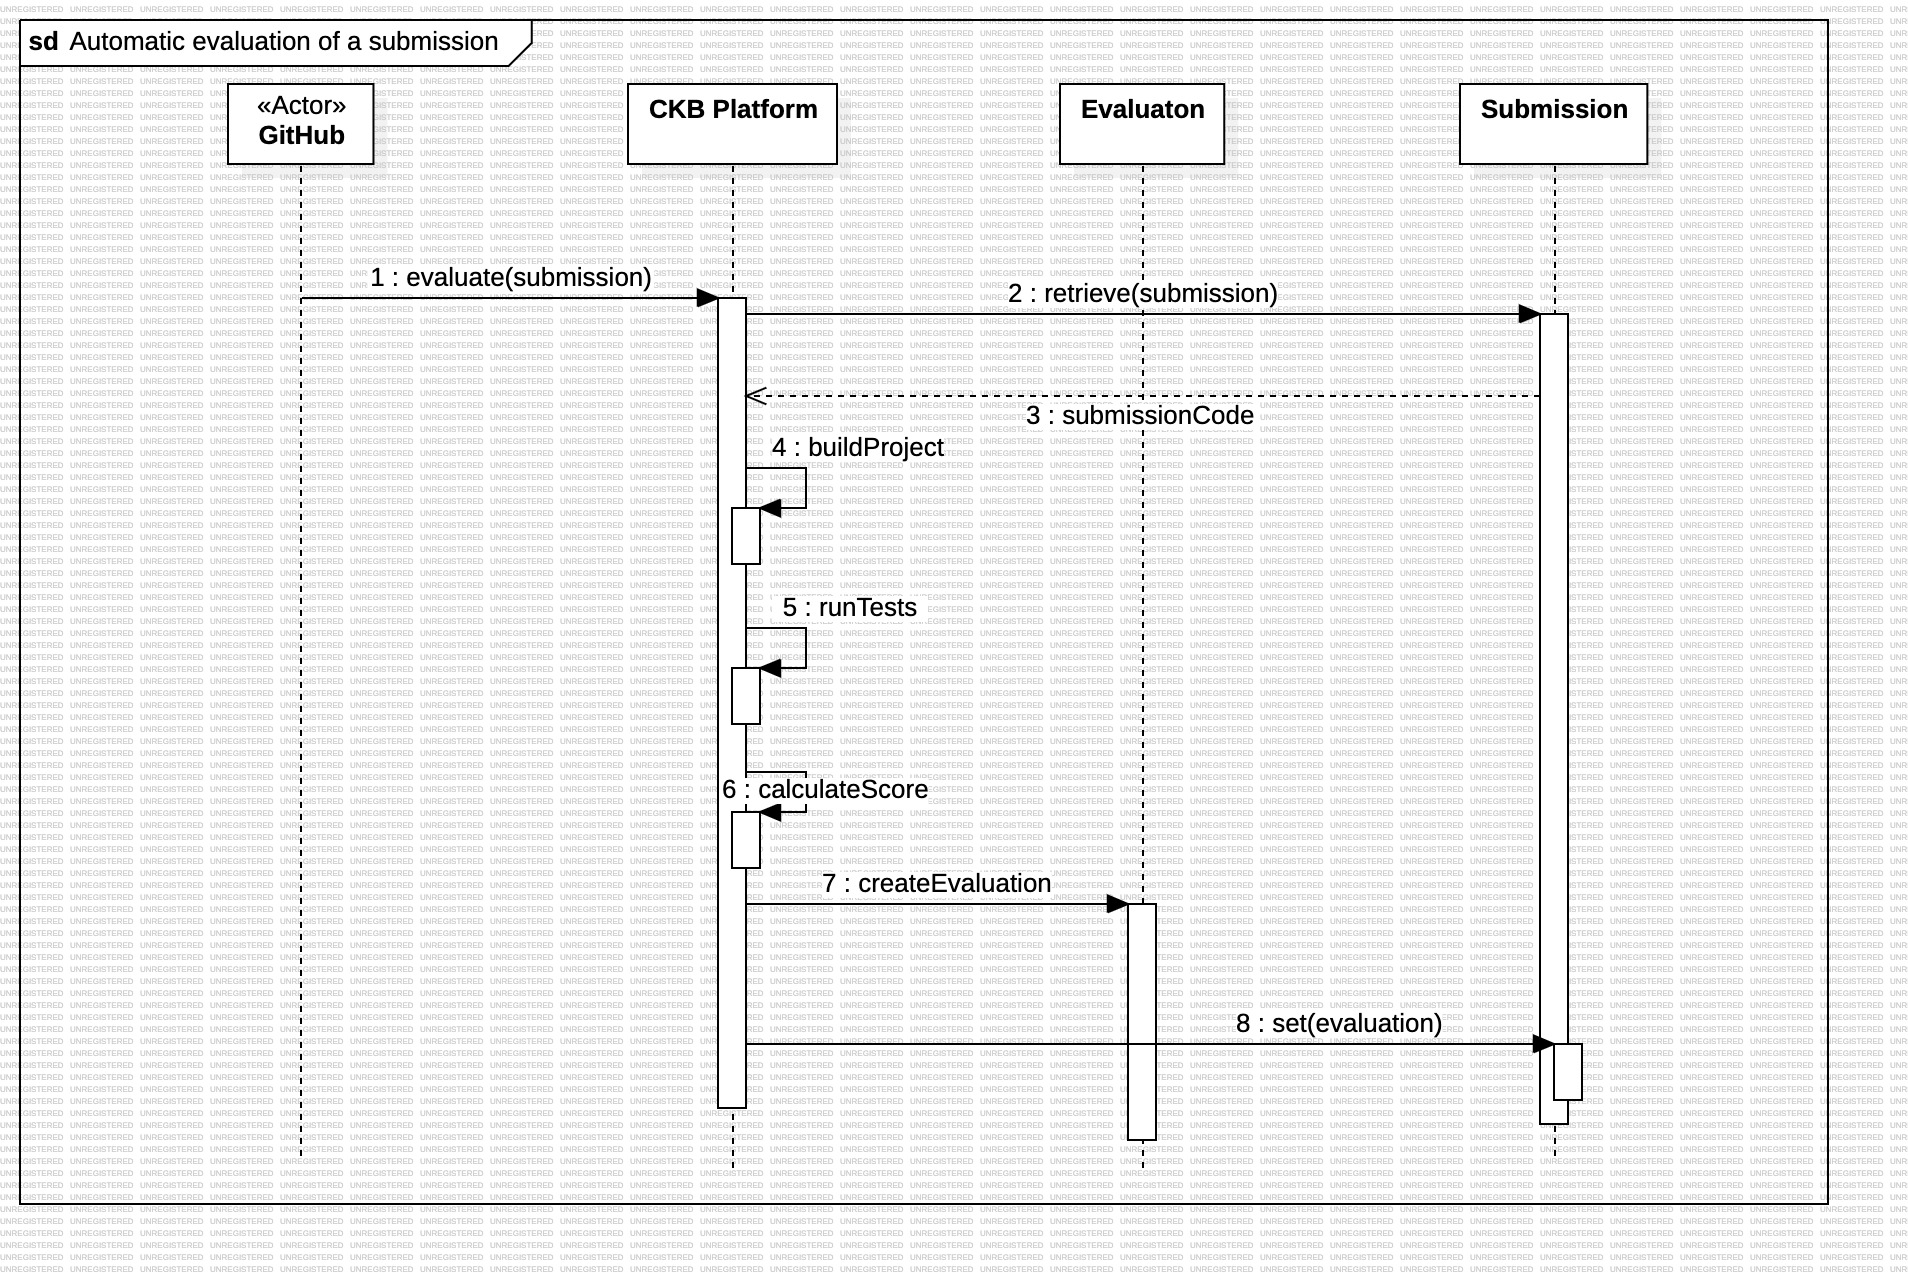
\includegraphics[width=\textwidth]{Diagrams/AutomaticEvaluation.jpg}
    \caption{Sequence Diagram - Automatic evaluation of a submission}
    \label{fig:sequence-diagram-automatic-evaluation}
\end{figure}

\subsubsection{Requirements mapping}
\begin{tabular}{|p{6cm}|p{6cm}|}
    \hline
    \multicolumn{2}{|c|}{[G1] Educator can create a torunament} \\
    \hline
    \begin{itemize}
        \item [R1]
        \item [R2]
        \item [R3]
    \end{itemize}
    &
    \begin{itemize}
        \item [D1]
        \item [D3]
    \end{itemize}
    \\
    \hline
\end{tabular}

\begin{tabular}{|p{6cm}|p{6cm}|}
    \hline
    \multicolumn{2}{|c|}{[G2] Educator can setup battles for a tournament} \\
    \hline
    \begin{itemize}
        \item [R1]
        \item [R2]
        \item [R4]
        \item [R5]
        \item [R6]
    \end{itemize}
    &
    \begin{itemize}
        \item [D1]
        \item [D3]
    \end{itemize}
    \\
    \hline
\end{tabular}

\begin{tabular}{|p{6cm}|p{6cm}|}
    \hline
    \multicolumn{2}{|c|}{[G3] Student can partecipate in a tournament} \\
    \hline
    \begin{itemize}
        \item [R1]
        \item [R2]
        \item [R7]
        \item [R8]
    \end{itemize}
    &
    \begin{itemize}
        \item [D1]
        \item [D2]
        \item [D3]
    \end{itemize}
    \\
    \hline
\end{tabular}

\begin{tabular}{|p{6cm}|p{6cm}|}
    \hline
    \multicolumn{2}{|c|}{[G4] Team of students can submit a solution for a battle} \\
    \hline
    \begin{itemize}
        \item [R1]
        \item [R2]
        \item [R7]
        \item [R8]
        \item [R9]
    \end{itemize}
    &
    \begin{itemize}
        \item [D1]
        \item [D2]
        \item [D3]
        \item [D4]
        \item [D8å]
    \end{itemize}
    \\
    \hline
\end{tabular}

\begin{tabular}{|p{6cm}|p{6cm}|}
    \hline
    \multicolumn{2}{|c|}{[G5] Educator can manually update the score of a team in a battle} \\
    \hline
    \begin{itemize}
        \item [R1]
        \item [R2]
        \item [R19]
    \end{itemize}
    &
    \begin{itemize}
        \item [D1]
        \item [D3]
        \item [D4]
        \item [D8]
        \item [D9]
    \end{itemize}
    \\
    \hline
\end{tabular}

\begin{tabular}{|p{6cm}|p{6cm}|}
    \hline
    \multicolumn{2}{|c|}{[G6] CKB notify the student about upcoming tournaments} \\
    \hline
    \begin{itemize}
        \item [R1]
        \item [R12]
    \end{itemize}
    &
    \begin{itemize}
        \item [D1]
        \item [D3]
        \item [D6]
    \end{itemize}
    \\
    \hline
\end{tabular}

\begin{tabular}{|p{6cm}|p{6cm}|}
    \hline
    \multicolumn{2}{|c|}{[G7] CKB notify the student about upcoming battles} \\
    \hline
    \begin{itemize}
        \item [R1]
        \item [R13]
    \end{itemize}
    &
    \begin{itemize}
        \item [D1]
        \item [D3]
        \item [D7]
    \end{itemize}
    \\
    \hline
\end{tabular}


%------------------------------------------------------------------------------------------------------------------------------------------------
\clearpage
{\color{Blue}{\section{Formal Analysis Using Alloy}}}
\label{sect:alloy}
Organize this section according to the rules defined in the project description. 


%------------------------------------------------------------------------------------------------------------------------------------------------
\clearpage
{\color{Blue}{\section{Effort Spent}}}
\label{sect:effort}
This section provides an estimation of the effort spent by each member of the group to redact this document. The time for each section includes the time spent to write, to discuss and to review the document itself.\\


\subsection*{Picone Paolo}
\begin{tabular}{|p{7cm}|p{7cm}|}
    \hline
    \textbf{Section} & \textbf{Hours}\\
    \hline
    1 & 6\\
    \hline
    2 & 13\\
    \hline
    3 & 23\\
    \hline
    4 & 8\\
    \hline
\end{tabular}


\subsection*{Russo Mario}
\begin{tabular}{|p{7cm}|p{7cm}|}
    \hline
    \textbf{Section} & \textbf{Hours}\\
    \hline
    1 & 6\\
    \hline
    2 & 14\\
    \hline
    3 & 22\\
    \hline
    4 & 8\\
    \hline
\end{tabular}



%------------------------------------------------------------------------------------------------------------------------------------------------
\clearpage
\addcontentsline{toc}{section}{References}
\bibliographystyle{plain}
\bibliography{main}
\begin{itemize}
        \item Document written using \LaTeX  \ and Visual Studio Code
        \item Diagrams created using StarUML 6.0.1
        \item Alloy code created using Alloy Analyzer 6.1.0
        \item Mockups created using Figma
\end{itemize}
%------------------------------------------------------------------------------------------------------------------------------------------------




\end{document}
